% Options for packages loaded elsewhere
\PassOptionsToPackage{unicode}{hyperref}
\PassOptionsToPackage{hyphens}{url}
\PassOptionsToPackage{dvipsnames,svgnames,x11names}{xcolor}
%
\documentclass[
  a4paper,
  DIV=11]{scrreprt}

\usepackage{amsmath,amssymb}
\usepackage{iftex}
\ifPDFTeX
  \usepackage[T1]{fontenc}
  \usepackage[utf8]{inputenc}
  \usepackage{textcomp} % provide euro and other symbols
\else % if luatex or xetex
  \usepackage{unicode-math}
  \defaultfontfeatures{Scale=MatchLowercase}
  \defaultfontfeatures[\rmfamily]{Ligatures=TeX,Scale=1}
\fi
\usepackage{lmodern}
\ifPDFTeX\else  
    % xetex/luatex font selection
    \setmainfont[]{Times New Roman}
    \setsansfont[]{Arial}
    \setmonofont[]{Courier New}
\fi
% Use upquote if available, for straight quotes in verbatim environments
\IfFileExists{upquote.sty}{\usepackage{upquote}}{}
\IfFileExists{microtype.sty}{% use microtype if available
  \usepackage[]{microtype}
  \UseMicrotypeSet[protrusion]{basicmath} % disable protrusion for tt fonts
}{}
\makeatletter
\@ifundefined{KOMAClassName}{% if non-KOMA class
  \IfFileExists{parskip.sty}{%
    \usepackage{parskip}
  }{% else
    \setlength{\parindent}{0pt}
    \setlength{\parskip}{6pt plus 2pt minus 1pt}}
}{% if KOMA class
  \KOMAoptions{parskip=half}}
\makeatother
\usepackage{xcolor}
\ifLuaTeX
  \usepackage{luacolor}
  \usepackage[soul]{lua-ul}
\else
  \usepackage{soul}
  
\fi
\setlength{\emergencystretch}{3em} % prevent overfull lines
\setcounter{secnumdepth}{5}
% Make \paragraph and \subparagraph free-standing
\makeatletter
\ifx\paragraph\undefined\else
  \let\oldparagraph\paragraph
  \renewcommand{\paragraph}{
    \@ifstar
      \xxxParagraphStar
      \xxxParagraphNoStar
  }
  \newcommand{\xxxParagraphStar}[1]{\oldparagraph*{#1}\mbox{}}
  \newcommand{\xxxParagraphNoStar}[1]{\oldparagraph{#1}\mbox{}}
\fi
\ifx\subparagraph\undefined\else
  \let\oldsubparagraph\subparagraph
  \renewcommand{\subparagraph}{
    \@ifstar
      \xxxSubParagraphStar
      \xxxSubParagraphNoStar
  }
  \newcommand{\xxxSubParagraphStar}[1]{\oldsubparagraph*{#1}\mbox{}}
  \newcommand{\xxxSubParagraphNoStar}[1]{\oldsubparagraph{#1}\mbox{}}
\fi
\makeatother

\usepackage{color}
\usepackage{fancyvrb}
\newcommand{\VerbBar}{|}
\newcommand{\VERB}{\Verb[commandchars=\\\{\}]}
\DefineVerbatimEnvironment{Highlighting}{Verbatim}{commandchars=\\\{\}}
% Add ',fontsize=\small' for more characters per line
\usepackage{framed}
\definecolor{shadecolor}{RGB}{241,243,245}
\newenvironment{Shaded}{\begin{snugshade}}{\end{snugshade}}
\newcommand{\AlertTok}[1]{\textcolor[rgb]{0.68,0.00,0.00}{#1}}
\newcommand{\AnnotationTok}[1]{\textcolor[rgb]{0.37,0.37,0.37}{#1}}
\newcommand{\AttributeTok}[1]{\textcolor[rgb]{0.40,0.45,0.13}{#1}}
\newcommand{\BaseNTok}[1]{\textcolor[rgb]{0.68,0.00,0.00}{#1}}
\newcommand{\BuiltInTok}[1]{\textcolor[rgb]{0.00,0.23,0.31}{#1}}
\newcommand{\CharTok}[1]{\textcolor[rgb]{0.13,0.47,0.30}{#1}}
\newcommand{\CommentTok}[1]{\textcolor[rgb]{0.37,0.37,0.37}{#1}}
\newcommand{\CommentVarTok}[1]{\textcolor[rgb]{0.37,0.37,0.37}{\textit{#1}}}
\newcommand{\ConstantTok}[1]{\textcolor[rgb]{0.56,0.35,0.01}{#1}}
\newcommand{\ControlFlowTok}[1]{\textcolor[rgb]{0.00,0.23,0.31}{\textbf{#1}}}
\newcommand{\DataTypeTok}[1]{\textcolor[rgb]{0.68,0.00,0.00}{#1}}
\newcommand{\DecValTok}[1]{\textcolor[rgb]{0.68,0.00,0.00}{#1}}
\newcommand{\DocumentationTok}[1]{\textcolor[rgb]{0.37,0.37,0.37}{\textit{#1}}}
\newcommand{\ErrorTok}[1]{\textcolor[rgb]{0.68,0.00,0.00}{#1}}
\newcommand{\ExtensionTok}[1]{\textcolor[rgb]{0.00,0.23,0.31}{#1}}
\newcommand{\FloatTok}[1]{\textcolor[rgb]{0.68,0.00,0.00}{#1}}
\newcommand{\FunctionTok}[1]{\textcolor[rgb]{0.28,0.35,0.67}{#1}}
\newcommand{\ImportTok}[1]{\textcolor[rgb]{0.00,0.46,0.62}{#1}}
\newcommand{\InformationTok}[1]{\textcolor[rgb]{0.37,0.37,0.37}{#1}}
\newcommand{\KeywordTok}[1]{\textcolor[rgb]{0.00,0.23,0.31}{\textbf{#1}}}
\newcommand{\NormalTok}[1]{\textcolor[rgb]{0.00,0.23,0.31}{#1}}
\newcommand{\OperatorTok}[1]{\textcolor[rgb]{0.37,0.37,0.37}{#1}}
\newcommand{\OtherTok}[1]{\textcolor[rgb]{0.00,0.23,0.31}{#1}}
\newcommand{\PreprocessorTok}[1]{\textcolor[rgb]{0.68,0.00,0.00}{#1}}
\newcommand{\RegionMarkerTok}[1]{\textcolor[rgb]{0.00,0.23,0.31}{#1}}
\newcommand{\SpecialCharTok}[1]{\textcolor[rgb]{0.37,0.37,0.37}{#1}}
\newcommand{\SpecialStringTok}[1]{\textcolor[rgb]{0.13,0.47,0.30}{#1}}
\newcommand{\StringTok}[1]{\textcolor[rgb]{0.13,0.47,0.30}{#1}}
\newcommand{\VariableTok}[1]{\textcolor[rgb]{0.07,0.07,0.07}{#1}}
\newcommand{\VerbatimStringTok}[1]{\textcolor[rgb]{0.13,0.47,0.30}{#1}}
\newcommand{\WarningTok}[1]{\textcolor[rgb]{0.37,0.37,0.37}{\textit{#1}}}

\providecommand{\tightlist}{%
  \setlength{\itemsep}{0pt}\setlength{\parskip}{0pt}}\usepackage{longtable,booktabs,array}
\usepackage{calc} % for calculating minipage widths
% Correct order of tables after \paragraph or \subparagraph
\usepackage{etoolbox}
\makeatletter
\patchcmd\longtable{\par}{\if@noskipsec\mbox{}\fi\par}{}{}
\makeatother
% Allow footnotes in longtable head/foot
\IfFileExists{footnotehyper.sty}{\usepackage{footnotehyper}}{\usepackage{footnote}}
\makesavenoteenv{longtable}
\usepackage{graphicx}
\makeatletter
\def\maxwidth{\ifdim\Gin@nat@width>\linewidth\linewidth\else\Gin@nat@width\fi}
\def\maxheight{\ifdim\Gin@nat@height>\textheight\textheight\else\Gin@nat@height\fi}
\makeatother
% Scale images if necessary, so that they will not overflow the page
% margins by default, and it is still possible to overwrite the defaults
% using explicit options in \includegraphics[width, height, ...]{}
\setkeys{Gin}{width=\maxwidth,height=\maxheight,keepaspectratio}
% Set default figure placement to htbp
\makeatletter
\def\fps@figure{htbp}
\makeatother
% definitions for citeproc citations
\NewDocumentCommand\citeproctext{}{}
\NewDocumentCommand\citeproc{mm}{%
  \begingroup\def\citeproctext{#2}\cite{#1}\endgroup}
\makeatletter
 % allow citations to break across lines
 \let\@cite@ofmt\@firstofone
 % avoid brackets around text for \cite:
 \def\@biblabel#1{}
 \def\@cite#1#2{{#1\if@tempswa , #2\fi}}
\makeatother
\newlength{\cslhangindent}
\setlength{\cslhangindent}{1.5em}
\newlength{\csllabelwidth}
\setlength{\csllabelwidth}{3em}
\newenvironment{CSLReferences}[2] % #1 hanging-indent, #2 entry-spacing
 {\begin{list}{}{%
  \setlength{\itemindent}{0pt}
  \setlength{\leftmargin}{0pt}
  \setlength{\parsep}{0pt}
  % turn on hanging indent if param 1 is 1
  \ifodd #1
   \setlength{\leftmargin}{\cslhangindent}
   \setlength{\itemindent}{-1\cslhangindent}
  \fi
  % set entry spacing
  \setlength{\itemsep}{#2\baselineskip}}}
 {\end{list}}
\usepackage{calc}
\newcommand{\CSLBlock}[1]{\hfill\break\parbox[t]{\linewidth}{\strut\ignorespaces#1\strut}}
\newcommand{\CSLLeftMargin}[1]{\parbox[t]{\csllabelwidth}{\strut#1\strut}}
\newcommand{\CSLRightInline}[1]{\parbox[t]{\linewidth - \csllabelwidth}{\strut#1\strut}}
\newcommand{\CSLIndent}[1]{\hspace{\cslhangindent}#1}

% load packages
%\usepackage{multicol}
\usepackage{fontspec}
\usepackage{emoji}
\usepackage{xltxtra}
%\usepackage{xcolor}
\usepackage{listings}
\usepackage{fvextra}


\definecolor{ycol}{RGB}{230,159,0}
\definecolor{modelcol}{RGB}{86,180,233}
\definecolor{errorcol}{RGB}{0,158,115}
\definecolor{beta0col}{RGB}{213,94,0}
\definecolor{beta1col}{RGB}{0,114,178}
\definecolor{xcol}{RGB}{204,121,167}


\lstset{
  breaklines=true
}

\DefineVerbatimEnvironment{Highlighting}{Verbatim}{breaklines,commandchars=\\\{\}}
\DefineVerbatimEnvironment{OutputCode}{Verbatim}{breaklines,commandchars=\\\{\}}
\KOMAoption{captions}{tableheading}
\makeatletter
\@ifpackageloaded{tcolorbox}{}{\usepackage[skins,breakable]{tcolorbox}}
\@ifpackageloaded{fontawesome5}{}{\usepackage{fontawesome5}}
\definecolor{quarto-callout-color}{HTML}{909090}
\definecolor{quarto-callout-note-color}{HTML}{0758E5}
\definecolor{quarto-callout-important-color}{HTML}{CC1914}
\definecolor{quarto-callout-warning-color}{HTML}{EB9113}
\definecolor{quarto-callout-tip-color}{HTML}{00A047}
\definecolor{quarto-callout-caution-color}{HTML}{FC5300}
\definecolor{quarto-callout-color-frame}{HTML}{acacac}
\definecolor{quarto-callout-note-color-frame}{HTML}{4582ec}
\definecolor{quarto-callout-important-color-frame}{HTML}{d9534f}
\definecolor{quarto-callout-warning-color-frame}{HTML}{f0ad4e}
\definecolor{quarto-callout-tip-color-frame}{HTML}{02b875}
\definecolor{quarto-callout-caution-color-frame}{HTML}{fd7e14}
\makeatother
\makeatletter
\@ifpackageloaded{caption}{}{\usepackage{caption}}
\AtBeginDocument{%
\ifdefined\contentsname
  \renewcommand*\contentsname{Inhaltsverzeichnis}
\else
  \newcommand\contentsname{Inhaltsverzeichnis}
\fi
\ifdefined\listfigurename
  \renewcommand*\listfigurename{Abbildungsverzeichnis}
\else
  \newcommand\listfigurename{Abbildungsverzeichnis}
\fi
\ifdefined\listtablename
  \renewcommand*\listtablename{Tabellenverzeichnis}
\else
  \newcommand\listtablename{Tabellenverzeichnis}
\fi
\ifdefined\figurename
  \renewcommand*\figurename{Abbildung}
\else
  \newcommand\figurename{Abbildung}
\fi
\ifdefined\tablename
  \renewcommand*\tablename{Tabelle}
\else
  \newcommand\tablename{Tabelle}
\fi
}
\@ifpackageloaded{float}{}{\usepackage{float}}
\floatstyle{ruled}
\@ifundefined{c@chapter}{\newfloat{codelisting}{h}{lop}}{\newfloat{codelisting}{h}{lop}[chapter]}
\floatname{codelisting}{Listing}
\newcommand*\listoflistings{\listof{codelisting}{Listingverzeichnis}}
\usepackage{amsthm}
\theoremstyle{definition}
\newtheorem{example}{Beispiel}[chapter]
\theoremstyle{definition}
\newtheorem{definition}{Definition}[chapter]
\theoremstyle{remark}
\AtBeginDocument{\renewcommand*{\proofname}{Beweis}}
\newtheorem*{remark}{Anmerkung}
\newtheorem*{solution}{Lösung}
\newtheorem{refremark}{Anmerkung}[chapter]
\newtheorem{refsolution}{Lösung}[chapter]
\makeatother
\makeatletter
\makeatother
\makeatletter
\@ifpackageloaded{caption}{}{\usepackage{caption}}
\@ifpackageloaded{subcaption}{}{\usepackage{subcaption}}
\makeatother

\ifLuaTeX
\usepackage[bidi=basic]{babel}
\else
\usepackage[bidi=default]{babel}
\fi
\babelprovide[main,import]{ngerman}
\ifPDFTeX
\else
\babelfont{rm}[]{Times New Roman}
\fi
% get rid of language-specific shorthands (see #6817):
\let\LanguageShortHands\languageshorthands
\def\languageshorthands#1{}
\ifLuaTeX
  \usepackage{selnolig}  % disable illegal ligatures
\fi
\usepackage{bookmark}

\IfFileExists{xurl.sty}{\usepackage{xurl}}{} % add URL line breaks if available
\urlstyle{same} % disable monospaced font for URLs
\hypersetup{
  pdftitle={Statistik1},
  pdfauthor={Sebastian Sauer},
  pdflang={de},
  colorlinks=true,
  linkcolor={blue},
  filecolor={Maroon},
  citecolor={Blue},
  urlcolor={Blue},
  pdfcreator={LaTeX via pandoc}}


\title{Statistik1}
\author{Sebastian Sauer}
\date{2024-08-29}

\begin{document}
\maketitle

\renewcommand*\contentsname{Inhaltsverzeichnis}
{
\hypersetup{linkcolor=}
\setcounter{tocdepth}{2}
\tableofcontents
}

\chapter{Willkommen!}\label{willkommen}

\begin{figure}[H]

{\centering 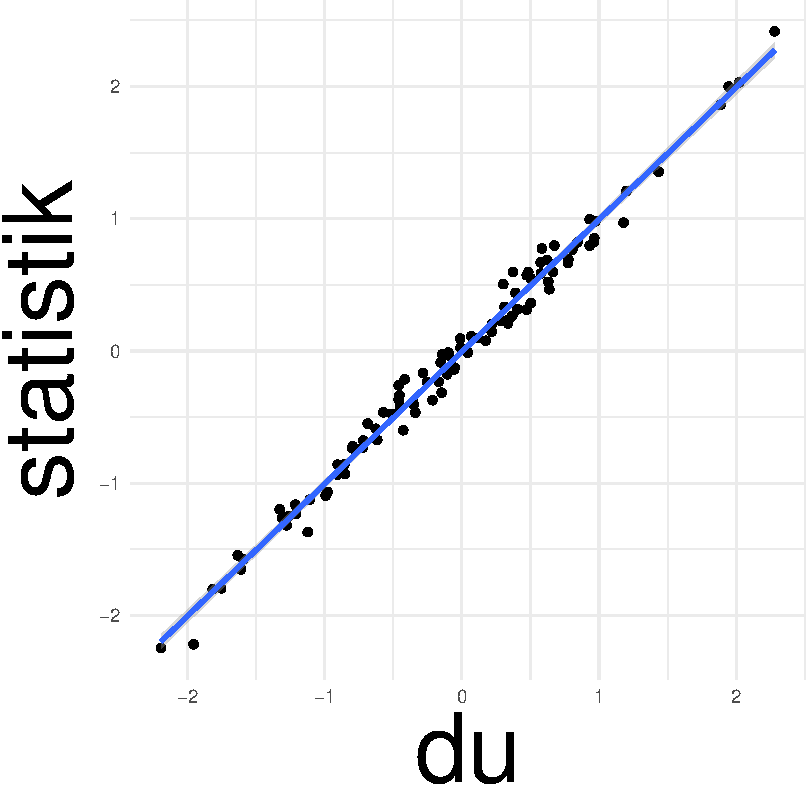
\includegraphics[width=0.33\textwidth,height=\textheight]{index_files/figure-pdf/unnamed-chunk-1-1.pdf}

}

\caption{Statistik und Du: Guter Fit!}

\end{figure}%

\section{Es geht um Ihren Lernerfolg}\label{es-geht-um-ihren-lernerfolg}

Meister Yoda rät: Lesen Sie die Hinweise (Abbildung~\ref{fig-yoda}).

\begin{figure}

\centering{


\includegraphics[width=0.5\textwidth,height=\textheight]{img/yoda.jpg}

}

\caption{\label{fig-yoda}Lesen Sie die folgenden Hinweise im eigenen
Interesse}

\end{figure}%

\href{https://imgflip.com/memegenerator}{Quelle: Imgflip Memengenerator}

\subsection{Lernziele}\label{lernziele}

\begin{itemize}
\item
  Die Studentis sind mit wesentlichen Methoden der explorativen
  Datenanalyse vertraut und können diese selbständig anwenden.
\item
  Die Studentis können gängige Forschungsfragen in lineare Modelle
  übersetzen, diese auf echte Datensätze anwenden und die Ergebnisse
  interpretieren.
\end{itemize}

Kurz gesagt: Das ist ein Grundkurs in Daten zähmen.

\begin{figure}[H]

{\centering 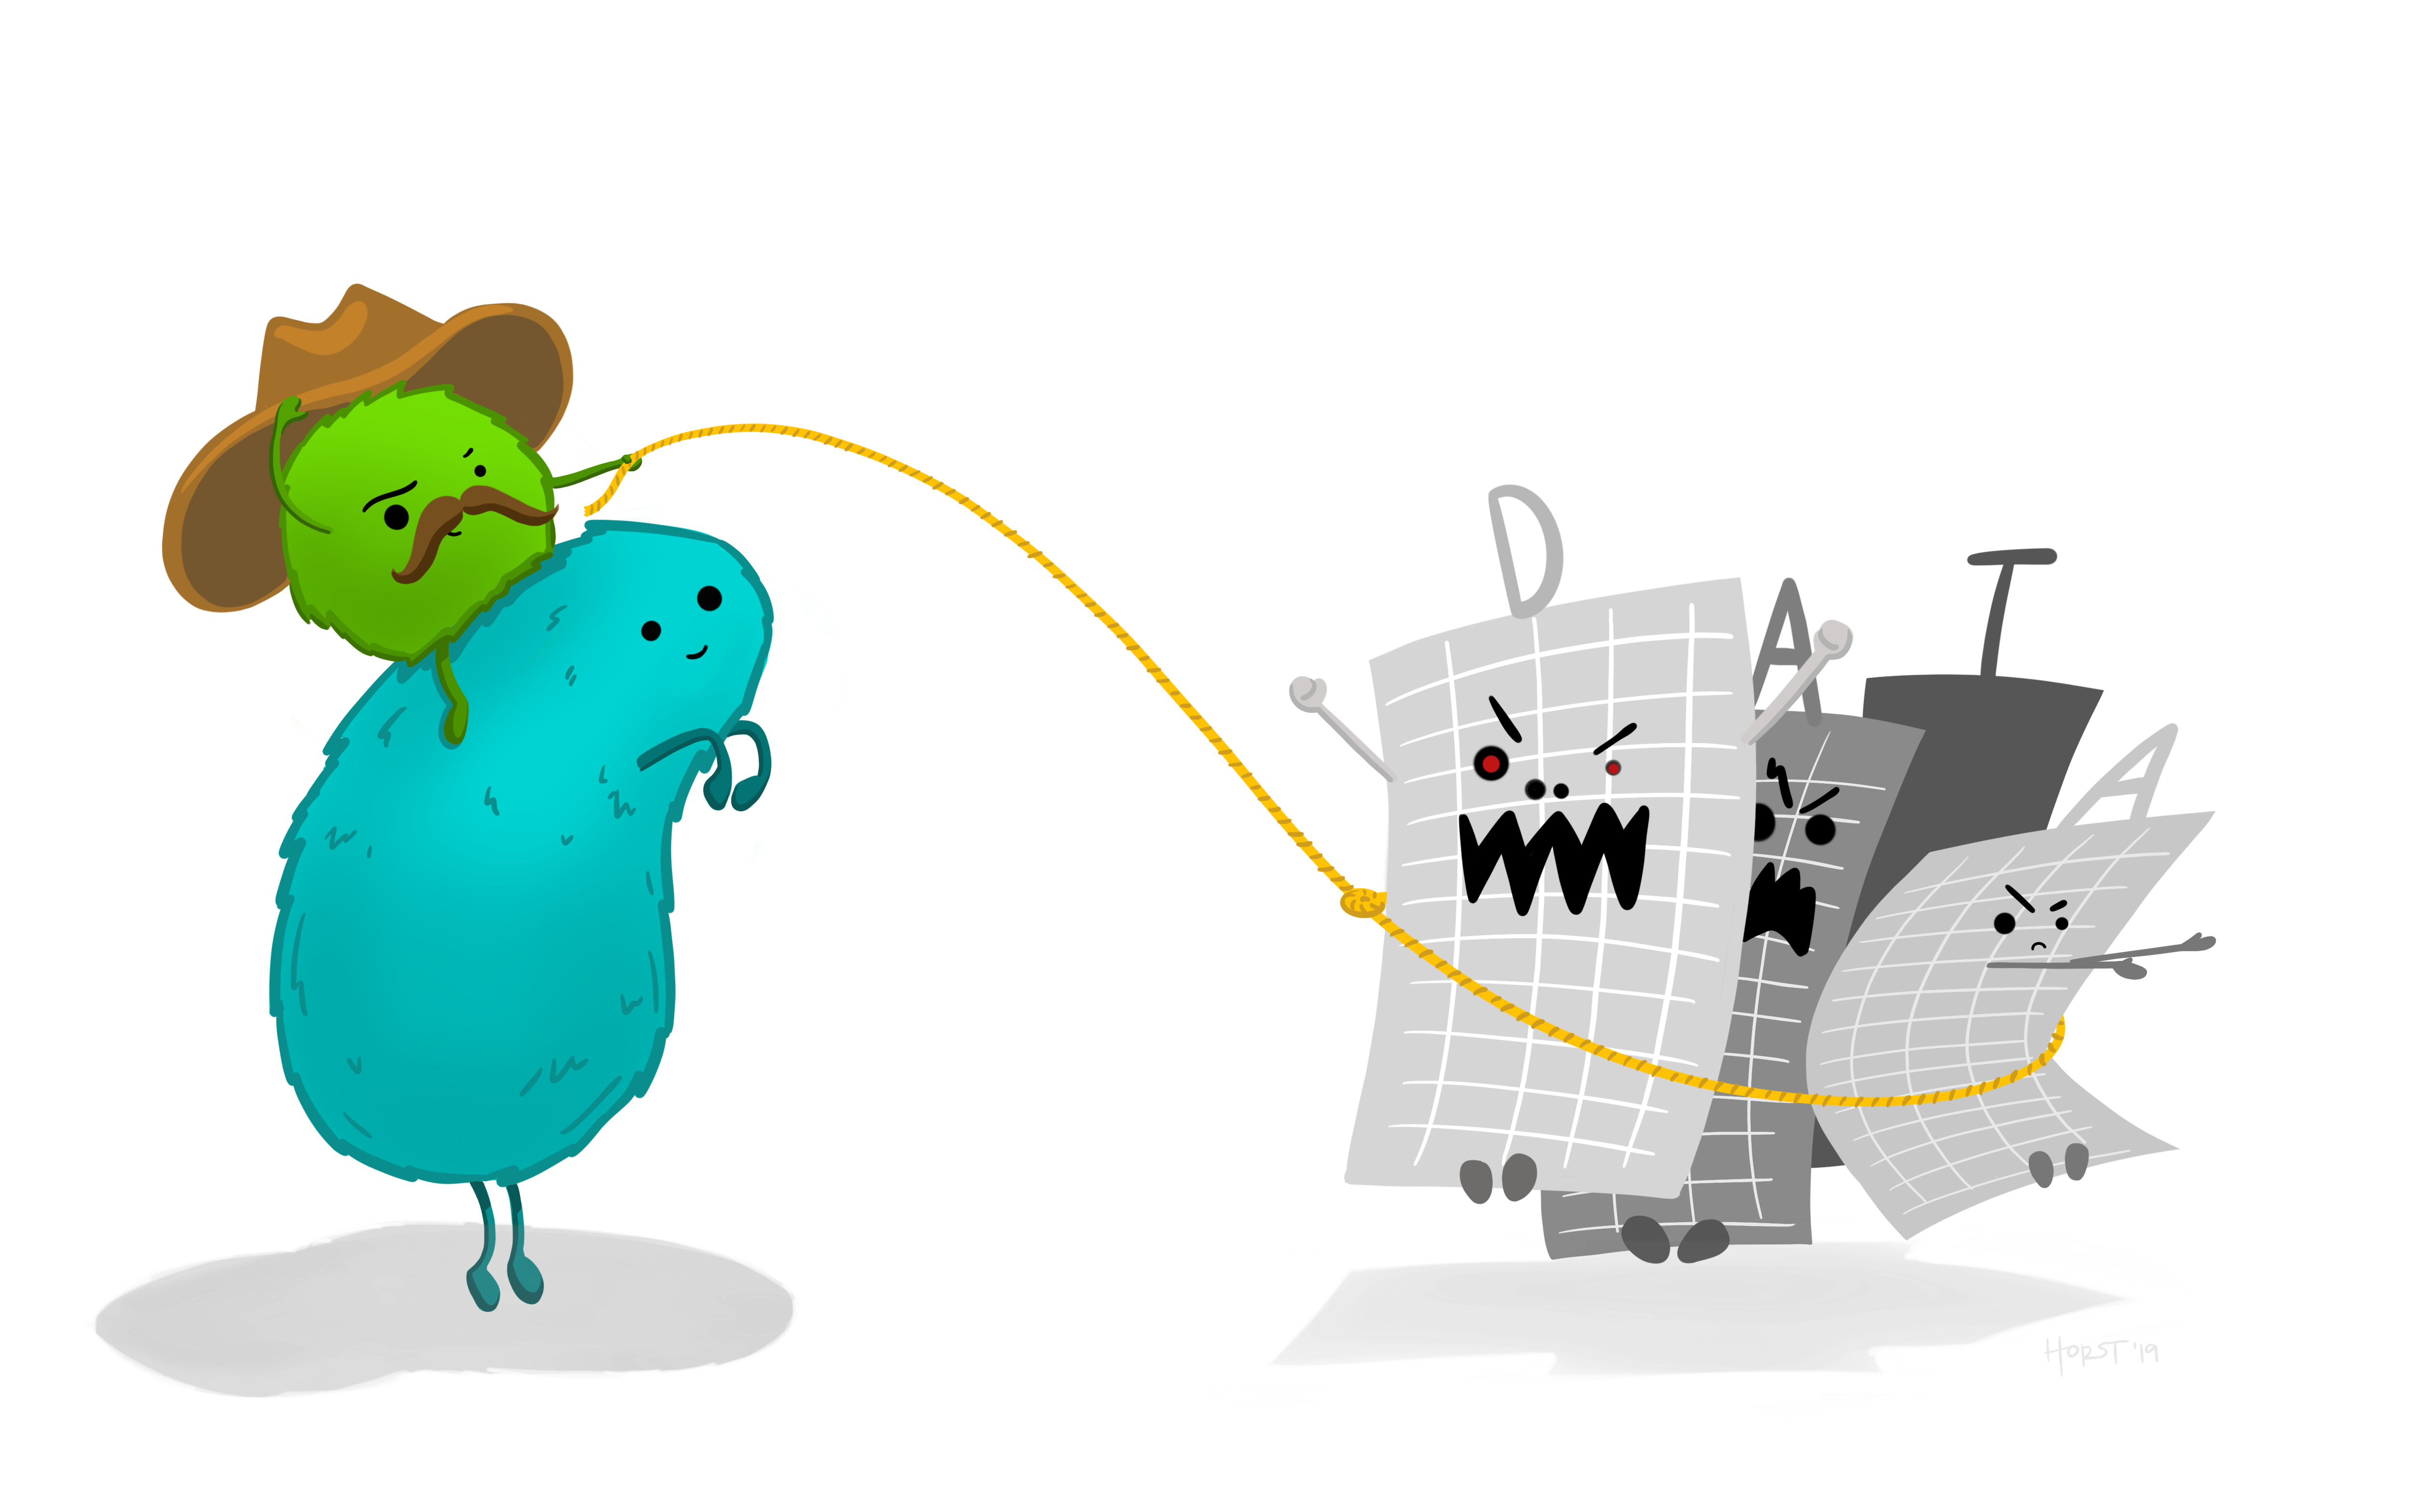
\includegraphics[width=0.5\textwidth,height=\textheight]{img/datenzaehmen.png}

}

\caption{Daten zähmen}

\end{figure}%

\href{https://github.com/allisonhorst/stats-illustrations}{Bildquelle:
Allison Horst, CC-BY}

\subsection{Was lerne ich hier und wozu ist das
gut?}\label{was-lerne-ich-hier-und-wozu-ist-das-gut}

\emph{Was lerne ich hier?}

Sie lernen das \emph{Handwerk der Datenanalyse} mit einem Schwerpunkt
auf Vorhersage. Anders gesagt: Sie lernen, \emph{Daten aufzubereiten}
und aus Daten \emph{Vorhersagen} abzuleiten. Zum Beispiel: Kommt ein
Student zu Ihnen und sagt ``Ich habe 42 Stunden für die Klausur gelernt,
welche Note kann ich in der Klausur erwarten?''. Darauf Ihre Antwort:
``Auf Basis meiner Daten und meines Modells müsstest du eine 2.7
schreiben!''.\footnote{Darauf dis Studenti: ``Hpmf.''}. Außerdem lernen
Sie, wie man die Güte einer Vorhersage auf Stichhaltigkeit prüft. Denn
Vorhersagen kann man ja in jeder Eckkneipe oder beim Wahrsager bekommen.
Wir wollen aber belastbare Vorhersagen und zumindest wissen, wie gut die
Vorhersagen (von jemanden) bisher waren.

\emph{Warum ist das wichtig?}

Wir wollen nicht auf Leuten vertrauen, die behaupten, sie wüssten, was
für uns richtig und gut ist. Wir wollen selber die Fakten prüfen können.

\emph{Wozu brauche ich das im Job?}

Datenanalyse spielt bereits heute in vielen Berufen eine Rolle. Tendenz
stark zunehmend.

\emph{Wozu brauche ich das im weiterem Studium?}

In Forschungsarbeiten (wie in empirischen Forschungsprojekten, etwa in
der Abschlussarbeit) ist es üblich, statistische Ergebnisse hinsichtlich
quantitativ zu analysieren.

\emph{Ist Statistik nicht sehr abstrakt?}

Der Schwerpunkt dieses Kurses liegt auf Anwenden und Tun; ähnlich dem
Erlernen eines Handwerks. Theorien und Abstraktionen stehen nur am Rand.

\emph{Gibt es auch gute Jobs, wenn man sich mit Daten auskennt?}

Das Forum (2020) berichtet zu den ``Top 20 job roles in increasing and
decreasing demand across industries'' (S. 30, Abb. 22):

\begin{enumerate}
\def\labelenumi{\arabic{enumi}.}
\tightlist
\item
  Data Analysts und Scientists
\item
  AI and Machine Learning Specialists
\item
  Big Data Specialists
\end{enumerate}

\subsection{Was ist hier das
Erfolgsgeheimnis?}\label{was-ist-hier-das-erfolgsgeheimnis}

\begin{tcolorbox}[enhanced jigsaw, bottomtitle=1mm, title=\textcolor{quarto-callout-important-color}{\faExclamation}\hspace{0.5em}{Wichtig}, toptitle=1mm, arc=.35mm, bottomrule=.15mm, breakable, colbacktitle=quarto-callout-important-color!10!white, left=2mm, colframe=quarto-callout-important-color-frame, colback=white, opacityback=0, titlerule=0mm, rightrule=.15mm, opacitybacktitle=0.6, leftrule=.75mm, toprule=.15mm, coltitle=black]

\emph{Dran bleiben} ist der Schlüssel zum Erfolg. Üben Sie regelmäßig.
Geben Sie bei Schwierigkeiten nicht auf.

\emoji{person-lifting-weights} \emoji{clockwise-vertical-arrows}
\emoji{key} \emoji{glowing-star} \(\square\)

\end{tcolorbox}

\subsection{Motivieren Sie mich!}\label{motivieren-sie-mich}

Schauen Sie sich das Video mit einer
\href{https://youtu.be/jtNlzpcPr5Y}{Ansprache zur Motivation}
an.\footnote{\url{https://youtu.be/jtNlzpcPr5Y}}

\subsection{Voraussetzungen}\label{voraussetzungen}

Um von diesem Kurs am besten zu profitieren, sollten Sie Folgendes
mitbringen:

\begin{itemize}
\tightlist
\item
  Bereitschaft, Neues zu lernen
\item
  Bereitschaft, nicht gleich aufzugeben
\item
  Kenntnis grundlegender Methoden wissenschaftlichen Arbeitens
\end{itemize}

Was Sie \emph{nicht} brauchen, sind besondere Mathe-Vorkenntnisse.

\subsection{Überblick}\label{uxfcberblick}

Abb. Abbildung~\ref{fig-ueberblick} gibt einen Überblick über den
Verlauf und die Inhalte des Buches. Das Diagramm hilft Ihnen zu
verorten, wo welches Thema im Gesamtzusammenhang steht.

\begin{figure}

\centering{

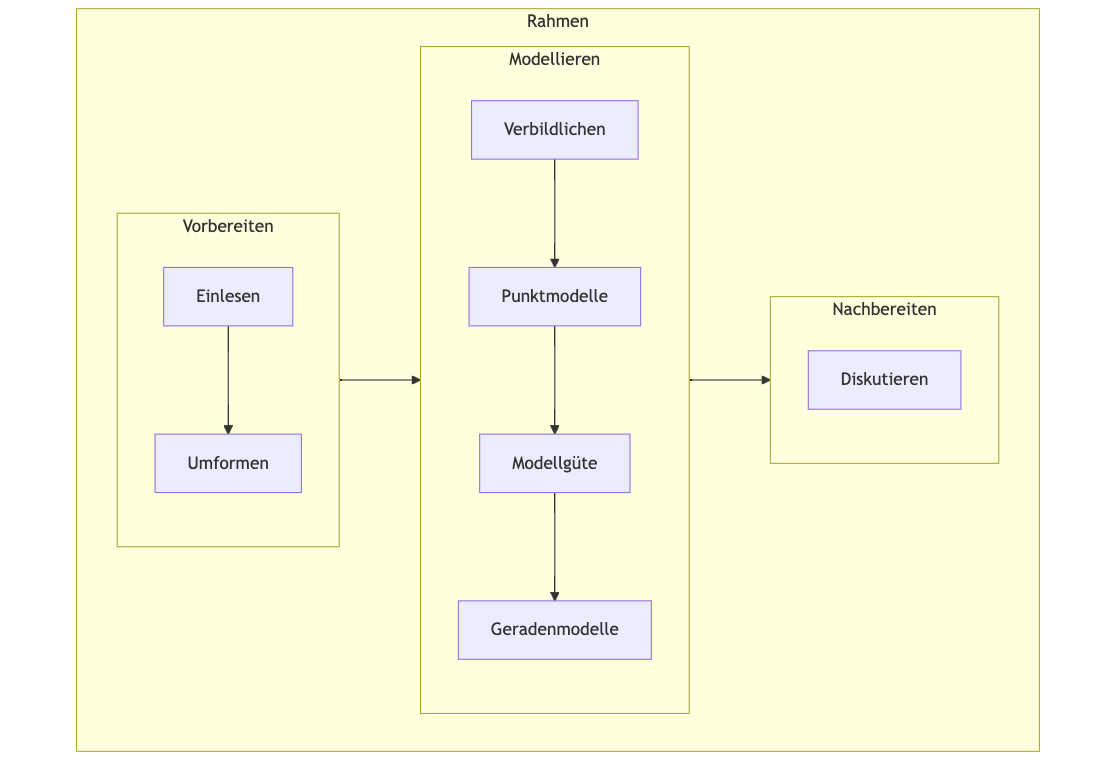
\includegraphics{img/fig-ueberblick.png}

}

\caption{\label{fig-ueberblick}Überblick über den Inhalt und Verlauf des
Buches}

\end{figure}%

Das Diagramm zeigt den Ablauf einer typischen Datenanalyse. Natürlich
kann man sich auch andere sinnvolle Darstellungen dieses Ablaufs
vorstellen.

\section{Software}\label{software}

Sie benötigen R, RStudio und einige R-Pakete für diesen Kurs.

\subsection{Installation}\label{installation}

\href{https://hinweisbuch.netlify.app/hinweise-software}{Hier} finden
Sie \emph{Installationshinweise.}\footnote{\url{https://hinweisbuch.netlify.app/hinweise-software}}

\subsection{Viel R (?)}\label{viel-r}

Dieses Buch enthält ``mittel'' viel R. Auf fortgeschrittene R-Techniken
wurde aber komplett verzichtet. Dem einen oder der anderen Anfänger:in
mag es dennoch ``viel Code'' erscheinen. Es wäre ja auch möglich
gewesen, auf R zu verzichten und stattdessen eine ``Klick-Software'' zu
verwenden. \href{https://jasp-stats.org/}{JASP} oder
\href{https://www.jamovi.org/}{Jamovi} sind Beispiele für tolle Software
aus dieser Kategorie. Ich glaube aber, der Verzicht auf eine
Skriptsprache (R) wäre ein schlechter Dienst an den Studentis. Mit Blick
auf eine ``High-Tech-Zukunft'' sollte man zumindest mit etwas
Computer-Code vertraut sein. Auf Computercode zu verzichten erschiene
mir daher fahrlässig für die ``Zukunftsfestigkeit'' der Ausbildung.

\section{Zum Autor}\label{zum-autor}

Nähere Hinweise zum Autor dieses Buch, Sebastian Sauer, finden Sie
\href{https://sebastiansauer-academic.netlify.app/}{hier}.\footnote{\url{https://sebastiansauer-academic.netlify.app/}}
Dort gibt es auch einen Überblick über
\href{https://sebastiansauer-academic.netlify.app/\#ebooks}{weitere
Bücher des Autors zum Themenkreis Datenanalyse}.\footnote{\url{https://sebastiansauer-academic.netlify.app/\#ebooks}}

\section{Nomenklatur}\label{nomenklatur}

\subsection{Griechische Buchstaben}\label{sec-greek}

In diesem Buch werden ein paar (wenige) griechische Buchstaben
verwendet, die in der Statistik üblich sind. Häufig werden
\emph{griechische} Buchstaben verwendet, um eine Grundgesamtheit
(Population) zu beschreiben (die meistens unbekannt ist). Lateinische
(``normale'') Buchstaben werden demgegenüber verwendet, um eine
Stichprobe (Datensatz, vorliegende Daten) zu beschreiben.
Tabelle~\ref{tbl-griech} stellt diese Buchstaben zusammen mit ihrer
Aussprache und Bedeutung vor.

\begin{longtable}[]{@{}lllr@{}}
\caption{Griechische Buchstaben, die in diesem Buch verwendet
werden.}\label{tbl-griech}\tabularnewline
\toprule\noalign{}
Zeichen & Aussprache & Buchstabe & Bedeutung in der Statistik \\
\midrule\noalign{}
\endfirsthead
\toprule\noalign{}
Zeichen & Aussprache & Buchstabe & Bedeutung in der Statistik \\
\midrule\noalign{}
\endhead
\bottomrule\noalign{}
\endlastfoot
\(\beta\) & beta & b & Regressionskoeffizent \\
\(\mu\) & mü & m & Mittelwert \\
\(\sigma\) & sigma & s & Streuung \\
\(\Sigma\) & Sigma & S & Summenzeichen \\
\(\rho\) & rho & r & Korrelation (nach Pearson) \\
\end{longtable}

Mehr griechische Buchstaben finden sich
\href{https://de.wikipedia.org/wiki/Griechisches_Alphabet}{z.B. in
Wikipedia}.\footnote{\url{https://de.wikipedia.org/wiki/Griechisches_Alphabet}}

\section{Zitation}\label{zitation}

Bitte zitieren Sie dieses Buch wie folgt:

\begin{quote}
Sauer, S. (2024). \emph{Statistik1}. https://statistik1.netlify.app/
\end{quote}

Hier sind die maschinenlesbaren Zitationsinfos (Bibtex-Format), die Sie
in Ihre Literatursoftware importieren können:

\begin{verbatim}
@book{sauer_statistik1,
    title = {Statistik1},
    rights = {CC-BY-NC},
    url = {https://statistik1.netlify.app/},
    author = {Sauer, Sebastian},
    date = {2024},
}
\end{verbatim}

Hier ist die DOI:

\href{https://zenodo.org/doi/10.5281/zenodo.10082517}{10.5281/zenodo.10082517}

\section{Reproduzierbarkeit}\label{reproduzierbarkeit}

Die verwendeten R-Pakete sind mit
\href{https://rstudio.github.io/renv/index.html}{renv}
dokumentiert.\footnote{\url{https://rstudio.github.io/renv/index.html}}

Der Quellcode ist \href{https://github.com/sebastiansauer/statistik1}{in
diesem Github-Repo} dokumentiert.\footnote{\url{https://github.com/sebastiansauer/statistik1}}

Dieses Dokument wurde erzeugt am/um: 2024-08-29 09:33:27.

\part{Organisatorisches}

\part{Modellieren}

\chapter{Geradenmodelle 2}\label{geradenmodelle-2}

\section{Lernsteuerung}\label{lernsteuerung}

\subsection{Standort im Lernpfad}\label{standort-im-lernpfad}

Abb. Abbildung~\ref{fig-ueberblick} zeigt den Standort dieses Kapitels
im Lernpfad und gibt damit einen Überblick über das Thema dieses
Kapitels im Kontext aller Kapitel.

\subsection{Lernziele}\label{lernziele-1}

\begin{itemize}
\tightlist
\item
  Sie können Regressionsmodelle für Forschungsfragen mit binärer,
  nominaler und metrischer UV erläutern und in R anwenden.
\item
  Sie können Interaktionseffekte in Regressionsmodellen erläutern und in
  R anwenden.
\item
  Sie können den Anwendungszweck von Zentrieren und z-Transformationen
  zur besseren Interpretation von Regressionsmodellen erläutern und in R
  anwenden.
\item
  Sie können Modelle nutzen, um Vorhersagen anhand neuer Daten zu
  erstellen.
\end{itemize}

\subsection{Benötigte R-Pakete}\label{benuxf6tigte-r-pakete}

\begin{Shaded}
\begin{Highlighting}[]
\FunctionTok{library}\NormalTok{(tidyverse)}
\FunctionTok{library}\NormalTok{(yardstick)  }\CommentTok{\# für Modellgüte im Test{-}Sample}
\FunctionTok{library}\NormalTok{(easystats)}
\FunctionTok{library}\NormalTok{(ggpubr)  }\CommentTok{\# Daten visualisieren}
\FunctionTok{library}\NormalTok{(openintro)  }\CommentTok{\# dataset mariokart}
\end{Highlighting}
\end{Shaded}

\[
\definecolor{ycol}{RGB}{230,159,0}
\definecolor{modelcol}{RGB}{86,180,233}
\definecolor{errorcol}{RGB}{0,158,115}
\definecolor{beta0col}{RGB}{213,94,0}
\definecolor{beta1col}{RGB}{0,114,178}
\definecolor{xcol}{RGB}{204,121,167}
\]

\subsection{Benötigte Daten}\label{benuxf6tigte-daten}

\textbf{?@lst-mario-path} definiert den Pfad zum Datensatz
\texttt{mariokart} und importiert die zugehörige CSV-Datei in R, so dass
wir einen Tibble mit Namen \texttt{mariokart} erhalten.

\begin{Shaded}
\begin{Highlighting}[]
\NormalTok{mariokart\_path }\OtherTok{\textless{}{-}} \FunctionTok{paste0}\NormalTok{(}
  \StringTok{"https://vincentarelbundock.github.io/Rdatasets/"}\NormalTok{,}
  \StringTok{"csv/openintro/mariokart.csv"}\NormalTok{)}
\NormalTok{mariokart }\OtherTok{\textless{}{-}} \FunctionTok{read.csv}\NormalTok{(mariokart\_path)}

\NormalTok{wetter\_path }\OtherTok{\textless{}{-}} \FunctionTok{paste0}\NormalTok{( }\StringTok{"https://raw.githubusercontent.com/sebastiansauer/"}\NormalTok{,}
\StringTok{"Lehre/main/data/wetter{-}dwd/precip\_temp\_DWD.csv"}\NormalTok{)}
\NormalTok{wetter }\OtherTok{\textless{}{-}} \FunctionTok{read.csv}\NormalTok{(wetter\_path)}
\end{Highlighting}
\end{Shaded}

Die Wetterdaten stammen vom
\href{https://opendata.dwd.de/}{DWD}.\footnote{Lizenzhinweis:
  Datenbasis: Deutscher Wetterdienst, eigene Elemente ergänzt.}

\section{Forschungsbezug: Gläserne
Kunden}\label{forschungsbezug-gluxe4serne-kunden}

Lineare Modelle\footnote{synonym: Regressionsanalysen} sind ein altes,
aber mächtiges Werkzeug. Sie gehören immernoch zum Standard-Repertoire
moderner Analystis.

\begin{example}[Wie gut kann man Ihre Persönlchkeit auf Basis des
Facebook-Profils
vorhersagen?]\protect\hypertarget{exm-kosinski}{}\label{exm-kosinski}

In einer Studie mit viel Medienresonanz untersuchten
(\textbf{Kosinski2013?}), wie gut Persönlichkeitszüge durch
Facebook-Daten (Likes etc.) vorhergesagt werden können. Die Autoren
resümieren:

\begin{quote}
We show that easily accessible digital records of behavior, Facebook
Likes, can be used to automatically and accurately predict a range of
highly sensitive personal attributes including: sexual orientation,
ethnicity, religious and political views, personality traits,
intelligence, happiness, use of addictive substances, parental
separation, age, and gender.
\end{quote}

Die Autoren berichten über hohe Modellgüte (\(r\)) zwischen den
tatsächlichen persönlichen Attributen und den vorhergesagten Werten
Ihres Modells, s. Abbildung~\ref{fig-pnas1}. Das eingesetzte
statistische Modell beruht auf einem linearen Modell, also ähnlich zu
dem in diesem Kapitel vorgestellten Methoden.

Neben der analytischen Stärke der Regressionsanalyse zeigt das Beispiel
auch, wie gläsern Konsument:innen im Internet sind.\(\square\)

\end{example}

\begin{figure}

\centering{

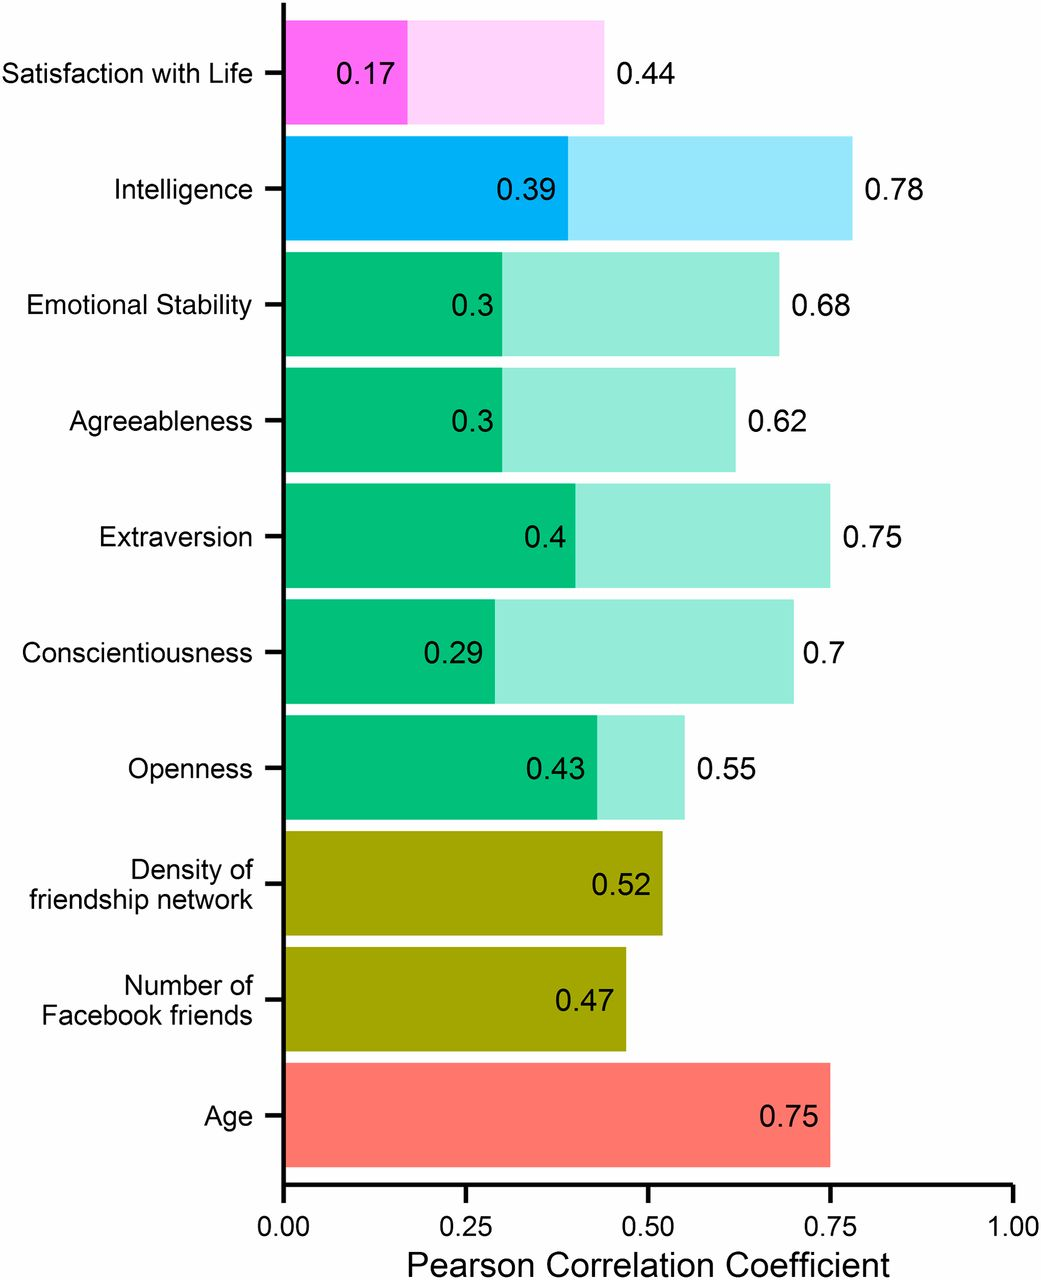
\includegraphics[width=0.33\textwidth,height=\textheight]{img/pnas.kosinski.1218772110fig03.jpeg}

}

\caption{\label{fig-pnas1}Prediction accuracy of regression for numeric
attributes and traits expressed by the Pearson correlation coefficient
between predicted and actual attribute values}

\end{figure}%

\section{Wetter in Deutschland}\label{wetter-in-deutschland}

\begin{example}[Wetterdaten]\protect\hypertarget{exm-wetterdaten}{}\label{exm-wetterdaten}

Nachdem Sie einige Zeit als Datenanalyst bei dem Online-Auktionshaus
gearbeitet haben, stand Ihnen der Sinn nach ewtas Abwechslung. Viel Geld
verdienen und Ruhm und Anerkennung sind ja schon ganz nett, aber dann
fiel Ihnen ein, dass Sie ja zu Generation Z gehören, und daher den
schnöden Mammon nicht so hoch schätzen sollten. Sie entschließen sich,
Ihre hochgeschätzten Analyse-Skills für etwas einzusetzen, das Ihnen
sinnvoll erscheint: Die Analyse des Klimawandels.

Beim \href{https://www.dwd.de/DE/Home/home_node.html}{Deutschen
Wetterdienst, DWD} haben Sie sich Wetterdaten von Deutschland
heruntergeladen. Nach etwas
\href{https://data-se.netlify.app/2022/07/24/preparing-german-weather-data/}{Datenjudo,
auf das wir hier nicht eingehen wollen} resultiert ein schöner
Datensatz, den Sie jetzt analysieren wollen\footnote{Temperatur: Grad
  Celcius, Niederschlag (\texttt{precip}) mm Niederschlag pro
  Quadratmeter}:

\begin{Shaded}
\begin{Highlighting}[]
\NormalTok{wetter\_path }\OtherTok{\textless{}{-}} \FunctionTok{paste0}\NormalTok{(}
  \StringTok{"https://raw.githubusercontent.com/sebastiansauer/"}\NormalTok{,}
  \StringTok{"Lehre/main/data/wetter{-}dwd/precip\_temp\_DWD.csv"}\NormalTok{)}

\NormalTok{wetter }\OtherTok{\textless{}{-}} \FunctionTok{read.csv}\NormalTok{(wetter\_path)}
\end{Highlighting}
\end{Shaded}

Ein \emph{Data-Dictionary} für den Datensatz können Sie
\href{https://raw.githubusercontent.com/sebastiansauer/Lehre/main/data/wetter-dwd/wetter-dwd-data-dict.md}{hier}
herunterladen.\footnote{\url{https://raw.githubusercontent.com/sebastiansauer/Lehre/main/data/wetter-dwd/wetter-dwd-data-dict.md}}

\begin{tcolorbox}[enhanced jigsaw, bottomtitle=1mm, title=\textcolor{quarto-callout-note-color}{\faInfo}\hspace{0.5em}{Hinweis}, toptitle=1mm, arc=.35mm, bottomrule=.15mm, breakable, colbacktitle=quarto-callout-note-color!10!white, left=2mm, colframe=quarto-callout-note-color-frame, colback=white, opacityback=0, titlerule=0mm, rightrule=.15mm, opacitybacktitle=0.6, leftrule=.75mm, toprule=.15mm, coltitle=black]

Ein \emph{Data-Dictionary} (Codebook) erklärt einen Datensatz. Oft
bedeutet das, das für jede Spalte der Datentabelle erklärt wird, was die
Spalte bedeutet.\(\square\)

\end{tcolorbox}

Hervorragend! An die Arbeit!

\end{example}

\subsection{metrische UV}\label{metrische-uv}

\subsubsection{Modell Wetter1}\label{modell-wetter1}

Sie stellen sich nun folgende Forschungsfrage:

\begin{quote}
{\emoji{teacher}} Um wieviel ist die Temperatur in Deutschland pro Jahr
gestiegen, wenn man die letzten ca. 100 Jahre betrachtet?
\end{quote}

Die Modellparameter von \texttt{lm\_wetter1} sind in
Tabelle~\ref{tbl-lm-wetter1} zu sehen.

\begin{Shaded}
\begin{Highlighting}[]
\NormalTok{lm\_wetter1 }\OtherTok{\textless{}{-}} \FunctionTok{lm}\NormalTok{(temp }\SpecialCharTok{\textasciitilde{}}\NormalTok{ year, }\AttributeTok{data =}\NormalTok{ wetter)}
\FunctionTok{parameters}\NormalTok{(lm\_wetter1)}
\end{Highlighting}
\end{Shaded}

\begin{longtable}[]{@{}
  >{\raggedright\arraybackslash}p{(\columnwidth - 10\tabcolsep) * \real{0.1690}}
  >{\centering\arraybackslash}p{(\columnwidth - 10\tabcolsep) * \real{0.1831}}
  >{\centering\arraybackslash}p{(\columnwidth - 10\tabcolsep) * \real{0.1408}}
  >{\centering\arraybackslash}p{(\columnwidth - 10\tabcolsep) * \real{0.2535}}
  >{\centering\arraybackslash}p{(\columnwidth - 10\tabcolsep) * \real{0.1408}}
  >{\centering\arraybackslash}p{(\columnwidth - 10\tabcolsep) * \real{0.1127}}@{}}

\caption{\label{tbl-lm-wetter1}Modellparameter von lm\_wetter1}

\tabularnewline

\toprule\noalign{}
\begin{minipage}[b]{\linewidth}\raggedright
Parameter
\end{minipage} & \begin{minipage}[b]{\linewidth}\centering
Coefficient
\end{minipage} & \begin{minipage}[b]{\linewidth}\centering
SE
\end{minipage} & \begin{minipage}[b]{\linewidth}\centering
95\% CI
\end{minipage} & \begin{minipage}[b]{\linewidth}\centering
t(28864)
\end{minipage} & \begin{minipage}[b]{\linewidth}\centering
p
\end{minipage} \\
\midrule\noalign{}
\endhead
\bottomrule\noalign{}
\endlastfoot
(Intercept) & -14.25 & 1.85 & (-17.87, -10.63) & -7.71 & \textless{}
.001 \\
year & 0.01 & 9.47e-04 & (9.80e-03, 0.01) & 12.30 & \textless{} .001 \\

\end{longtable}

Laut Ihrem Modell wurde es pro Jahr um 0.01 Grad wärmer, pro Jahrzehnt
also 0.1 und pro Jahrhundert 1 Grad.

\begin{quote}
{\emoji{student}} Das ist sicherlich nicht linear! Vermutlich ist die
Temperatur bis 1950 konstant geblieben und jetzt knallt sie durch die
Decke!
\end{quote}

\begin{quote}
{\emoji{teacher}} Mit der Ruhe, das schauen Sie sich später an.
\end{quote}

\subsubsection{Punkt-
vs.~Bereichsschätzung}\label{punkt--vs.-bereichsschuxe4tzung}

In tbl-lm-wetter1 finden sich zwei Arten von Information für den Wert
des Achsenabschnitts (b0) und des Regressionsgewichts von
\texttt{year}(b1):

\begin{enumerate}
\def\labelenumi{\arabic{enumi}.}
\item
  \emph{Punktschätzungen} In der Spalte \texttt{Coefficient} sehen Sie
  den ``Best-Guess'' für den entsprechenden Koeffizienten in der
  Population. Das is sozusagen der Wert für den sich das Modell
  festlegen würde, wenn es sonst nichts sagen dürfte.
\item
  \emph{Bereichschätzungen} Cleverer als Punktschätzungen sind
  Bereichsschätzungen (Intervallschätzungen): Hier wird ein Bereich
  plausibler Werte für den entsprechenden Wert angegeben. Der ``Bereich
  plausibler Werte'' wird auch als Konfidenzintervall (engl. confidence
  intervall, CI) bezeichnet. Entsprechend gibt \texttt{CI\_low} die
  Untergrenze des Bereichs plausibler Werte und \texttt{CI\_high} die
  Obergrenze aus. So können wir ablesen, dass das Regressionsgewicht von
  \texttt{year} irgendwo zwischen praktisch Null (0.009) und ca. 0.01
  Grad geschätzt wird.
\end{enumerate}

💡 Merke: Je schmaler das Konfidenzintervall, desto genauer wird der
Effekt geschätzt.

\subsubsection{Modell Wetter1a}\label{modell-wetter1a}

Das Modell \texttt{lm\_wetter1}, bzw. die Schätzungen zu den erwarteten
Werten, kann mich sich so ausgeben lassen, s.
Abbildung~\ref{fig-wetter1}, links. Allerdings sind das zu viele
Datenpunkte. Wir sollten es vielleicht anders visualisieren, s.
Abbildung~\ref{fig-wetter1}, rechts. Dazu aggregieren wir die Messwerte
eines Jahres zu jeweils einem Mittelwert.

\begin{Shaded}
\begin{Highlighting}[]
\NormalTok{wetter\_summ }\OtherTok{\textless{}{-}}
\NormalTok{  wetter }\SpecialCharTok{\%\textgreater{}\%} 
  \FunctionTok{group\_by}\NormalTok{(year) }\SpecialCharTok{\%\textgreater{}\%} 
  \FunctionTok{summarise}\NormalTok{(}\AttributeTok{temp =} \FunctionTok{mean}\NormalTok{(temp),}
            \AttributeTok{precip =} \FunctionTok{mean}\NormalTok{(precip))  }\CommentTok{\# precipitation: engl. für Niederschlag}
\end{Highlighting}
\end{Shaded}

Auf dieser Basis erstellen wir ein neues lineares Modell, s.
Tabelle~\ref{tbl-lm-wetter1a}.

\begin{Shaded}
\begin{Highlighting}[]
\NormalTok{lm\_wetter1a }\OtherTok{\textless{}{-}} \FunctionTok{lm}\NormalTok{(temp }\SpecialCharTok{\textasciitilde{}}\NormalTok{ year, }\AttributeTok{data =}\NormalTok{ wetter\_summ)}
\FunctionTok{parameters}\NormalTok{(lm\_wetter1a)}
\end{Highlighting}
\end{Shaded}

\begin{longtable}[]{@{}
  >{\raggedright\arraybackslash}p{(\columnwidth - 10\tabcolsep) * \real{0.1739}}
  >{\centering\arraybackslash}p{(\columnwidth - 10\tabcolsep) * \real{0.1884}}
  >{\centering\arraybackslash}p{(\columnwidth - 10\tabcolsep) * \real{0.1449}}
  >{\centering\arraybackslash}p{(\columnwidth - 10\tabcolsep) * \real{0.2609}}
  >{\centering\arraybackslash}p{(\columnwidth - 10\tabcolsep) * \real{0.1159}}
  >{\centering\arraybackslash}p{(\columnwidth - 10\tabcolsep) * \real{0.1159}}@{}}

\caption{\label{tbl-lm-wetter1a}Modellparameter von lm\_wetter1a}

\tabularnewline

\toprule\noalign{}
\begin{minipage}[b]{\linewidth}\raggedright
Parameter
\end{minipage} & \begin{minipage}[b]{\linewidth}\centering
Coefficient
\end{minipage} & \begin{minipage}[b]{\linewidth}\centering
SE
\end{minipage} & \begin{minipage}[b]{\linewidth}\centering
95\% CI
\end{minipage} & \begin{minipage}[b]{\linewidth}\centering
t(140)
\end{minipage} & \begin{minipage}[b]{\linewidth}\centering
p
\end{minipage} \\
\midrule\noalign{}
\endhead
\bottomrule\noalign{}
\endlastfoot
(Intercept) & -14.14 & 2.70 & (-19.48, -8.79) & -5.23 & \textless{}
.001 \\
year & 0.01 & 1.38e-03 & (8.86e-03, 0.01) & 8.38 & \textless{} .001 \\

\end{longtable}

\begin{Shaded}
\begin{Highlighting}[]
\FunctionTok{plot}\NormalTok{(}\FunctionTok{estimate\_relation}\NormalTok{(lm\_wetter1)) }
\FunctionTok{plot}\NormalTok{(}\FunctionTok{estimate\_relation}\NormalTok{(lm\_wetter1a))}
\end{Highlighting}
\end{Shaded}

\begin{figure}

\begin{minipage}{0.50\linewidth}

\centering{

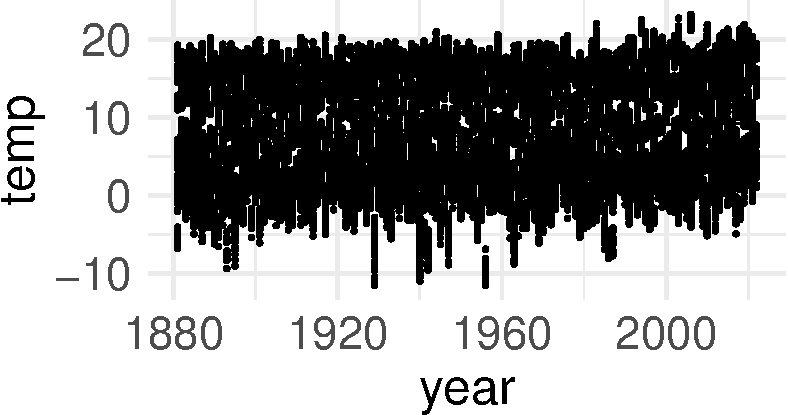
\includegraphics{090-regression2_files/figure-pdf/fig-wetter1-1.pdf}

}

\subcaption{\label{fig-wetter1-1}Jeder Punkt ist ein Tag (viel
Overplotting, wenig nützlich)}

\end{minipage}%
%
\begin{minipage}{0.50\linewidth}

\centering{

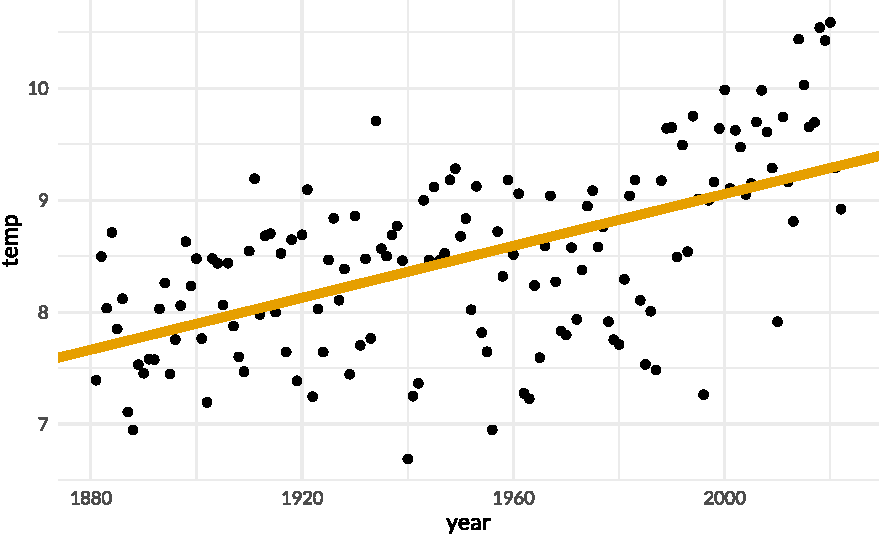
\includegraphics{090-regression2_files/figure-pdf/fig-wetter1-2.pdf}

}

\subcaption{\label{fig-wetter1-2}Jeder Punkt ist ein Jahr
(wetter\_summ)}

\end{minipage}%

\caption{\label{fig-wetter1}Die Veränderung der mittleren Temperatur in
Deutschland im Zeitverlauf (Datenquelle: DWD)}

\end{figure}%

\begin{quote}
{\emoji{student}} Moment mal, der Achsenabschnitt liegt bei -15 Grad!
Was soll das bitte bedeuten?
\end{quote}

\subsection{UV zentrieren}\label{uv-zentrieren}

Zur Erinnerung: Der Achsenabschnitt (\(\beta_0\); engl.
\emph{intercept}) ist definiert als der Y-Wert an der Stelle X=0, s.
\textbf{?@sec-interpret-reg-mod}.

In den Wetterdaten wäre Jahr=0 Christi Geburt. Da unsere
Wetteraufzeichnung gerade mal ca. 150 Jahre in die Vergangenheit reicht,
ist es vollkommen vermessen, dass Modell 2000 Jahre in die Vergangenheit
zu extraplieren, ganz ohne dass wir dafür Daten haben, s.
Abbildung~\ref{fig-extrapolation}.

\begin{figure}

\centering{

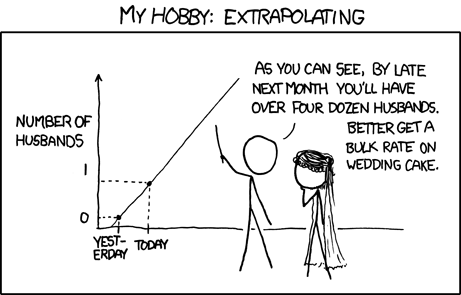
\includegraphics{img/extrapolating.png}

}

\caption{\label{fig-extrapolation}Du sollst nicht ein Modell weit
außerhalb seines Datenbereichs extrapolieren}

\end{figure}%

Sinnvoller ist es da, z.B. einen \emph{Referenzwert} festzulegen, etwa
1950. Wenn wir dann von allen Jahren 1950 abziehen, wird das Jahr 1950
zum neuen Jahr Null. Damit bezöge sich der Achsenabschnitt auf das Jahr
1950, was Sinn macht, denn für dieses Jahr haben wir Daten.

Hat man nicht einen bestimmten Wert, der sich als Referenzwert anbietet,
so ist es üblich, z.B. den Mittelwert (der UV) als Referenzwert zu
nehmen. Diese Transformation bezeichnet man als \emph{Zentrierung}
(engl. centering) der Daten.

So zentriert man eine Verteilung:

\begin{Shaded}
\begin{Highlighting}[]
\NormalTok{wetter }\OtherTok{\textless{}{-}}
\NormalTok{  wetter }\SpecialCharTok{\%\textgreater{}\%} 
  \FunctionTok{mutate}\NormalTok{(}\AttributeTok{year\_c =}\NormalTok{ year }\SpecialCharTok{{-}} \FunctionTok{mean}\NormalTok{(year))  }\CommentTok{\# "c" wie centered}
\end{Highlighting}
\end{Shaded}

Das mittlere Jahr in unserer Messwertereihe ist übrigens 1951:

\begin{Shaded}
\begin{Highlighting}[]
\NormalTok{wetter }\SpecialCharTok{\%\textgreater{}\%} 
  \FunctionTok{summarise}\NormalTok{(}\FunctionTok{mean}\NormalTok{(year))}
\end{Highlighting}
\end{Shaded}

\begin{longtable}[]{@{}r@{}}
\toprule\noalign{}
mean(year) \\
\midrule\noalign{}
\endhead
\bottomrule\noalign{}
\endlastfoot
1951.251 \\
\end{longtable}

Die Steigung (d.h. der Regressionskoeffizient für \texttt{year\_c})
bleibt unverändert, nur der Achsenabschnitt ändert sich, s.
Tabelle~\ref{tbl-lm_wetter1_zentriert}.

\begin{Shaded}
\begin{Highlighting}[]
\NormalTok{lm\_wetter1\_zentriert }\OtherTok{\textless{}{-}} \FunctionTok{lm}\NormalTok{(temp }\SpecialCharTok{\textasciitilde{}}\NormalTok{ year\_c, }\AttributeTok{data =}\NormalTok{ wetter)}
\FunctionTok{parameters}\NormalTok{(lm\_wetter1\_zentriert)}
\end{Highlighting}
\end{Shaded}

\begin{longtable}[]{@{}
  >{\raggedright\arraybackslash}p{(\columnwidth - 10\tabcolsep) * \real{0.1690}}
  >{\centering\arraybackslash}p{(\columnwidth - 10\tabcolsep) * \real{0.1831}}
  >{\centering\arraybackslash}p{(\columnwidth - 10\tabcolsep) * \real{0.1408}}
  >{\centering\arraybackslash}p{(\columnwidth - 10\tabcolsep) * \real{0.2535}}
  >{\centering\arraybackslash}p{(\columnwidth - 10\tabcolsep) * \real{0.1408}}
  >{\centering\arraybackslash}p{(\columnwidth - 10\tabcolsep) * \real{0.1127}}@{}}

\caption{\label{tbl-lm_wetter1_zentriert}Modellparameter von
lm\_wetter1\_zentriert}

\tabularnewline

\toprule\noalign{}
\begin{minipage}[b]{\linewidth}\raggedright
Parameter
\end{minipage} & \begin{minipage}[b]{\linewidth}\centering
Coefficient
\end{minipage} & \begin{minipage}[b]{\linewidth}\centering
SE
\end{minipage} & \begin{minipage}[b]{\linewidth}\centering
95\% CI
\end{minipage} & \begin{minipage}[b]{\linewidth}\centering
t(28864)
\end{minipage} & \begin{minipage}[b]{\linewidth}\centering
p
\end{minipage} \\
\midrule\noalign{}
\endhead
\bottomrule\noalign{}
\endlastfoot
(Intercept) & 8.49 & 0.04 & (8.42, 8.57) & 219.43 & \textless{} .001 \\
year c & 0.01 & 9.47e-04 & (9.80e-03, 0.01) & 12.30 & \textless{}
.001 \\

\end{longtable}

Jetzt ist die Interpretation des Achsenabschnitts komfortabel: Im Jahr
1951 (x=0) lag die mittlere Temperatur in Deutschland (laut DWD) bei ca.
8.5 Grad Celcius. Die Regressionsgleichung lautet:
\texttt{temp\_pred\ =\ 8.49\ +\ 0.01*year\_c}. In Worten: Wir sagen eine
Temperatur vorher, die sich als Summe von 8.49 Grad plus 0.01 mal das
Jahr (in zentrierter Form) berechnet.

\begin{tcolorbox}[enhanced jigsaw, bottomtitle=1mm, title=\textcolor{quarto-callout-important-color}{\faExclamation}\hspace{0.5em}{Referenzwert entspricht Null}, toptitle=1mm, arc=.35mm, bottomrule=.15mm, breakable, colbacktitle=quarto-callout-important-color!10!white, left=2mm, colframe=quarto-callout-important-color-frame, colback=white, opacityback=0, titlerule=0mm, rightrule=.15mm, opacitybacktitle=0.6, leftrule=.75mm, toprule=.15mm, coltitle=black]

Der Referenzwert bzw. der Wert der Referenzgruppe entspricht dem Y-Wert
bei x=0 im Regressionsmodell.\(\square\)

\end{tcolorbox}

Wie gut erklärt unser Modell die Daten?

\begin{Shaded}
\begin{Highlighting}[]
\FunctionTok{r2}\NormalTok{(lm\_wetter1\_zentriert)  }\CommentTok{\# aus \textasciigrave{}\{easystats\}\textasciigrave{}}
\DocumentationTok{\#\# \# R2 for Linear Regression}
\DocumentationTok{\#\#        R2: 0.005}
\DocumentationTok{\#\#   adj. R2: 0.005}
\end{Highlighting}
\end{Shaded}

Viel Varianz des Wetters erklärt das Modell mit
\texttt{year\_c}\footnote{\texttt{year} und \texttt{year\_c} sind gleich
  stark mit \texttt{temp} korreliert, daher wird sich die Modellgüte
  nicht unterscheiden.} aber nicht. Macht auch Sinn: Abgesehen von der
Jahreszahl spielt z.B. die Jahreszeit eine große Rolle für die
Temperatur. Das haben wir nicht berücksichtigt.

\begin{quote}
{\emoji{student}} Wie warm ist es laut unserem Modell dann im Jahr 2051?
\end{quote}

\begin{Shaded}
\begin{Highlighting}[]
\FunctionTok{predict}\NormalTok{(lm\_wetter1\_zentriert, }\AttributeTok{newdata =} \FunctionTok{tibble}\NormalTok{(}\AttributeTok{year\_c =} \DecValTok{100}\NormalTok{))}
\DocumentationTok{\#\#       1 }
\DocumentationTok{\#\# 9.65775}
\end{Highlighting}
\end{Shaded}

\begin{quote}
{\emoji{student}} Moment! Die Vorhersage ist doch Quatsch! Schon im Jahr
2022 lag die Durchschnittstemperatur bei 10,5° Celcius.\footnote{\href{https://www.umweltbundesamt.de/daten/klima/trends-der-lufttemperatur\#steigende-durchschnittstemperaturen-weltweit}{Quelle:
  Umweltbundesamt}}
\end{quote}

\begin{quote}
{\emoji{teacher}} Wir brauchen ein besseres Modell! Zum Glück haben wir
ambitionierte Nachwuchs-Wissenschaftler:innen.
\end{quote}

\subsection{Binäre UV}\label{binuxe4re-uv}

\begin{definition}[Binäre
Variable]\protect\hypertarget{def-binvar}{}\label{def-binvar}

Eine \emph{binäre} UV, auch \emph{Indikatorvariable} oder
\emph{Dummyvariable} genannt, hat nur zwei Ausprägungen: 0 und
1.\(\square\)

\end{definition}

\begin{example}[Binäre
Variablen]\protect\hypertarget{exm-bin}{}\label{exm-bin}

Das sind zum Beispiel \emph{weiblich} mit den Ausprägungen \texttt{0}
(nein) und \texttt{1} (ja) oder \emph{before\_1950} mit \texttt{1} für
Jahre früher als 1950 und \texttt{0} ansonsten.\(\square\)

\end{example}

\begin{example}[]\protect\hypertarget{exm-binuv}{}\label{exm-binuv}

Hier interessiert Sie folgende Forschungsfrage:

\begin{quote}
{\emoji{student}} Ob es in der zweiten Hälfte des 20. Jahrhunderts wohl
wärmer warm, im Durchschnitt, als vorher?\(\square\)
\end{quote}

\end{example}

Aber wie erstellen Sie eine Variable \texttt{after\_1950}, um die zweite
Hälfte des 20. Jahrhunderts (und danach) zu fassen? Nach einigem
Überlegen kommen Sie auf die Idee, das vektorisierte Rechnen von R (s.
\textbf{?@sec-veccalc}) auszunutzen:

\begin{Shaded}
\begin{Highlighting}[]
\NormalTok{year }\OtherTok{\textless{}{-}} \FunctionTok{c}\NormalTok{(}\DecValTok{1940}\NormalTok{, }\DecValTok{1950}\NormalTok{, }\DecValTok{1960}\NormalTok{)}
\NormalTok{after\_1950 }\OtherTok{\textless{}{-}}\NormalTok{ year }\SpecialCharTok{\textgreater{}} \DecValTok{1950}  \CommentTok{\# prüfe ob as Jahr größer als 1950 ist}
\NormalTok{after\_1950}
\DocumentationTok{\#\# [1] FALSE FALSE  TRUE}
\end{Highlighting}
\end{Shaded}

Die ersten zwei Jahre von \texttt{year} sind nicht größer als 1950, das
dritte schon.

Ja, so könnte das klappen! Diese Syntax übertragen Sie auf Ihre
\texttt{wetter}-Daten:

\begin{Shaded}
\begin{Highlighting}[]
\NormalTok{wetter }\OtherTok{\textless{}{-}}
\NormalTok{  wetter }\SpecialCharTok{\%\textgreater{}\%} 
  \FunctionTok{mutate}\NormalTok{(}\AttributeTok{after\_1950 =}\NormalTok{ year }\SpecialCharTok{\textgreater{}} \DecValTok{1950}\NormalTok{) }\SpecialCharTok{\%\textgreater{}\%} 
  \FunctionTok{filter}\NormalTok{(region }\SpecialCharTok{!=} \StringTok{"Deutschland"}\NormalTok{)  }\CommentTok{\# ohne Daten für Gesamt{-}Deutschland}
\end{Highlighting}
\end{Shaded}

Scheint zu klappen!

Jetzt ein lineares Modell dazu berechnen:

\begin{Shaded}
\begin{Highlighting}[]
\NormalTok{lm\_wetter\_bin\_uv }\OtherTok{\textless{}{-}} \FunctionTok{lm}\NormalTok{(temp }\SpecialCharTok{\textasciitilde{}}\NormalTok{ after\_1950, }\AttributeTok{data =}\NormalTok{ wetter)}
\end{Highlighting}
\end{Shaded}

Die Parameter des Modells lassen darauf schließen, dass es tatsächlich
wärmer war nach 1950, und zwar im Schnitt offenbar ein gutes halbes
Grad, s. Abbildung~\ref{fig-wetter2}.

\begin{figure}

\begin{minipage}{0.50\linewidth}

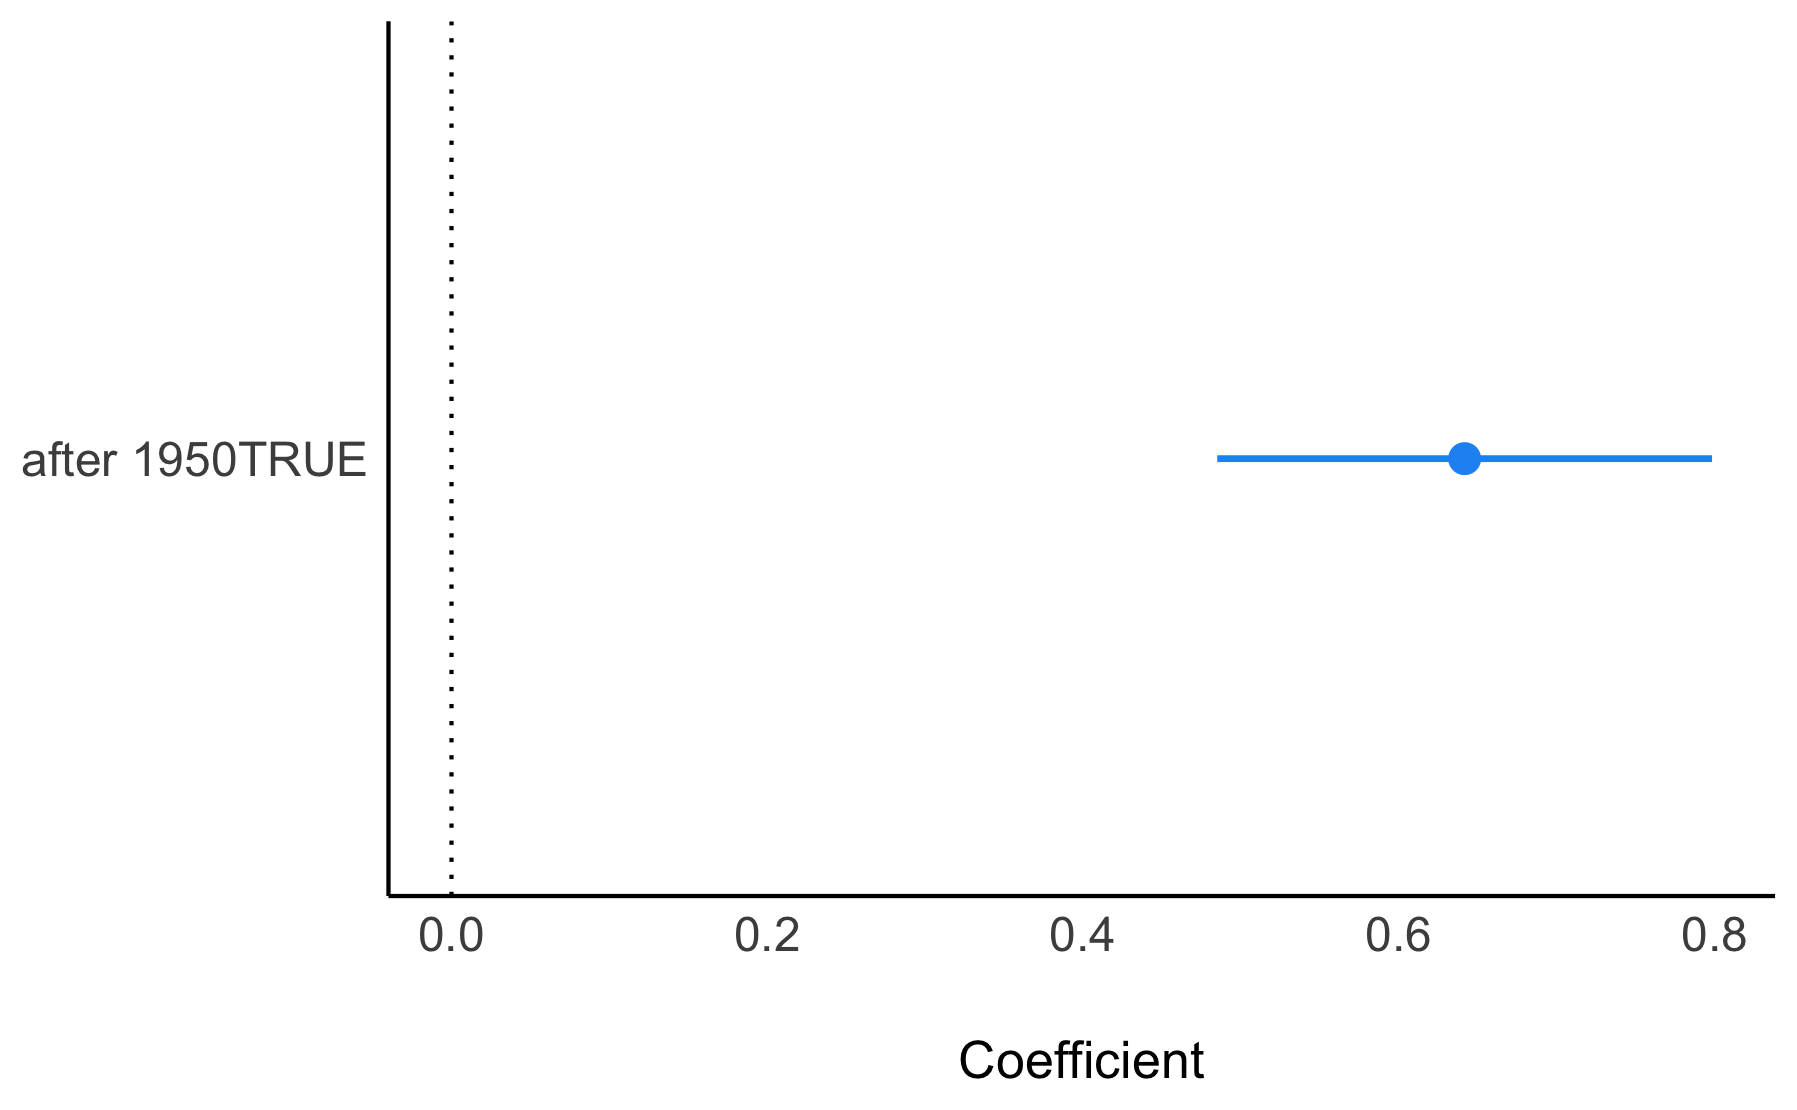
\includegraphics{img/fig-lm-wetter-bin-uv.png}

\subcaption{\label{}Der Schätzbereich für den Parameter reicht von ca.
0.5 bis 0.8 Grad Unterschied}
\end{minipage}%
%
\begin{minipage}{0.50\linewidth}

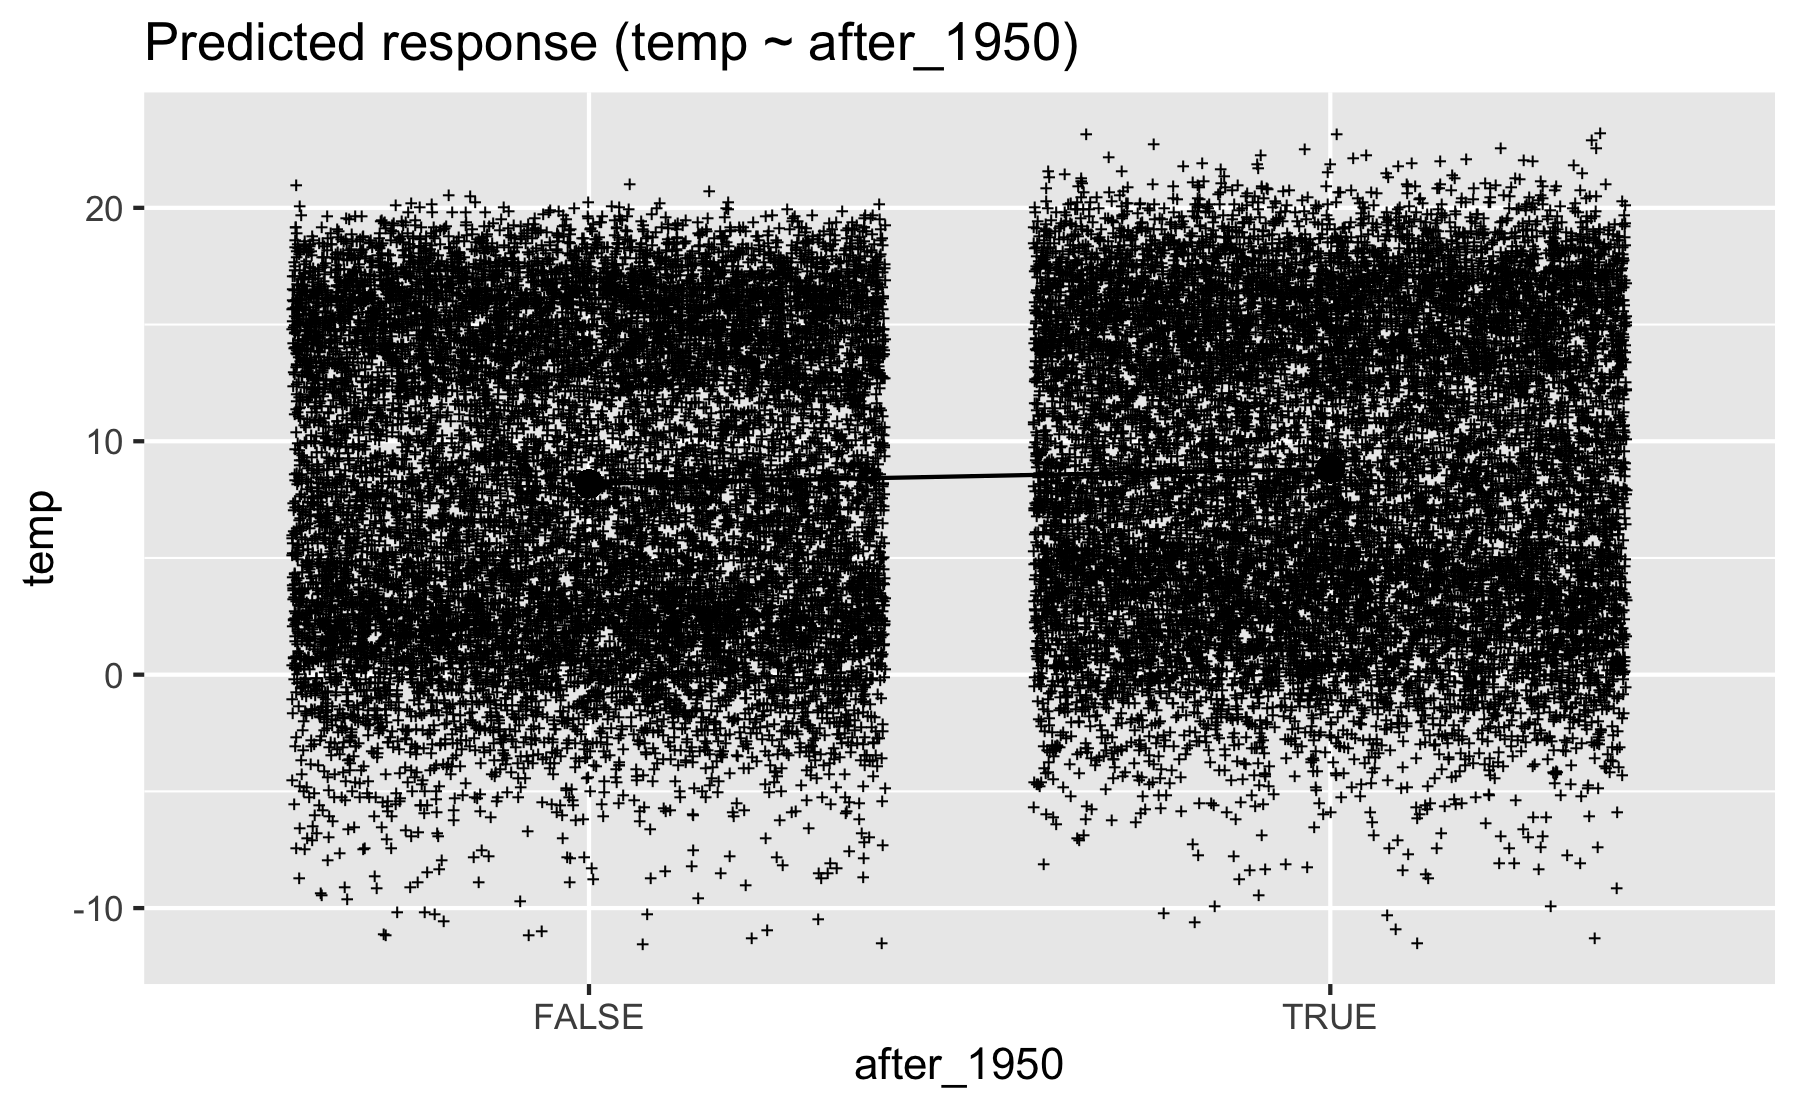
\includegraphics{img/fig-temp-after1950.png}

\subcaption{\label{}Wie man sieht, überlappen die Temperaturen dennoch
beträchtlich; aufgrund des starken Overplotting ist dieses Diagramm
alles andere als ideal}
\end{minipage}%

\caption{\label{fig-wetter2}Modell
\texttt{temp\ \textasciitilde{}\ after\_1950}}

\end{figure}%

Leider zeigt ein Blick zum \texttt{r2}, dass die Vorhersagegüte des
Modells zu wünschen übrig lässt\footnote{\texttt{r2(lm\_wetter\_bin\_uv)}}.
\(\square\)

\begin{tcolorbox}[enhanced jigsaw, bottomtitle=1mm, title=\textcolor{quarto-callout-important-color}{\faExclamation}\hspace{0.5em}{Lineare Modelle verkraften nur metrische Variablen}, toptitle=1mm, arc=.35mm, bottomrule=.15mm, breakable, colbacktitle=quarto-callout-important-color!10!white, left=2mm, colframe=quarto-callout-important-color-frame, colback=white, opacityback=0, titlerule=0mm, rightrule=.15mm, opacitybacktitle=0.6, leftrule=.75mm, toprule=.15mm, coltitle=black]

Um die Koeffizienten eines linearen Modells auszurechnen, benötigt man
eine metrische X- und eine metrische Y-Variable. Hier haben wir aber
keine richtige metrische X-Variable\footnotemark{}, sondern eine
\emph{logische} Variable mit den Werten \texttt{TRUE} und
\texttt{FALSE}.\(\square\)

\end{tcolorbox}

\footnotetext{UV}

Um die X-Variable in eine metrische Variable umzuwandeln, gibt es einen
einfachen Trick, den R für uns ohne viel Ankündigung durchführt:
Umwandling in mehrere binäre Variablen.

Hat ein nominaler Prädiktor zwei Stufen, so überführt\footnote{synonym:
  transformiert} \texttt{lm()} diese Variable in eine binäre Variable.
Da eine binäre Variable metrisch ist, kann die Regression in gewohnter
Weise durchgeführt werden. Wenn Sie die Ausgabe der Parameter
betrachten, so sehen Sie die neu erstellte binäre Variable. Man beachte,
dass der ursprüngliche Datensatz nicht geändert wird, nur während der
Analyse von \texttt{lm} wird die Umwandlung der Variable \footnote{Transformation}
durchgeführt.

\begin{quote}
{\emoji{robot}} Eine \texttt{1} kannst du als ``Ja! Richtig!'' verstehen
und eine\texttt{0} als ``Nein! Falsch!''
\end{quote}

\texttt{after\_1950} wird in eine Indikatorvariable umgewandelt:

\begin{figure}

\begin{minipage}{0.40\linewidth}

\begin{longtable}[]{@{}rl@{}}
\toprule\noalign{}
id & after\_1950 \\
\midrule\noalign{}
\endhead
\bottomrule\noalign{}
\endlastfoot
1 & TRUE \\
2 & FALSE \\
\end{longtable}

\end{minipage}%
%
\begin{minipage}{0.20\linewidth}
\(\qquad \rightarrow\)\end{minipage}%
%
\begin{minipage}{0.40\linewidth}

\begin{longtable}[]{@{}rr@{}}
\toprule\noalign{}
id & after\_1950TRUE \\
\midrule\noalign{}
\endhead
\bottomrule\noalign{}
\endlastfoot
1 & 1 \\
2 & 0 \\
\end{longtable}

\end{minipage}%

\end{figure}%

\begin{example}[Beispiel: `Geschlecht' in eine binäre Variable
umwandeln.]\protect\hypertarget{exm-bin-trans}{}\label{exm-bin-trans}

Angenommen wir haben eine Variable \texttt{geschlecht} mit den zwei
Stufen \texttt{Frau} und \texttt{Mann} und wollen diese in eine
Indikatorvariable umwandeln. Da ``Frau'' alphabetisch vor ``Mann''
kommt, nimmt R ``Frau'' als \emph{erste} Stufe bzw. als
\emph{Referenzgruppe}. ``Mann'' ist dann die zweite Stufe, die in der
Regression dann in Bezug zur Referenzgruppe gesetzt wird. \texttt{lm}
wandelt uns diese Variable in \texttt{geschlechtMann} um mit den zwei
Stufen \texttt{0} (kein Mann, also Frau) und \texttt{1}
(Mann).\(\square\)

\end{example}

\begin{figure}

\begin{minipage}{0.40\linewidth}

\begin{longtable}[]{@{}rl@{}}
\toprule\noalign{}
id & geschlecht \\
\midrule\noalign{}
\endhead
\bottomrule\noalign{}
\endlastfoot
1 & Mann \\
2 & Frau \\
\end{longtable}

\end{minipage}%
%
\begin{minipage}{0.20\linewidth}
\(\qquad \rightarrow\)\end{minipage}%
%
\begin{minipage}{0.40\linewidth}

\begin{longtable}[]{@{}rr@{}}
\toprule\noalign{}
id & geschlechtMann \\
\midrule\noalign{}
\endhead
\bottomrule\noalign{}
\endlastfoot
1 & 1 \\
2 & 0 \\
\end{longtable}

\end{minipage}%

\end{figure}%

Ein lineares Modell mit binärer UV ist nichts anderes die Differenz der
Gruppenmittelwerte zu berechnen:

\begin{Shaded}
\begin{Highlighting}[]
\NormalTok{wetter }\SpecialCharTok{\%\textgreater{}\%} 
  \FunctionTok{group\_by}\NormalTok{(after\_1950) }\SpecialCharTok{\%\textgreater{}\%} 
  \FunctionTok{summarise}\NormalTok{(}\AttributeTok{temp\_mean =} \FunctionTok{mean}\NormalTok{(temp))}
\end{Highlighting}
\end{Shaded}

\begin{longtable}[]{@{}lr@{}}
\toprule\noalign{}
after\_1950 & temp\_mean \\
\midrule\noalign{}
\endhead
\bottomrule\noalign{}
\endlastfoot
FALSE & 8.175287 \\
TRUE & 8.816761 \\
\end{longtable}

Die Interpretation eines linearen Modells mit binärer UV veranschaulicht
Abbildung~\ref{fig-binvar}: Der Achsenabschnitt (b0) entspricht dem
Mittelwert der 1. Gruppe. Der Mittelwert der 2. Gruppe entspricht der
\emph{Summe} aus Achsenabschnitt und dem Koeffizienten der zweiten
Gruppe. (Abbildung~\ref{fig-binvar} zeigt nur die Daten für den Monat
Juli im Bundesland Bayern, der Einfachheit und Übersichtlichkeit
halber.)

\begin{figure}

\centering{

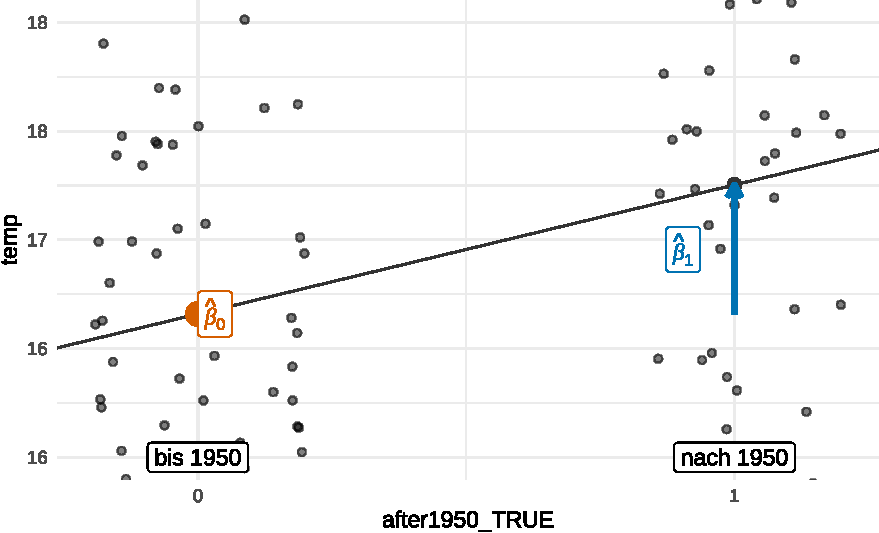
\includegraphics{090-regression2_files/figure-pdf/fig-binvar-1.pdf}

}

\caption{\label{fig-binvar}Sinnbild zur Interpretation eines linearen
Modells mit binärer UV (reingezoomt, um den Mittelwertsunterschied
hervorzuheben)}

\end{figure}%

Fassen wir die Interpretation der Koeffizienten für das Modell mit
binärer UV zusammen:

\begin{enumerate}
\def\labelenumi{\arabic{enumi}.}
\tightlist
\item
  Mittelwert der 1. Gruppe (bis 1950): {Achsenabschnitt (b0)}
\item
  Mittelwert der 2. Gruppe (nach 1950): {Achsenabschnitt (b0)} +
  {Steigung der Regressionsgeraden (b1)}
\end{enumerate}

Für die Modellwerte \(\color{modelcol}{\hat{y}}\) gilt also:

\begin{itemize}
\item
  Temperatur laut Modell bis 1950:
  \(\color{modelcol}{\hat{y}} = \color{beta0col}{\beta_0} = 17.7\)
\item
  Temperatur laut Modell bis 1950:
  \(\color{modelcol}{\hat{y}} = \color{beta0col}{\beta_0} +  \color{beta1col}{\beta_1}= \color{beta0col}{17.7} + \color{beta1col}{0.6} = 18.3\)
\end{itemize}

\begin{tcolorbox}[enhanced jigsaw, bottomtitle=1mm, title=\textcolor{quarto-callout-note-color}{\faInfo}\hspace{0.5em}{Hinweis}, toptitle=1mm, arc=.35mm, bottomrule=.15mm, breakable, colbacktitle=quarto-callout-note-color!10!white, left=2mm, colframe=quarto-callout-note-color-frame, colback=white, opacityback=0, titlerule=0mm, rightrule=.15mm, opacitybacktitle=0.6, leftrule=.75mm, toprule=.15mm, coltitle=black]

Bei \emph{nominalen} (und auch bei \emph{binären}) Variablen ist
\(\color{beta1col}{\beta_1}\) ein \emph{Schalter}; bei \emph{metrischen}
Variablen ein \emph{Dimmer}.\footnotemark{} \(\square\)

\end{tcolorbox}

\footnotetext{Ich danke Karsten Lübke für diese Idee.}

\subsection{Nominale UV}\label{nominale-uv}

In diesem Abschnitt betrachten wir ein lineare Modell\footnote{für uns
  synonym: Regressionsmodell} mit einer mehrstufigen\footnote{drei oder
  mehr Stufen bzw. Ausprägungen} (nominalskalierten) UV.\footnote{So ein
  Modell ist von den Ergebnissen her praktisch identisch zu einer
  einfachen \emph{Varianzanalyse}.}

\begin{example}[]\protect\hypertarget{exm-wetter2}{}\label{exm-wetter2}

Ob es wohl substanzielle\footnote{wie könnte man dieses Wort eigentlich
  definieren?} Temperaturunterschiede zwischen den Bundesländern gibt?

\end{example}

Befragen wir dazu ein lineares Modell, s.
Tabelle~\ref{tbl-lm_wetter_region}.

\begin{Shaded}
\begin{Highlighting}[]
\NormalTok{lm\_wetter\_region }\OtherTok{\textless{}{-}} \FunctionTok{lm}\NormalTok{(temp }\SpecialCharTok{\textasciitilde{}}\NormalTok{ region, }\AttributeTok{data =}\NormalTok{ wetter)}
\FunctionTok{parameters}\NormalTok{(lm\_wetter\_region)}
\end{Highlighting}
\end{Shaded}

\begin{longtable}[]{@{}
  >{\raggedright\arraybackslash}p{(\columnwidth - 10\tabcolsep) * \real{0.4176}}
  >{\centering\arraybackslash}p{(\columnwidth - 10\tabcolsep) * \real{0.1429}}
  >{\centering\arraybackslash}p{(\columnwidth - 10\tabcolsep) * \real{0.0659}}
  >{\centering\arraybackslash}p{(\columnwidth - 10\tabcolsep) * \real{0.1758}}
  >{\centering\arraybackslash}p{(\columnwidth - 10\tabcolsep) * \real{0.1099}}
  >{\centering\arraybackslash}p{(\columnwidth - 10\tabcolsep) * \real{0.0879}}@{}}

\caption{\label{tbl-lm_wetter_region}Modellparameter für
lm\_wetter\_region}

\tabularnewline

\toprule\noalign{}
\begin{minipage}[b]{\linewidth}\raggedright
Parameter
\end{minipage} & \begin{minipage}[b]{\linewidth}\centering
Coefficient
\end{minipage} & \begin{minipage}[b]{\linewidth}\centering
SE
\end{minipage} & \begin{minipage}[b]{\linewidth}\centering
95\% CI
\end{minipage} & \begin{minipage}[b]{\linewidth}\centering
t(27152)
\end{minipage} & \begin{minipage}[b]{\linewidth}\centering
p
\end{minipage} \\
\midrule\noalign{}
\endhead
\bottomrule\noalign{}
\endlastfoot
(Intercept) & 8.25 & 0.16 & (7.93, 8.56) & 51.62 & \textless{} .001 \\
region (Bayern) & -0.63 & 0.23 & (-1.07, -0.19) & -2.79 & 0.005 \\
region (Brandenburg) & 0.57 & 0.23 & (0.13, 1.02) & 2.53 & 0.011 \\
region (Brandenburg/Berlin) & 0.58 & 0.23 & (0.14, 1.03) & 2.59 &
0.010 \\
region (Hessen) & 0.11 & 0.23 & (-0.33, 0.56) & 0.51 & 0.612 \\
region (Mecklenburg-Vorpommern) & 0.08 & 0.23 & (-0.37, 0.52) & 0.34 &
0.732 \\
region (Niedersachsen) & 0.52 & 0.23 & (0.07, 0.96) & 2.29 & 0.022 \\
region (Niedersachsen/Hamburg/Bremen) & 0.52 & 0.23 & (0.08, 0.96) &
2.31 & 0.021 \\
region (Nordrhein-Westfalen) & 0.80 & 0.23 & (0.35, 1.24) & 3.53 &
\textless{} .001 \\
region (Rheinland-Pfalz) & 0.46 & 0.23 & (0.02, 0.90) & 2.03 & 0.042 \\
region (Saarland) & 0.71 & 0.23 & (0.27, 1.16) & 3.16 & 0.002 \\
region (Sachsen) & -0.04 & 0.23 & (-0.48, 0.40) & -0.18 & 0.853 \\
region (Sachsen-Anhalt) & 0.55 & 0.23 & (0.11, 1.00) & 2.45 & 0.014 \\
region (Schleswig-Holstein) & 0.17 & 0.23 & (-0.27, 0.62) & 0.76 &
0.446 \\
region (Thueringen) & -0.48 & 0.23 & (-0.92, -0.03) & -2.11 & 0.035 \\
region (Thueringen/Sachsen-Anhalt) & 0.10 & 0.23 & (-0.34, 0.54) & 0.43
& 0.664 \\

\end{longtable}

Hat die nominalskalierte UV mehr als zwei Stufen, so transformiert
\texttt{lm} sie in mehr als eine Indikatorvariablen um. Genauer gesagt
ist es immer eine Indikatorvariablen weniger als es Stufen in der
nominalskalierten Variablen gibt.

Betrachten wir ein einfaches Beispiel, eine Tabelle mit der Spalte
\texttt{Bundesland} -- aus Gründen der Einfachheit hier nur mit
\emph{drei} Bundesländern. Damit \texttt{lm} arbeiten kann, wird
\texttt{Bundesland} in \emph{zwei} Indikatorvariablen umgewandelt:

\begin{figure}

\begin{minipage}{0.40\linewidth}

\begin{longtable}[]{@{}rl@{}}
\toprule\noalign{}
id & Bundesland \\
\midrule\noalign{}
\endhead
\bottomrule\noalign{}
\endlastfoot
1 & BaWü \\
2 & Bayern \\
3 & Brandenburg \\
\end{longtable}

\end{minipage}%
%
\begin{minipage}{0.20\linewidth}
\(\qquad \rightarrow\)\end{minipage}%
%
\begin{minipage}{0.40\linewidth}

\begin{longtable}[]{@{}rrr@{}}
\toprule\noalign{}
id & BL\_Bayern & BL\_Bra \\
\midrule\noalign{}
\endhead
\bottomrule\noalign{}
\endlastfoot
1 & 0 & 0 \\
2 & 1 & 0 \\
3 & 0 & 1 \\
\end{longtable}

\end{minipage}%

\end{figure}%

Auch im Fall mehrerer Ausprägungen einer nominalen Variablen gilt die
gleiche Logik der Interpretation wie bei binären Variablen:

\begin{enumerate}
\def\labelenumi{\arabic{enumi}.}
\tightlist
\item
  Mittelwert der 1. Gruppe: Achsenabschnitt (b0)
\item
  Mittelwert der 2. Gruppe: Achsenabschnitt (b0) + Steigung der 1.
  Regressionsgeraden (b1)
\item
  Mittelwert der 2. Gruppe: Achsenabschnitt (b0) + Steigung der 2.
  Regressionsgeraden (b2)
\item
  usw.
\end{enumerate}

Es kann nervig sein, dass das Bundesland, welches als
\emph{Referenzgruppe} (sprich als Gruppe des Achsenabschnitts ausgewählt
wurde) nicht explizit in der Ausgabe angegeben ist. Der Wert der
Referenzgruppe findet seinen Niederschlag im Achsenabschnitt.

\begin{tcolorbox}[enhanced jigsaw, bottomtitle=1mm, title=\textcolor{quarto-callout-note-color}{\faInfo}\hspace{0.5em}{Hinweis}, toptitle=1mm, arc=.35mm, bottomrule=.15mm, breakable, colbacktitle=quarto-callout-note-color!10!white, left=2mm, colframe=quarto-callout-note-color-frame, colback=white, opacityback=0, titlerule=0mm, rightrule=.15mm, opacitybacktitle=0.6, leftrule=.75mm, toprule=.15mm, coltitle=black]

Bei einer Variable vom Typ \texttt{character} wählt R den alphabetisch
ersten Wert als Referenzgruppe für ein lineares Modell aus. Bei einer
Variable vom Typ \texttt{factor} ist die Reihenfolge bereits festgelegt,
vgl. Kapitel~\ref{sec-faktorvar}. Der Mittelwert dieser Gruppe
entspricht dem Achsenabschnitt. \(\square\)

\end{tcolorbox}

\begin{example}[Achsenabschnitt in
wetter\_lm2]\protect\hypertarget{exm-bawü}{}\label{exm-bawü}

Da Baden-Württemberg das alphabetisch erste Bundesland ist, wird es von
R als Referenzgruppe ausgewählt, dessen Mittelwert als Achsenabschnitt
im linearen Modell hergenommen wird.\(\square\)

\end{example}

Am einfachsten verdeutlicht sich \texttt{lm\_wetter\_region} vielleicht
mit einem Diagramm, s. Abbildung~\ref{fig-bin-nom}.

\begin{figure}

\centering{

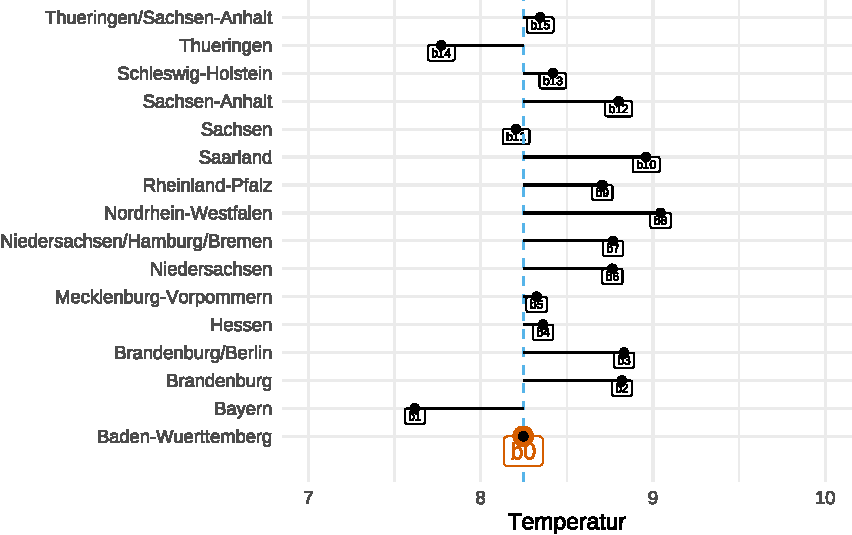
\includegraphics{090-regression2_files/figure-pdf/fig-bin-nom-1.pdf}

}

\caption{\label{fig-bin-nom}Sinnbild zur Interpretation eines linearen
Modells mit nominaler UV (reingezoomt, um den Mittelwertsunterschied
hervorzuheben). Die Achsen wurden um 90° gedreht, damit man die Namen
der Bundesländer besser lessen kann.}

\end{figure}%

\begin{example}[Niederschlagsmenge im Vergleich der
Monate]\protect\hypertarget{exm-months}{}\label{exm-months}

Eine weitere Forschungsfrage, die Sie nicht außer acht lassen wollen,
ist die Frage nach den jahreszeitlichen Unterschieden im Niederschlag
(engl. precipitation). Los R, rechnen!

\begin{quote}
{\emoji{robot}} Endlich geht's weiter! Ergebnisse in
Tabelle~\ref{tbl-lm_wetter-month}! \(\square\)
\end{quote}

\end{example}

\begin{Shaded}
\begin{Highlighting}[]
\NormalTok{lm\_wetter\_month }\OtherTok{\textless{}{-}} \FunctionTok{lm}\NormalTok{(precip }\SpecialCharTok{\textasciitilde{}}\NormalTok{ month, }\AttributeTok{data =}\NormalTok{ wetter)}
\FunctionTok{parameters}\NormalTok{(lm\_wetter\_month)}
\end{Highlighting}
\end{Shaded}

\begin{longtable}[]{@{}lccccc@{}}

\caption{\label{tbl-lm_wetter-month}Modellparameter für
lm\_wetter\_month}

\tabularnewline

\toprule\noalign{}
Parameter & Coefficient & SE & 95\% CI & t(27166) & p \\
\midrule\noalign{}
\endhead
\bottomrule\noalign{}
\endlastfoot
(Intercept) & 53.27 & 0.41 & (52.46, 54.08) & 128.76 & \textless{}
.001 \\
month & 1.14 & 0.06 & (1.03, 1.25) & 20.29 & \textless{} .001 \\

\end{longtable}

Ja, da scheint es deutliche Unterschied im Niederschlag zu geben. Wir
brauchen ein Diagramm zur Verdeutlichung, s.
Abbildung~\ref{fig-wetter-month}, links.\footnote{\texttt{plot(estimate\_expectation(lm\_wetter\_month)}}
Oh nein: R betrachtet \texttt{month} als numerische Variable! Aber
``Monat'' bzw. ``Jahreszeit'' sollte nominal sein.

\begin{quote}
{\emoji{robot}} Aber \texttt{month} ist als Zahl in der Tabelle
hinterlegt. Jede ehrliche Maschine verarbeitet eine Zahl als Zahl, ist
doch klar!
\end{quote}

\begin{quote}
{\emoji{woman}} Okay, R, wir müssen \texttt{month} in eine nominale Zahl
transformieren. Wie geht das?
\end{quote}

\begin{quote}
{\emoji{robot}} Dazu kannst du den Befehl \texttt{factor} nehmen. Damit
wandelst du eine numerische Variable in eine nominalskalierte Variable
(Faktorvariable) um. Faktisch heißt das, dass dann eine Zahl als Text
gesehen wird.
\end{quote}

\begin{example}[]\protect\hypertarget{exm-factor}{}\label{exm-factor}

Transformiert man \texttt{42} mit \texttt{factor}, so wird aus
\texttt{42} \texttt{"42"}. Aus der Zahl wird ein Text. Alle metrischen
Eigenschaften gehen verloren; die Variable ist jetzt auf nominalen
Niveau.\(\square\)

\end{example}

\begin{Shaded}
\begin{Highlighting}[]
\NormalTok{wetter }\OtherTok{\textless{}{-}}
\NormalTok{  wetter }\SpecialCharTok{\%\textgreater{}\%} 
  \FunctionTok{mutate}\NormalTok{(}\AttributeTok{month\_factor =} \FunctionTok{factor}\NormalTok{(month))}
\end{Highlighting}
\end{Shaded}

Jetzt berechnen wir mit der faktorisierten Variablen ein lineares
Modell, s. Tabelle~\ref{tbl-lm_wetter_month_factor}.

\begin{Shaded}
\begin{Highlighting}[]
\NormalTok{lm\_wetter\_month\_factor }\OtherTok{\textless{}{-}} \FunctionTok{lm}\NormalTok{(precip }\SpecialCharTok{\textasciitilde{}}\NormalTok{ month\_factor, }\AttributeTok{data =}\NormalTok{ wetter)}
\FunctionTok{parameters}\NormalTok{(lm\_wetter\_month\_factor)}
\end{Highlighting}
\end{Shaded}

\begin{longtable}[]{@{}
  >{\raggedright\arraybackslash}p{(\columnwidth - 10\tabcolsep) * \real{0.2500}}
  >{\centering\arraybackslash}p{(\columnwidth - 10\tabcolsep) * \real{0.1806}}
  >{\centering\arraybackslash}p{(\columnwidth - 10\tabcolsep) * \real{0.0833}}
  >{\centering\arraybackslash}p{(\columnwidth - 10\tabcolsep) * \real{0.2361}}
  >{\centering\arraybackslash}p{(\columnwidth - 10\tabcolsep) * \real{0.1389}}
  >{\centering\arraybackslash}p{(\columnwidth - 10\tabcolsep) * \real{0.1111}}@{}}

\caption{\label{tbl-lm_wetter_month_factor}Modellparameter von
lm\_wetter\_month\_factor}

\tabularnewline

\toprule\noalign{}
\begin{minipage}[b]{\linewidth}\raggedright
Parameter
\end{minipage} & \begin{minipage}[b]{\linewidth}\centering
Coefficient
\end{minipage} & \begin{minipage}[b]{\linewidth}\centering
SE
\end{minipage} & \begin{minipage}[b]{\linewidth}\centering
95\% CI
\end{minipage} & \begin{minipage}[b]{\linewidth}\centering
t(27156)
\end{minipage} & \begin{minipage}[b]{\linewidth}\centering
p
\end{minipage} \\
\midrule\noalign{}
\endhead
\bottomrule\noalign{}
\endlastfoot
(Intercept) & 56.95 & 0.64 & (55.68, 58.21) & 88.56 & \textless{}
.001 \\
month factor (2) & -9.95 & 0.91 & (-11.73, -8.17) & -10.94 & \textless{}
.001 \\
month factor (3) & -7.78 & 0.91 & (-9.56, -6.00) & -8.56 & \textless{}
.001 \\
month factor (4) & -8.49 & 0.91 & (-10.27, -6.71) & -9.34 & \textless{}
.001 \\
month factor (5) & 4.74 & 0.91 & (2.96, 6.53) & 5.22 & \textless{}
.001 \\
month factor (6) & 14.34 & 0.91 & (12.56, 16.12) & 15.77 & \textless{}
.001 \\
month factor (7) & 24.36 & 0.91 & (22.57, 26.14) & 26.74 & \textless{}
.001 \\
month factor (8) & 17.52 & 0.91 & (15.74, 19.31) & 19.24 & \textless{}
.001 \\
month factor (9) & 1.93 & 0.91 & (0.15, 3.72) & 2.12 & 0.034 \\
month factor (10) & 2.29 & 0.91 & (0.51, 4.08) & 2.52 & 0.012 \\
month factor (11) & 0.89 & 0.91 & (-0.89, 2.68) & 0.98 & 0.327 \\
month factor (12) & 5.20 & 0.91 & (3.42, 6.99) & 5.71 & \textless{}
.001 \\

\end{longtable}

Sehr schön! Jetzt haben wir eine Referenzgruppe (Monat 1, d.h. Januar)
und 11 Unterschiede zum Januar, s. Abbildung~\ref{fig-wetter-month},
rechts.

\begin{figure}

\begin{minipage}{0.50\linewidth}

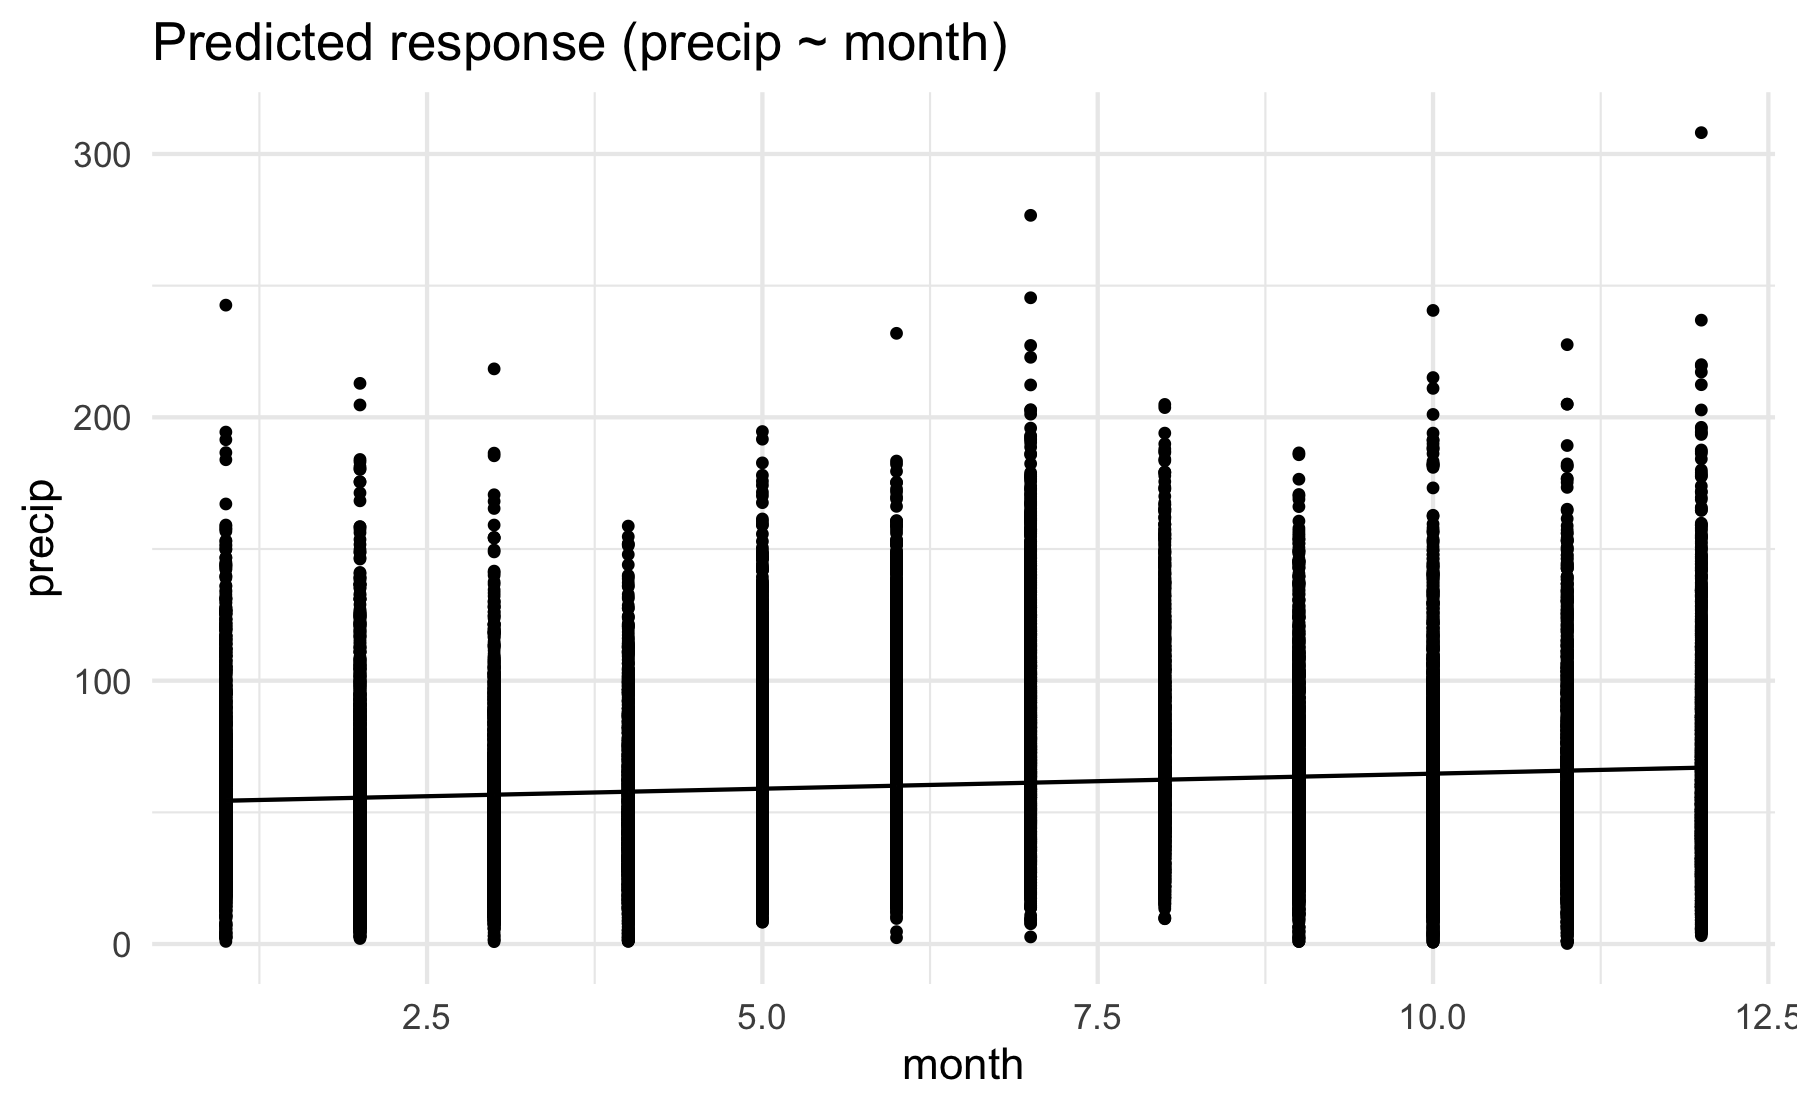
\includegraphics{img/fig-precip-month-num.png}

\subcaption{\label{}\texttt{lm\_wetter\_month}, Monat fälschlich als
metrische Variable}
\end{minipage}%
%
\begin{minipage}{0.50\linewidth}

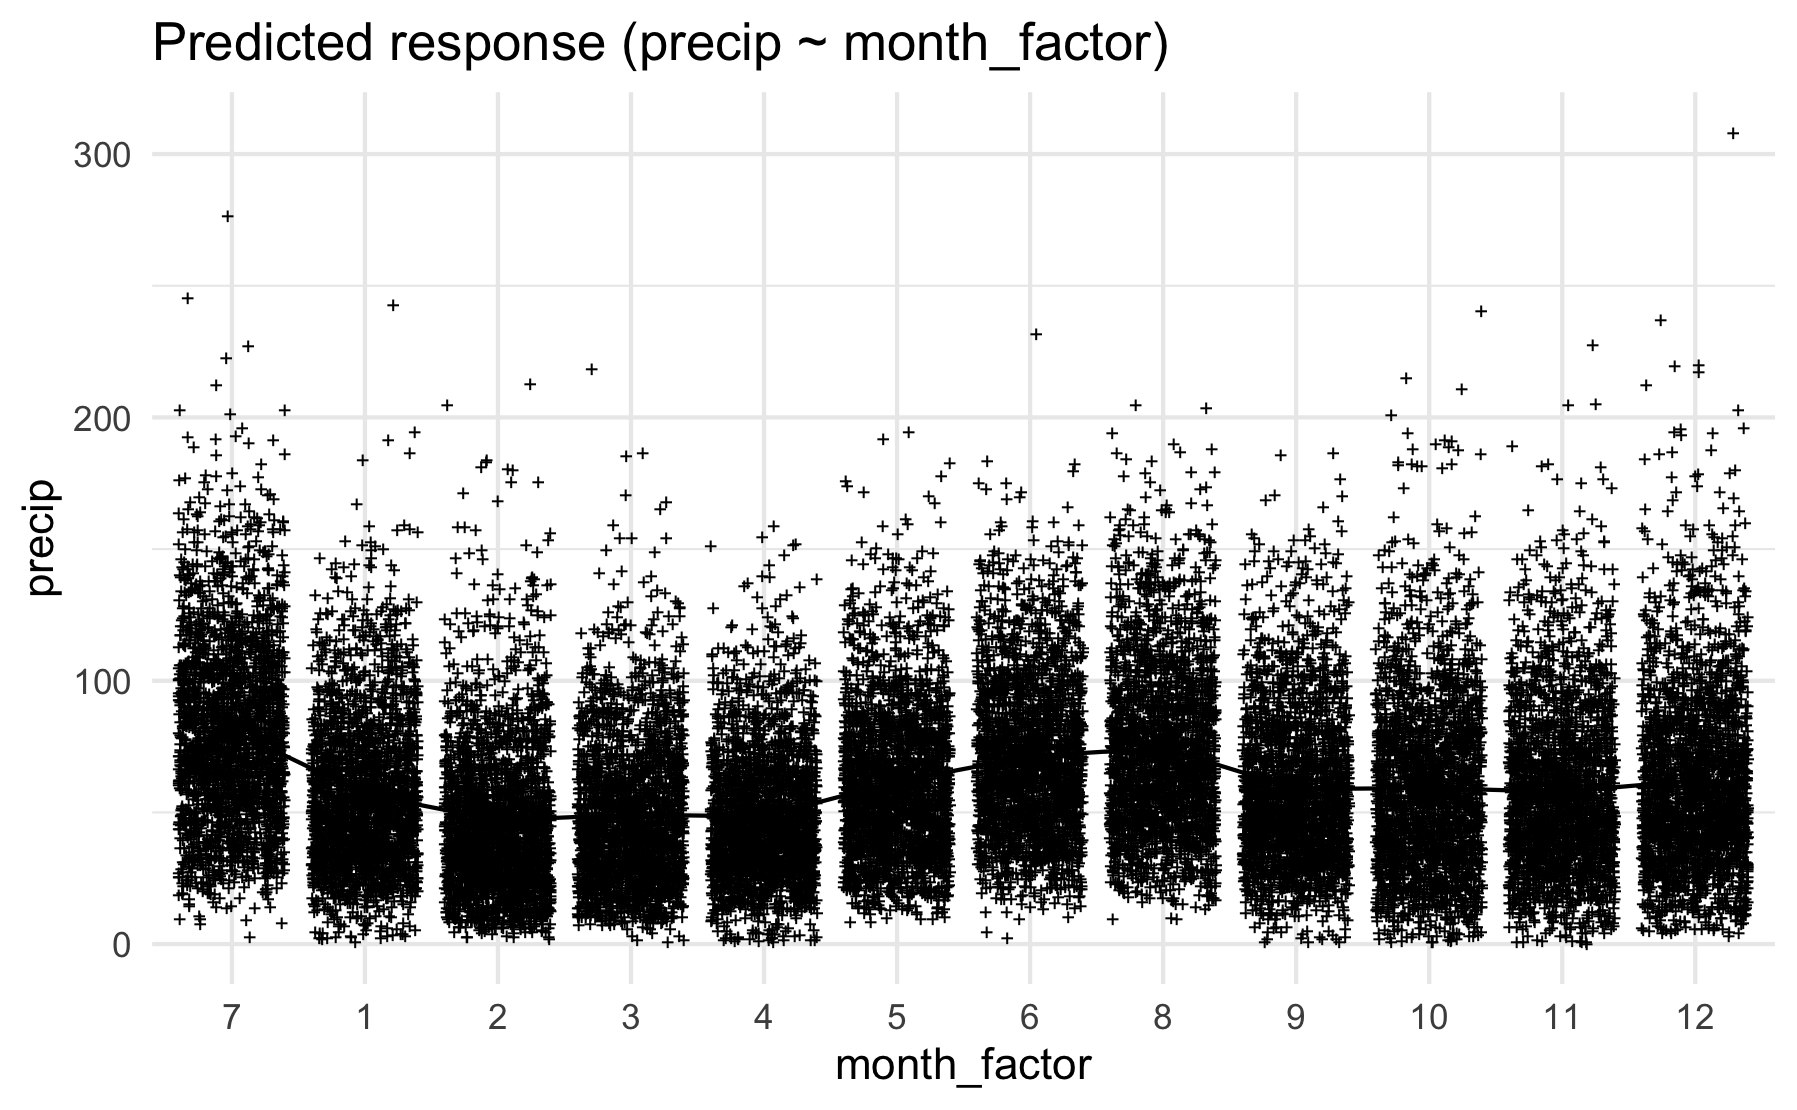
\includegraphics{img/fig-precip-month.png}

\subcaption{\label{}\texttt{lm\_wetter\_month\_text}, Monat korrekt als
nominale Variable (aber mit viel Overplotting, das müsste man besser
machen)}
\end{minipage}%

\caption{\label{fig-wetter-month}Niederschlagsunterschiede pro Monat
(ein Punkt ist ein Jahr); aufgrund der vielen Datenpunkte ist das
Diagramm wenig übersichtlich (Overplotting).}

\end{figure}%

Möchte man die Referenzgruppe eines Faktors ändern, kann man dies mit
\texttt{relevel} tun:

\begin{Shaded}
\begin{Highlighting}[]
\NormalTok{wetter }\OtherTok{\textless{}{-}}
\NormalTok{  wetter }\SpecialCharTok{\%\textgreater{}\%} 
  \FunctionTok{mutate}\NormalTok{(}\AttributeTok{month\_factor =} \FunctionTok{relevel}\NormalTok{(month\_factor, }\AttributeTok{ref =} \StringTok{"7"}\NormalTok{))}
\end{Highlighting}
\end{Shaded}

So sieht dann die geänderte Reihenfolge aus:\footnote{Zum
  Dollar-Operator s. \textbf{?@sec-dollar-op}}

\begin{Shaded}
\begin{Highlighting}[]
\FunctionTok{levels}\NormalTok{(wetter}\SpecialCharTok{$}\NormalTok{month\_factor)}
\DocumentationTok{\#\#  [1] "7"  "1"  "2"  "3"  "4"  "5"  "6"  "8"  "9"  "10" "11"}
\DocumentationTok{\#\# [12] "12"}
\end{Highlighting}
\end{Shaded}

\subsection{Binäre plus metrische UV}\label{sec-faktorvar}

In diesem Abschnitt untersuchen wir ein lineares Modell mit zwei UV:
einer \emph{zweistufigen} (binären) UV plus einer \emph{metrischen}
UV.\footnote{So ein Modell kann auch als \emph{Kovarianzanalyse} (engl.
  analysis of covariance, ancova) bezeichnet werden.}

\begin{example}[]\protect\hypertarget{exm-rain1}{}\label{exm-rain1}

Ob sich die Niederschlagsmenge wohl unterschiedlich zwischen den Monaten
entwickelt hat in den letzten gut 100 Jahren? Der Einfachheit halber
greifen Sie sich nur zwei Monate heraus (Januar und Juli).

\begin{Shaded}
\begin{Highlighting}[]
\NormalTok{wetter\_month\_1\_7 }\OtherTok{\textless{}{-}}
\NormalTok{  wetter }\SpecialCharTok{\%\textgreater{}\%} 
  \FunctionTok{filter}\NormalTok{(month }\SpecialCharTok{==} \DecValTok{1}  \SpecialCharTok{|}\NormalTok{ month }\SpecialCharTok{==} \DecValTok{7}\NormalTok{) }
\end{Highlighting}
\end{Shaded}

\begin{quote}
{\emoji{teacher}} Ich muss mal kurz auf eine Sache hinweisen\ldots{}
\end{quote}

\begin{tcolorbox}[enhanced jigsaw, bottomtitle=1mm, title=\textcolor{quarto-callout-note-color}{\faInfo}\hspace{0.5em}{Faktorvariable}, toptitle=1mm, arc=.35mm, bottomrule=.15mm, breakable, colbacktitle=quarto-callout-note-color!10!white, left=2mm, colframe=quarto-callout-note-color-frame, colback=white, opacityback=0, titlerule=0mm, rightrule=.15mm, opacitybacktitle=0.6, leftrule=.75mm, toprule=.15mm, coltitle=black]

Eine Faktorvariable ist einer der beiden Datentypen in R, die sich für
nominalskalierte Variablen anbieten: Textvariablen (\texttt{character})
und Faktor-Variablen (\texttt{factor}). Ein wichtiger Unterschied ist,
dass die erlaubten Ausprägungen (``Faktorstufen'') bei einer
Faktor-Variable mitgespeichert werden, bei der Text-Variable nicht.

Das kann praktisch sein, denn bei einer Faktorvariable ist immer klar,
welche Ausprägungen in Ihrer Variable möglich sind.\(\square\)

\end{tcolorbox}

\begin{example}[Beispiel für eine
Faktorvariable]\protect\hypertarget{exm-factor1}{}\label{exm-factor1}

~

\begin{Shaded}
\begin{Highlighting}[]
\NormalTok{geschlecht }\OtherTok{\textless{}{-}} \FunctionTok{c}\NormalTok{(}\StringTok{"f"}\NormalTok{, }\StringTok{"f"}\NormalTok{, }\StringTok{"m"}\NormalTok{)}
\NormalTok{geschlecht\_factor }\OtherTok{\textless{}{-}} \FunctionTok{factor}\NormalTok{(geschlecht)}
\NormalTok{geschlecht\_factor}
\DocumentationTok{\#\# [1] f f m}
\DocumentationTok{\#\# Levels: f m}
\end{Highlighting}
\end{Shaded}

\end{example}

\begin{example}[Filtern verändert die Faktorstufen
nicht]\protect\hypertarget{exm-factor2}{}\label{exm-factor2}

Wenn Sie von der Faktorvariablen\footnote{synonym: nominalskalierte
  Variable} \texttt{geschlecht} das 3. Element (\texttt{"m"})
herausfiltern, so dass z.B. nur die ersten beiden Elemente übrig bleiben
mit allein der Ausprägung \texttt{"f"}, merkt sich R trotzdem, dass es
\emph{zwei} Faktorstufen gibt (\texttt{"f"} und \texttt{"m"}).

Genaus so ist es, wenn Sie aus \texttt{wetter} nur die Monate
\texttt{"1"} und \texttt{"7"} herausfiltern: R merkt sich, dass es 12
Faktorstufen gibt. Möchten Sie die herausgefilterten Faktorstufen
``löschen'', so können Sie einfach die Faktorvariable neu berechnen (mit
\texttt{factor}).\(\square\)

\end{example}

\begin{Shaded}
\begin{Highlighting}[]
\NormalTok{wetter\_month\_1\_7 }\OtherTok{\textless{}{-}}
\NormalTok{  wetter }\SpecialCharTok{\%\textgreater{}\%} 
  \FunctionTok{filter}\NormalTok{(month }\SpecialCharTok{==} \DecValTok{1}  \SpecialCharTok{|}\NormalTok{ month }\SpecialCharTok{==} \DecValTok{7}\NormalTok{) }\SpecialCharTok{\%\textgreater{}\%} 
  \CommentTok{\# Faktor (und damit die Faktorstufen) neu berechnen:}
  \FunctionTok{mutate}\NormalTok{(}\AttributeTok{month\_factor =} \FunctionTok{factor}\NormalTok{(month))}
\end{Highlighting}
\end{Shaded}

Okay. Wie spezifiziert man jetzt das lineare Modell?\(\square\)

\end{example}

Hat man mehrere (``multiple'') X-Variablen\footnote{Prädiktoren,
  unabhängige Variablen, X-Variablen}, so trennt man sich mit einem
Plus-Zeichen in der Regressionsformel, z.B.
\texttt{temp\ \textasciitilde{}\ year\_c\ +\ month}.

\begin{tcolorbox}[enhanced jigsaw, bottomtitle=1mm, title=\textcolor{quarto-callout-important-color}{\faExclamation}\hspace{0.5em}{Multiple Regression}, toptitle=1mm, arc=.35mm, bottomrule=.15mm, breakable, colbacktitle=quarto-callout-important-color!10!white, left=2mm, colframe=quarto-callout-important-color-frame, colback=white, opacityback=0, titlerule=0mm, rightrule=.15mm, opacitybacktitle=0.6, leftrule=.75mm, toprule=.15mm, coltitle=black]

Eine multiple Regression beinhaltet mehr als eine X-Variable. Die
Modellformel spezifiziert man so:

\(y ~ x_1 + x_2 + \ldots + x_n \qquad \square\)

\end{tcolorbox}

\begin{tcolorbox}[enhanced jigsaw, bottomtitle=1mm, title=\textcolor{quarto-callout-note-color}{\faInfo}\hspace{0.5em}{Modellgleichung}, toptitle=1mm, arc=.35mm, bottomrule=.15mm, breakable, colbacktitle=quarto-callout-note-color!10!white, left=2mm, colframe=quarto-callout-note-color-frame, colback=white, opacityback=0, titlerule=0mm, rightrule=.15mm, opacitybacktitle=0.6, leftrule=.75mm, toprule=.15mm, coltitle=black]

Das Pluszeichen hat in der Modellgleichung\footnotemark{} \emph{keine}
arithmetische Funktion. Es wird nichts addiert. In der Modellgleichung
sagt das Pluszeichen nur ``und noch folgende UV\ldots{}''.\(\square\)

\end{tcolorbox}

\footnotetext{synonym: Regressionsformel}

Die obige Modellgleichung liest sich also so:

\begin{quote}
Temperatur ist eine Funktion von der (zentrierten) Jahreszahl und des
Monats
\end{quote}

\begin{Shaded}
\begin{Highlighting}[]
\NormalTok{lm\_year\_month }\OtherTok{\textless{}{-}} \FunctionTok{lm}\NormalTok{(precip }\SpecialCharTok{\textasciitilde{}}\NormalTok{ year\_c }\SpecialCharTok{+}\NormalTok{ month\_factor, }\AttributeTok{data =}\NormalTok{ wetter\_month\_1\_7)}
\end{Highlighting}
\end{Shaded}

Die Modellparameter sind in Tabelle~\ref{tbl-lm_year_month} zu sehen.

\begin{longtable}[]{@{}
  >{\raggedright\arraybackslash}p{(\columnwidth - 10\tabcolsep) * \real{0.2394}}
  >{\centering\arraybackslash}p{(\columnwidth - 10\tabcolsep) * \real{0.1831}}
  >{\centering\arraybackslash}p{(\columnwidth - 10\tabcolsep) * \real{0.0845}}
  >{\centering\arraybackslash}p{(\columnwidth - 10\tabcolsep) * \real{0.2535}}
  >{\centering\arraybackslash}p{(\columnwidth - 10\tabcolsep) * \real{0.1268}}
  >{\centering\arraybackslash}p{(\columnwidth - 10\tabcolsep) * \real{0.1127}}@{}}

\caption{\label{tbl-lm_year_month}Modellparameter von lm\_year\_month}

\tabularnewline

\toprule\noalign{}
\begin{minipage}[b]{\linewidth}\raggedright
Parameter
\end{minipage} & \begin{minipage}[b]{\linewidth}\centering
Coefficient
\end{minipage} & \begin{minipage}[b]{\linewidth}\centering
SE
\end{minipage} & \begin{minipage}[b]{\linewidth}\centering
95\% CI
\end{minipage} & \begin{minipage}[b]{\linewidth}\centering
t(4525)
\end{minipage} & \begin{minipage}[b]{\linewidth}\centering
p
\end{minipage} \\
\midrule\noalign{}
\endhead
\bottomrule\noalign{}
\endlastfoot
(Intercept) & 56.94 & 0.68 & (55.60, 58.27) & 83.57 & \textless{}
.001 \\
year c & 0.03 & 0.01 & (5.59e-03, 0.05) & 2.43 & 0.015 \\
month factor (7) & 24.37 & 0.97 & (22.48, 26.27) & 25.25 & \textless{}
.001 \\

\end{longtable}

Die Modellkoeffizienten sind so zu interpretieren:

\begin{enumerate}
\def\labelenumi{\arabic{enumi}.}
\tightlist
\item
  Achsenabschnitt (b0, \texttt{(Intercept})): Im Referenzjahr (1951) im
  \emph{Referenzmonat Januar} lag die Niederschlagsmenge bei 57 mm pro
  Quadratmeter.
\item
  Regressionskoeffizient für Jahr (b1, \texttt{year\_c}): Pro Jahr ist
  die Niederschlagsmenge im Schnitt um 0.02 mm an (im Referenzmonat).
\item
  Regressionskoeffizient für Monat (b2, \texttt{month\ {[}7{]}}) Im
  Monat \texttt{7} (Juli) lag die mittlere Niederschlagsmenge (im
  Referenzjahr) knapp 25 mm über dem mittleren Wert des Referenzmonats
  (Januar).
\end{enumerate}

Die Regressiongleichung von \texttt{lm\_year\_month} lautet:
\texttt{precip\_pred\ =\ 56.94\ +\ 0.03*year\_c\ +\ 24.37*month\_factor\_7}.

Im Monat Juli ist \texttt{month\_factor\_7\ =\ 1}, ansonsten (Januar)
ist \texttt{month\_factor\ =\ 0}.

\begin{quote}
{\emoji{student}} Puh, kompliziert!
\end{quote}

\begin{quote}
{\emoji{teacher}} Es gibt einen Trick, man kann sich von R einfach einen
beliebigen Y-Wert berechnen lassen, s. Beispiel~\ref{exm-niederschlag1}.
\end{quote}

\begin{example}[Niederschlag laut Modell Im Juli
2020?]\protect\hypertarget{exm-niederschlag1}{}\label{exm-niederschlag1}

Hey R, berechne uns anhand neuer Daten den laut Modell zu erwartenden
Niederschlag für Januar im Jahr 2020!

\begin{Shaded}
\begin{Highlighting}[]
\NormalTok{neue\_daten }\OtherTok{\textless{}{-}} \FunctionTok{tibble}\NormalTok{(}\AttributeTok{year\_c =} \DecValTok{2020{-}1951}\NormalTok{,}
                     \AttributeTok{month\_factor =} \FunctionTok{factor}\NormalTok{(}\StringTok{"1"}\NormalTok{))}
\FunctionTok{predict}\NormalTok{(lm\_year\_month, }\AttributeTok{newdata =}\NormalTok{ neue\_daten)}
\DocumentationTok{\#\#        1 }
\DocumentationTok{\#\# 58.92171}
\end{Highlighting}
\end{Shaded}

\end{example}

\begin{tcolorbox}[enhanced jigsaw, bottomtitle=1mm, title=\textcolor{quarto-callout-note-color}{\faInfo}\hspace{0.5em}{Hinweis}, toptitle=1mm, arc=.35mm, bottomrule=.15mm, breakable, colbacktitle=quarto-callout-note-color!10!white, left=2mm, colframe=quarto-callout-note-color-frame, colback=white, opacityback=0, titlerule=0mm, rightrule=.15mm, opacitybacktitle=0.6, leftrule=.75mm, toprule=.15mm, coltitle=black]

Alle Regressionskoeffizienten beziehen sich auf den Y-Wert \emph{unter
der Annahme, dass alle übrigen Prädiktoren den Wert Null (bzw.
Referenzwert) aufweisen}.\(\square\)

\end{tcolorbox}

Visualisieren wir uns die geschätzten Erwartungswert pro Prädiktorwert,
s. Abbildung~\ref{fig-lm3}:
\texttt{plot(estimate\_expectation(lm\_year\_month))}

\begin{figure}

\centering{

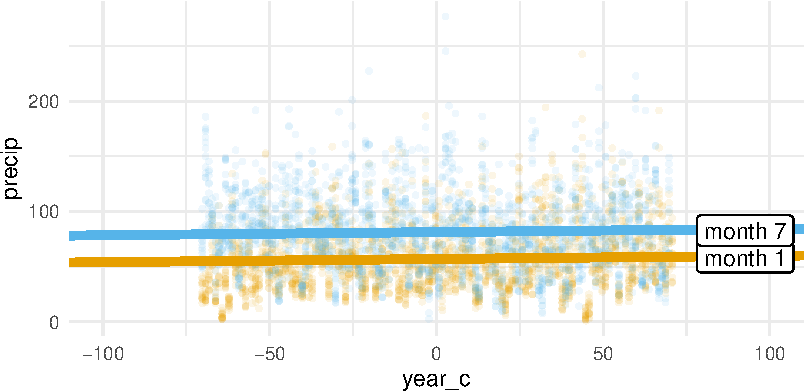
\includegraphics{090-regression2_files/figure-pdf/fig-lm3-1.pdf}

}

\caption{\label{fig-lm3}Temperaturverlauf über die Jahre für zwei
Monate. Man beachte, dass die Regressionsgeraden \emph{parallel} sind.}

\end{figure}%

Mit \texttt{scale\_color\_okabeito} haben wir die Standard-Farbpalette
durch die von (Okabe und Ito 2023) ersetzt\footnote{s. Hinweise hier:
  \url{https://malcolmbarrett.github.io/ggokabeito/reference/palette_okabe_ito.html}}.
Das ist nicht unbedingt nötig, aber robuster bei Schwarz-Weiß-Druck und
bei Sehschwächen, vgl. \textbf{?@sec-farbwahl}.

Die erklärte Varianz von \texttt{lm\_year\_month} liegt bei:

\begin{Shaded}
\begin{Highlighting}[]
\FunctionTok{r2}\NormalTok{(lm\_year\_month)}
\DocumentationTok{\#\# \# R2 for Linear Regression}
\DocumentationTok{\#\#        R2: 0.124}
\DocumentationTok{\#\#   adj. R2: 0.124}
\end{Highlighting}
\end{Shaded}

\subsection{Interaktion}\label{interaktion}

Eine Modellgleichung der Form
\texttt{temp\ \textasciitilde{}\ year\ +\ month} zwingt die
Regressionsgeraden dazu, parallel zu verlaufen. Aber vielleicht würden
sie besser in die Punktewolken passen, wenn wir ihnen erlauben, auch
\emph{nicht} parallel verlaufen zu dürfen?

Nicht-parallele Regressionsgeraden erlauben wir, indem wir das
Regressionsmodell wie folgt spezifizieren und visualisieren, s.
Listing~\ref{lst-lm-interact}.

\begin{codelisting}

\caption{\label{lst-lm-interact}Ein Interaktionsmodell spezifiziert man
in dieser Art: y \textasciitilde{} x1 + x2 + x1:x2}

\centering{

\begin{Shaded}
\begin{Highlighting}[]
\NormalTok{lm\_year\_month\_interaktion }\OtherTok{\textless{}{-}} \FunctionTok{lm}\NormalTok{(}
\NormalTok{  precip }\SpecialCharTok{\textasciitilde{}}\NormalTok{ year\_c }\SpecialCharTok{+}\NormalTok{ month\_factor }\SpecialCharTok{+}\NormalTok{ year\_c}\SpecialCharTok{:}\NormalTok{month\_factor, }
  \AttributeTok{data =}\NormalTok{ wetter\_month\_1\_7)}
\end{Highlighting}
\end{Shaded}

}

\end{codelisting}%

Visualisiert ist das Modell in Abbildung~\ref{fig-wetter-interakt}.

\begin{Shaded}
\begin{Highlighting}[]
\FunctionTok{plot}\NormalTok{(}\FunctionTok{estimate\_expectation}\NormalTok{(lm\_year\_month\_interaktion)) }\SpecialCharTok{+}
  \FunctionTok{scale\_color\_okabeito}\NormalTok{()  }\CommentTok{\# schönes Farbschema}
\end{Highlighting}
\end{Shaded}

\begin{figure}

\centering{

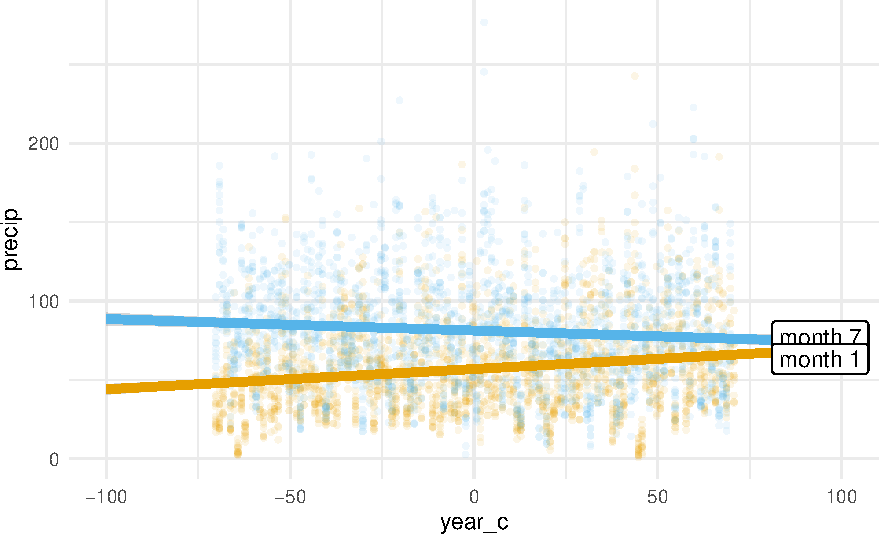
\includegraphics{090-regression2_files/figure-pdf/fig-wetter-interakt-1.pdf}

}

\caption{\label{fig-wetter-interakt}Niederschlag im Jahresverlauf und
Monatsvergleich mit Interaktionseffekt: Die Veränderung im Verlauf der
Jahre ist unterschiedlich für die Monate (Janur vs.~Juli). Die beiden
Regressionsgeraden sind \emph{nicht} parallel.}

\end{figure}%

Der \emph{Doppelpunkt-Operator} (\texttt{:}) fügt der
Regressionsgleichung einen \emph{Interaktionseffekt} hinzu, in diesem
Fall die Interaktion von Jahr (\texttt{year\_c}) und Monat
(\texttt{month\_factor}):

\texttt{precip\ \textasciitilde{}\ year\_c\ +\ month\_factor\ +\ year\_c:month\_factor}

\begin{tcolorbox}[enhanced jigsaw, bottomtitle=1mm, title=\textcolor{quarto-callout-important-color}{\faExclamation}\hspace{0.5em}{Wichtig}, toptitle=1mm, arc=.35mm, bottomrule=.15mm, breakable, colbacktitle=quarto-callout-important-color!10!white, left=2mm, colframe=quarto-callout-important-color-frame, colback=white, opacityback=0, titlerule=0mm, rightrule=.15mm, opacitybacktitle=0.6, leftrule=.75mm, toprule=.15mm, coltitle=black]

Einen Interaktionseffekt von x1 und x2 kennzeichnet man in R mit dem
Doppelpunkt-Operator, \texttt{x1:x2}:

\texttt{y\ \textasciitilde{}\ x1\ +\ x2\ +\ x1:x2} \(\square\)

\end{tcolorbox}

In Worten:

\begin{quote}
y wird modelliert als eine Funktion von x1 und x2 und dem
Interaktionseffekt von x1 mit x2.
\end{quote}

Wie man in Abbildung~\ref{fig-wetter-interakt} sieht, sind die beiden
Regressionsgeraden \emph{nicht parallel}.

\begin{tcolorbox}[enhanced jigsaw, bottomtitle=1mm, title=\textcolor{quarto-callout-note-color}{\faInfo}\hspace{0.5em}{Hinweis}, toptitle=1mm, arc=.35mm, bottomrule=.15mm, breakable, colbacktitle=quarto-callout-note-color!10!white, left=2mm, colframe=quarto-callout-note-color-frame, colback=white, opacityback=0, titlerule=0mm, rightrule=.15mm, opacitybacktitle=0.6, leftrule=.75mm, toprule=.15mm, coltitle=black]

Sind die Regressionsgeraden von zwei (oder mehr) Gruppen nicht parallel,
so liegt ein Interaktionseffekt vor.\(\square\)

\end{tcolorbox}

\begin{example}[Interaktionseffekt von Niederschlag und
Monat]\protect\hypertarget{exm-interakt-precip}{}\label{exm-interakt-precip}

Wie ist die Veränderung der Niederschlagsmenge (Y-Achse) im Verlauf der
Jahre (X-Achse)? \emph{Das kommt darauf an, welchen Monat man
betrachtet}. Der Effekt der Zeit ist \emph{unterschiedlich} für die
Monate: Im Juli nahm der Niederschlag ab, im Januar zu.\(\square\)

\end{example}

Liegt ein Interaktionseffekt vor, kann man nicht mehr von ``dem''
(statistischen) Effekt eines Prädiktors (afu die Y-Variable) sprechen.
Vielmehr muss man unterscheiden: Je nach Gruppe (z.B. Monat)
unterscheidet der Effekt.\footnote{Effekt ist hier immer statistisch,
  nie kausal gemeint.}

Betrachten wir die Parameterwerte des Interaktionsmodells
(\texttt{parameters(lm\_year\_month\_interaktion)}), s.
Tabelle~\ref{tbl-lm_year_month_interaktion}.

\begin{longtable}[]{@{}
  >{\raggedright\arraybackslash}p{(\columnwidth - 10\tabcolsep) * \real{0.3333}}
  >{\centering\arraybackslash}p{(\columnwidth - 10\tabcolsep) * \real{0.1667}}
  >{\centering\arraybackslash}p{(\columnwidth - 10\tabcolsep) * \real{0.0769}}
  >{\centering\arraybackslash}p{(\columnwidth - 10\tabcolsep) * \real{0.2051}}
  >{\centering\arraybackslash}p{(\columnwidth - 10\tabcolsep) * \real{0.1154}}
  >{\centering\arraybackslash}p{(\columnwidth - 10\tabcolsep) * \real{0.1026}}@{}}

\caption{\label{tbl-lm_year_month_interaktion}Modellparameter von
lm\_year\_month\_interaktion}

\tabularnewline

\toprule\noalign{}
\begin{minipage}[b]{\linewidth}\raggedright
Parameter
\end{minipage} & \begin{minipage}[b]{\linewidth}\centering
Coefficient
\end{minipage} & \begin{minipage}[b]{\linewidth}\centering
SE
\end{minipage} & \begin{minipage}[b]{\linewidth}\centering
95\% CI
\end{minipage} & \begin{minipage}[b]{\linewidth}\centering
t(4524)
\end{minipage} & \begin{minipage}[b]{\linewidth}\centering
p
\end{minipage} \\
\midrule\noalign{}
\endhead
\bottomrule\noalign{}
\endlastfoot
(Intercept) & 56.91 & 0.68 & (55.59, 58.24) & 84.21 & \textless{}
.001 \\
year c & 0.13 & 0.02 & (0.10, 0.16) & 7.80 & \textless{} .001 \\
month factor (7) & 24.37 & 0.96 & (22.50, 26.25) & 25.45 & \textless{}
.001 \\
year c × month factor (7) & -0.20 & 0.02 & (-0.25, -0.16) & -8.62 &
\textless{} .001 \\

\end{longtable}

Neu bei der Ausgabe zu diesem Modell ist die Zeile
\texttt{year\ c\ ×\ month\ factor\ {[}7{]}}. Sie gibt die Stärke des
Interaktionseffekts an. Die Zeile zeigt, wie unterschiedlich sich die
die Niederschlagsmenge zwischen den beiden Monaten im Verlauf der Jahre
ändert: Im Monat \texttt{"7"} ist der Effekt von \texttt{year\_c} um
0.20 mm geringer: Die Regressionsgerade neigt sich mehr nach ``unten''
im Monat Juli, da der Koeffizient kleiner als Null ist.

Die Regressionsgleichung lautet:
\texttt{precip\_pred\ =\ 56.91\ +\ 0.13*year\_c\ +\ 24.37*month\_factor\_7\ -\ 0.20*year\_c:month\_factor\_7}.

\begin{tcolorbox}[enhanced jigsaw, bottomtitle=1mm, title=\textcolor{quarto-callout-important-color}{\faExclamation}\hspace{0.5em}{Wichtig}, toptitle=1mm, arc=.35mm, bottomrule=.15mm, breakable, colbacktitle=quarto-callout-important-color!10!white, left=2mm, colframe=quarto-callout-important-color-frame, colback=white, opacityback=0, titlerule=0mm, rightrule=.15mm, opacitybacktitle=0.6, leftrule=.75mm, toprule=.15mm, coltitle=black]

Der Achsenabschnitt gibt den Wert für Y an unter der Annahme, dass alle
Prädiktoren den Wert Null aufweisen. In diesem Fall gibt der
Achsenabschnitt also den Niederschlag für den Janur des Jahres 1951 an.
Die Regressionskoeffizienten geben die Zunahme in Y an, wenn der
jeweilige Prädiktorwert um 1 steigt, die übrigen Prädiktoren aber den
Wert 0 aufweisen.\(\square\)

\end{tcolorbox}

Das R-Quadrat von \texttt{lm\_year\_month\_interaktion} beträgt übrigens
nur geringfügig mehr als im Modell ohne Interaktion:

\begin{Shaded}
\begin{Highlighting}[]
\FunctionTok{r2}\NormalTok{(lm\_year\_month\_interaktion)  }\CommentTok{\# aus \textasciigrave{}\{easystats\}\textasciigrave{}}
\DocumentationTok{\#\# \# R2 for Linear Regression}
\DocumentationTok{\#\#        R2: 0.139}
\DocumentationTok{\#\#   adj. R2: 0.138}
\end{Highlighting}
\end{Shaded}

\section{Modelle mit vielen UV}\label{modelle-mit-vielen-uv}

\subsection{Zwei metrische UV}\label{zwei-metrische-uv}

Ein Modell mit zwei metrischen UV kann man sich im 3D-Raum
visualisieren, s. Abbildung~\ref{fig-3d-regr-statisch}, oder im 2D-Raum,
s. Abbildung~\ref{fig-3d-regr-2d}. Im 3D-Raum wird die Regressionsgerade
zu einer \emph{Regressionsebene.}

\begin{figure}

\begin{minipage}{0.33\linewidth}

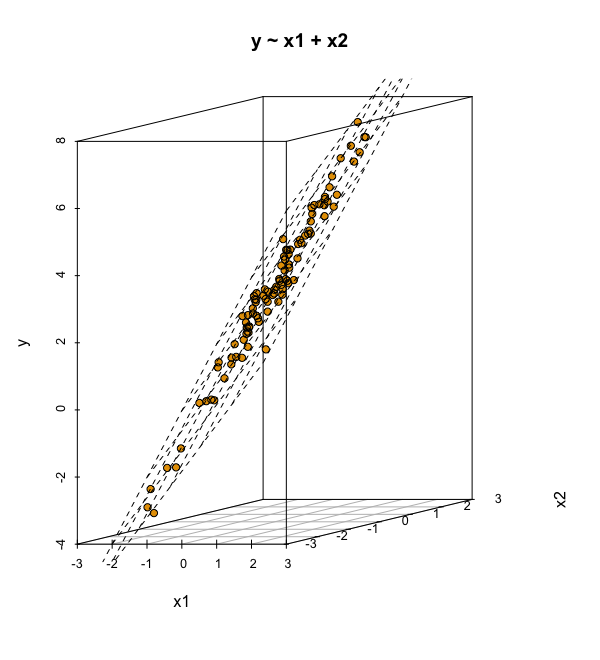
\includegraphics{img/3d_scatter1.png}

\subcaption{\label{}Winkel 1}
\end{minipage}%
%
\begin{minipage}{0.33\linewidth}

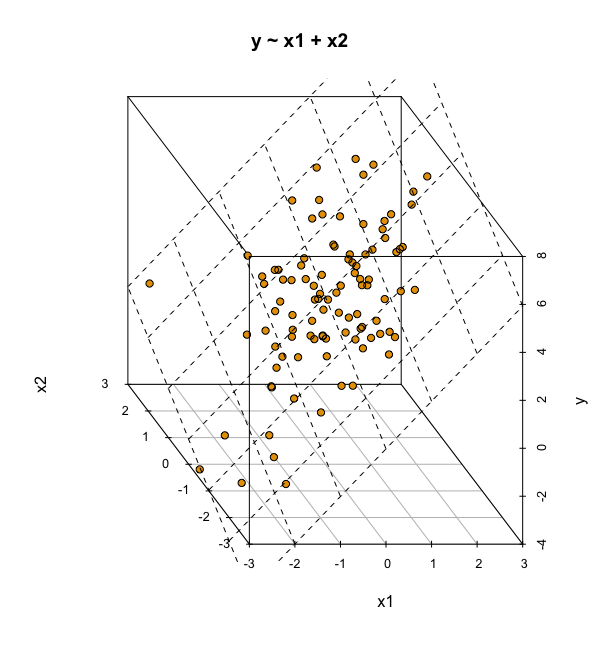
\includegraphics{img/3d_scatter2.png}

\subcaption{\label{}Winkel 2}
\end{minipage}%
%
\begin{minipage}{0.33\linewidth}

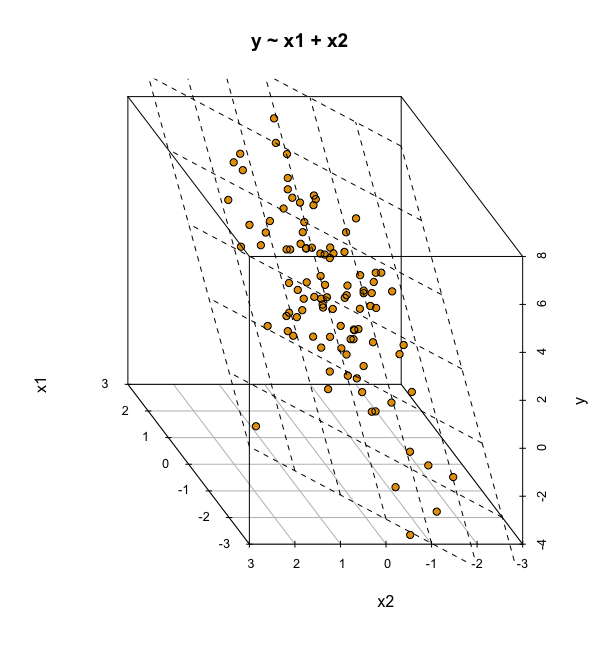
\includegraphics{img/3d_scatter3.png}

\subcaption{\label{}Winkel 3}
\end{minipage}%

\caption{\label{fig-3d-regr-statisch}Ein lineares Modell,
\texttt{y\ \textasciitilde{}\ x1\ +\ x2} mit zwei Prädiktoren im
3D-Raum.}

\end{figure}%

\begin{figure}

\centering{

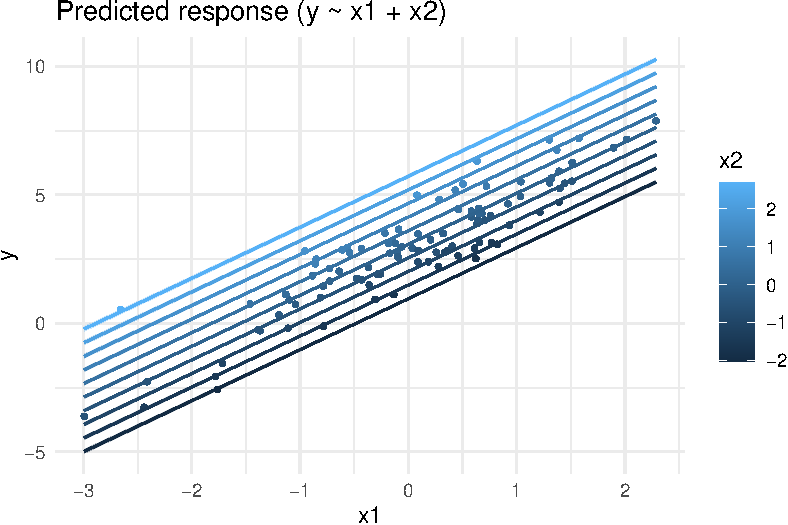
\includegraphics{090-regression2_files/figure-pdf/fig-3d-regr-2d-1.pdf}

}

\caption{\label{fig-3d-regr-2d}2D-Diagramm für 3D-Modell}

\end{figure}%

Grundsätzlich kann man viele Prädiktoren in ein (lineares) Modell
aufnehmen. Betrachten wir z. B. folgendes lineares Modell mit zwei
metrischen UV.

\begin{Shaded}
\begin{Highlighting}[]
\NormalTok{lm\_mario\_2uv }\OtherTok{\textless{}{-}} \FunctionTok{lm}\NormalTok{(total\_pr }\SpecialCharTok{\textasciitilde{}}\NormalTok{ start\_pr }\SpecialCharTok{+}\NormalTok{ ship\_pr, }\AttributeTok{data =}\NormalTok{ mariokart }\SpecialCharTok{\%\textgreater{}\%} \FunctionTok{filter}\NormalTok{(total\_pr }\SpecialCharTok{\textless{}} \DecValTok{100}\NormalTok{))}
\end{Highlighting}
\end{Shaded}

\textbf{?@fig-mario-2uv} visualisiert das Modell \texttt{lm\_mario2v} in
einem 3D-Diagramm (betrachtet aus verschiedenen Winkeln).

\begin{figure}

\begin{minipage}{0.33\linewidth}

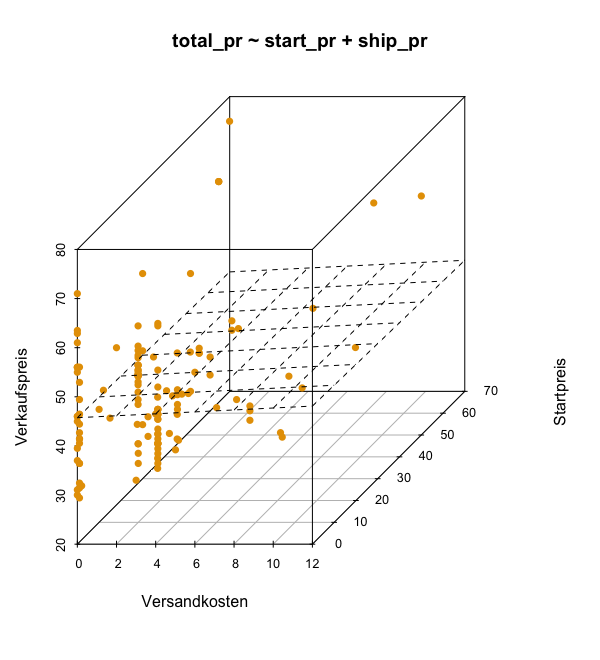
\includegraphics{img/3d_scatter_mario1.png}

\subcaption{\label{}Winkel 1}
\end{minipage}%
%
\begin{minipage}{0.33\linewidth}

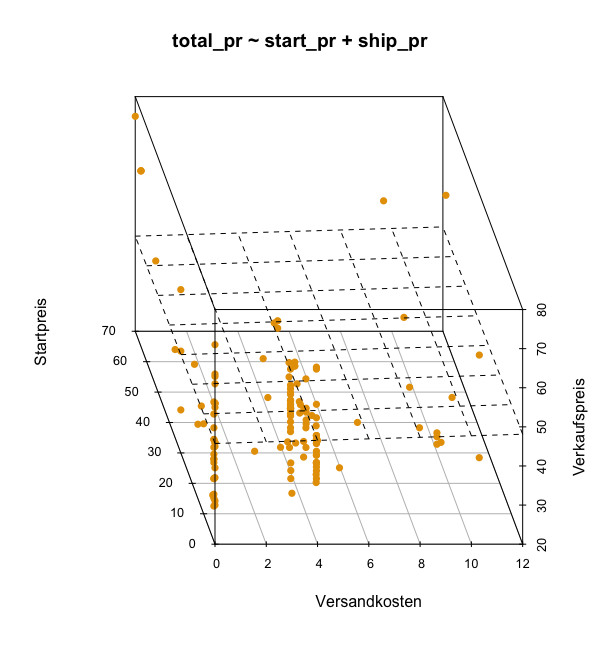
\includegraphics{img/3d_scatter_mario2.png}

\subcaption{\label{}Winkel 2}
\end{minipage}%
%
\begin{minipage}{0.33\linewidth}

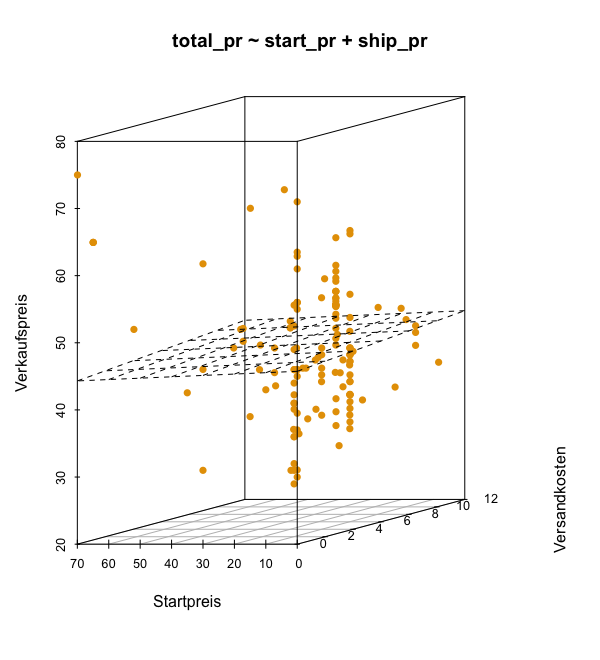
\includegraphics{img/3d_scatter_mario3.png}

\subcaption{\label{}Winkel 3}
\end{minipage}%

\caption{\label{fig-3d-regr-statisch}Das Modell \texttt{lm\_mario2v} mit
2 metrischen UV (und 1 metrische AV) als 3D-Diagramm}

\end{figure}%

\subsection{Viele UV ins Modell?}\label{viele-uv-ins-modell}

Wir könnten im Prinzip alle Variablen unserer Datentabelle als
Prädiktoren in das Regressionsmodell aufnehmen. Die Frage ist nur: Macht
das Sinn?

Hier sind einige Richtlinien, die helfen, welche Prädiktoren (und wie
viele) man in ein Modell aufnehmen sollte (Gelman, Hill, und Vehtari
2021), s. S. 199:

\begin{enumerate}
\def\labelenumi{\arabic{enumi}.}
\tightlist
\item
  Man sollte alle Prädiktoren aufnehmen, von denen anzunehmen ist, dass
  Sie Ursachen für die Zielvariablen sind
\item
  Bei Prädiktoren mit starken (absoluten) Effekten kann es Sinn machen,
  ihre Interaktionseffekte auch mit in das Modell aufzunehmen
\item
  Prädiktoren mit kleinem Schätzbereich (\texttt{95\ CI}) sollten
  tendenziell im Modell belassen werden, da sie die Modellgüte
  verbessern
\end{enumerate}

\section{Fallbeispiel zur Prognose}\label{fallbeispiel-zur-prognose}

\begin{example}[Prognose des
Verkaufspreis]\protect\hypertarget{exm-prognose}{}\label{exm-prognose}

Ganz können Sie von Business-Welt und ihren Gratifikationen nicht
lassen, trotz Ihrer wissenschaftlichen Ambitionen. Sie haben den Auftrag
bekommen, den Verkaufspreis von Mariokart-Spielen möglichst exakt
vorherzusagen. Also gut, das Honorar ist phantastisch, Sie sind jung und
brauchen das Geld.\(\square\)

\end{example}

\subsection{Modell ``all-in''}\label{modell-all-in}

Um die Güte Ihrer Vorhersagen zu prüfen, teilt Ihr Chef den Datensatz in
zwei zufällige Teile.

\begin{quote}
🧔‍♂️ Ich teile den Datensatz \texttt{mariokart} zufällig in zwei Teile.
Den ersten Teil kannst du nutzehn, um Modelle zu berechnen
(``trainieren'') und ihre Güte zu prüfen. Den Teil nenne ich
``Trainingssample'', hört sich cool an, oder? Im Train-Sample ist ein
Anteil (\texttt{frac}tion) von 70\% der Daten, okay? Die restlichen
Daten behalte ich. Wenn du ein gutes Modell hast, kommst du und wir
berechnen die Güte deiner Vorhersagen in dem verbleibenden Teil, die
übrigen 30\% der Daten. Diesen Teil nennen wir Test-Sample, alles klar?
\end{quote}

Wenn die Daten auf Ihrer Festplatte liegen, z.B. im Unterordner
\texttt{daten}, dann könne Sie sie von dort importieren:

\begin{Shaded}
\begin{Highlighting}[]
\NormalTok{mariokart\_train }\OtherTok{\textless{}{-}} \FunctionTok{read.csv}\NormalTok{(}\StringTok{"daten/mariokart\_train.csv"}\NormalTok{)}
\end{Highlighting}
\end{Shaded}

Alternativ können Sie sie auch von diesem Pfad von einem Rechner in der
Cloud herunterladen:

\begin{Shaded}
\begin{Highlighting}[]
\NormalTok{mariokart\_train\_path }\OtherTok{\textless{}{-}} \FunctionTok{paste0}\NormalTok{( }\StringTok{"https://raw.githubusercontent.com/sebastiansauer/"}\NormalTok{,}
\StringTok{"statistik1/main/daten/mariokart\_train.csv"}\NormalTok{)}

\NormalTok{mariokart\_train }\OtherTok{\textless{}{-}} \FunctionTok{read.csv}\NormalTok{(mariokart\_train\_path)}
\end{Highlighting}
\end{Shaded}

Dann importieren wir auf gleiche Weise Test-Sample in R:

\begin{Shaded}
\begin{Highlighting}[]
\NormalTok{mariokart\_test\_path }\OtherTok{\textless{}{-}} \FunctionTok{paste0}\NormalTok{(}
 \StringTok{"https://raw.githubusercontent.com/sebastiansauer/"}\NormalTok{,}
 \StringTok{"statistik1/main/daten/mariokart\_test.csv"}\NormalTok{)}

\NormalTok{mariokart\_test }\OtherTok{\textless{}{-}} \FunctionTok{read.csv}\NormalTok{(mariokart\_test\_path)}
\end{Highlighting}
\end{Shaded}

Also los. Sie probieren mal die ``All-in-Strategie'': Alle Variablen
rein in das Modell. Viel hilft viel, oder nicht?

\begin{Shaded}
\begin{Highlighting}[]
\NormalTok{lm\_allin }\OtherTok{\textless{}{-}} \FunctionTok{lm}\NormalTok{(total\_pr }\SpecialCharTok{\textasciitilde{}}\NormalTok{ ., }\AttributeTok{data =}\NormalTok{ mariokart\_train)}
\FunctionTok{r2}\NormalTok{(lm\_allin)  }\CommentTok{\# aus easystats}
\DocumentationTok{\#\# \# R2 for Linear Regression}
\DocumentationTok{\#\#        R2: 0.994}
\DocumentationTok{\#\#   adj. R2: 0.979}
\end{Highlighting}
\end{Shaded}

Der Punkt in \texttt{total\_pr\ \textasciitilde{}\ .} heißt ``alle
Variablen in der Tabelle (außer \texttt{total\_pr})''.

\begin{quote}
{\emoji{old-man}} Hey! Das ist ja fast perfekte Modellgüte!
\end{quote}

\begin{quote}
{\emoji{woman-supervillain}}️ Vorsicht: Wenn ein Angebot aussieht wie
``too good to be true'', dann ist es meist auch too good to be true.
\end{quote}

\begin{tcolorbox}[enhanced jigsaw, bottomtitle=1mm, title=\textcolor{quarto-callout-note-color}{\faInfo}\hspace{0.5em}{Overfitting}, toptitle=1mm, arc=.35mm, bottomrule=.15mm, breakable, colbacktitle=quarto-callout-note-color!10!white, left=2mm, colframe=quarto-callout-note-color-frame, colback=white, opacityback=0, titlerule=0mm, rightrule=.15mm, opacitybacktitle=0.6, leftrule=.75mm, toprule=.15mm, coltitle=black]

Der Grund für den fast perfekten Modellfit ist die Spalte
\texttt{Title}. Unser Modell hat einfach den Titel jeder Auktion
auswendig gelernt. Weiß man, welcher Titel zu welcher Auktion gehört,
kann man perfekt die Auktion aufsagen bzw. das Verkaufsgebot perfekt
vorhersagen. Leider nützen die Titel der Auktionen im Train-Sample
\emph{nichts} für andere Auktionen. Im Test-Sample werden unsere
Vorhersagen also grottenschlecht sein, wenn wir uns auf die Titel der
Auktionen im Test-Sample stützen. Merke: Höchst idiografische
Informationen wie Namen, Titel etc. sind nicht nützlich, um allgemeine
Muster zu erkennen und damit exakte Prognosen zu erstellen.\(\square\)

\end{tcolorbox}

Probieren wir also die Vorhersage im Test-Sample:

\begin{Shaded}
\begin{Highlighting}[]
\FunctionTok{predict}\NormalTok{(lm\_allin, }\AttributeTok{newdata =}\NormalTok{ mariokart\_test)}
\DocumentationTok{\#\# Error in eval(predvars, data, env): object \textquotesingle{}V1\textquotesingle{} not found}
\end{Highlighting}
\end{Shaded}

Oh nein! Was ist los!? Eine Fehlermeldung!

\begin{tcolorbox}[enhanced jigsaw, bottomtitle=1mm, title=\textcolor{quarto-callout-caution-color}{\faFire}\hspace{0.5em}{Vorsicht}, toptitle=1mm, arc=.35mm, bottomrule=.15mm, breakable, colbacktitle=quarto-callout-caution-color!10!white, left=2mm, colframe=quarto-callout-caution-color-frame, colback=white, opacityback=0, titlerule=0mm, rightrule=.15mm, opacitybacktitle=0.6, leftrule=.75mm, toprule=.15mm, coltitle=black]

Nominalskalierte Prädiktorvariablen mit vielen Ausprägungen, wie
\texttt{title} sind problematisch. Kommt eine Ausprägung von
\texttt{title} im Test-Sample vor, die es \emph{nicht} im Train-Sample
gab, so resultiert ein Fehler beim \texttt{predict}en. Häufig ist es
sinnvoll, auf diese Variable zu verzichten, da diese Variablen oft zu
Overfitting führen.\(\square\)

\end{tcolorbox}

\subsection{Modell ``all-in'', ohne
Titelspalte}\label{modell-all-in-ohne-titelspalte}

Okay, also auf die Titelspalte sollten wir vielleicht besser verzichten.
Nächster Versuch.

\begin{Shaded}
\begin{Highlighting}[]
\NormalTok{mariokart\_train2 }\OtherTok{\textless{}{-}}
\NormalTok{  mariokart\_train }\SpecialCharTok{\%\textgreater{}\%} 
  \FunctionTok{select}\NormalTok{(}\SpecialCharTok{{-}}\FunctionTok{c}\NormalTok{(title, V1, id))}
\end{Highlighting}
\end{Shaded}

Wir entfernen auch die Spalte \texttt{V1} und \texttt{id}, da sie
ebenfalls keine Informationen bergen.

\begin{Shaded}
\begin{Highlighting}[]
\NormalTok{lm\_allin\_no\_title }\OtherTok{\textless{}{-}} \FunctionTok{lm}\NormalTok{(total\_pr }\SpecialCharTok{\textasciitilde{}}\NormalTok{ ., }\AttributeTok{data =}\NormalTok{ mariokart\_train2)}
\FunctionTok{r2}\NormalTok{(lm\_allin\_no\_title) }
\DocumentationTok{\#\# \# R2 for Linear Regression}
\DocumentationTok{\#\#        R2: 0.521}
\DocumentationTok{\#\#   adj. R2: 0.441}
\end{Highlighting}
\end{Shaded}

Das R-Quadrat ist ja durchaus ordentlich. Schauen wir uns noch den
\texttt{rmse} (die SD der Vorhersagefehler) an\footnote{der Befehl wohnt
  im Paket \texttt{performance}, Teil des Metapakets \texttt{easystats}}:

\begin{quote}
{\emoji{robot}} Gut gemacht!
\end{quote}

\begin{Shaded}
\begin{Highlighting}[]
\NormalTok{performance}\SpecialCharTok{::}\FunctionTok{rmse}\NormalTok{(lm\_allin\_no\_title)}
\DocumentationTok{\#\# [1] 20.22998}
\end{Highlighting}
\end{Shaded}

\begin{tcolorbox}[enhanced jigsaw, bottomtitle=1mm, title=\textcolor{quarto-callout-caution-color}{\faFire}\hspace{0.5em}{Name Clash}, toptitle=1mm, arc=.35mm, bottomrule=.15mm, breakable, colbacktitle=quarto-callout-caution-color!10!white, left=2mm, colframe=quarto-callout-caution-color-frame, colback=white, opacityback=0, titlerule=0mm, rightrule=.15mm, opacitybacktitle=0.6, leftrule=.75mm, toprule=.15mm, coltitle=black]

Im Paket \texttt{yardstick} gibt es eine Funktion namens \texttt{rmse}
und im Paket \texttt{performance}, Teil des Meta-Pakets
\texttt{easystats} ebenfalls. Da sind Probleme vorprogrammiert. Das ist
so als würde die Lehrerin rufen: ``Schorsch, komm her!''. Dabei gibt es
zwei Schorsche in der Klasse: Den Müllers Schorsch und den Meiers
Schorsch. Sonst kommen beide, was die Lehrerin nicht will. Die Lehrerin
müsste also rufen: ``Müller Schorsch, komm her!''. Genau dasselbe machen
wir, wenn wir das R-Paket eines Befehls mitschreiben, sozusagen den
``Nachnamen'' des Befehls: \texttt{paketname::funktion} ist wie
\texttt{Müller::Schorsch}. In unserem Fall also:
\texttt{performance::rmse} Endlich weiß R wieder, was zu tun
ist!\(\square\)

\end{tcolorbox}

Sie rennen zu Ihrem Chef, der jetzt die Güte Ihrer Vorhersagen in den
\emph{restlichen} Daten bestimmen soll.

\begin{quote}
{\emoji{old-man}} Da wir dein Modell in diesem Teil des
Komplett-Datensatzes \emph{testen}, nennen wir diesen Teil das
``Test-Sample''.
\end{quote}

Ihr Chef schaut sich die Verkaufspreise im Test-Sample an:

\begin{Shaded}
\begin{Highlighting}[]
\NormalTok{mariokart\_test }\SpecialCharTok{\%\textgreater{}\%} 
  \FunctionTok{select}\NormalTok{(id, total\_pr) }\SpecialCharTok{\%\textgreater{}\%} 
  \FunctionTok{head}\NormalTok{()}
\end{Highlighting}
\end{Shaded}

\begin{longtable}[]{@{}rr@{}}
\toprule\noalign{}
id & total\_pr \\
\midrule\noalign{}
\endhead
\bottomrule\noalign{}
\endlastfoot
120477729093 & 37.02 \\
290355805215 & 54.99 \\
180415462166 & 56.01 \\
180415244903 & 56.00 \\
350261958546 & 64.95 \\
110443013258 & 46.50 \\
\end{longtable}

\begin{quote}
{\emoji{old-man}}️ Okay, hier sind die ersten paar echten Verkaufspreise.
Jetzt mach mal deine Vorhersagen auf Basis deines besten Modells!
\end{quote}

Hier sind Ihre Vorhersagen\footnote{engl. predictions; to predict:
  vorhersagen}:

\begin{Shaded}
\begin{Highlighting}[]
\NormalTok{lm\_allin\_predictions }\OtherTok{\textless{}{-}} \FunctionTok{predict}\NormalTok{(lm\_allin\_no\_title, }\AttributeTok{newdata =}\NormalTok{ mariokart\_test)}
\end{Highlighting}
\end{Shaded}

Hier sind Ihre ersten paar Vorhersagen:

\begin{Shaded}
\begin{Highlighting}[]
\FunctionTok{head}\NormalTok{(lm\_allin\_predictions)}
\DocumentationTok{\#\#        1        2        3        4        5        6 }
\DocumentationTok{\#\# 28.62826 53.85885 53.28035 54.03619 41.75512 46.57713}
\end{Highlighting}
\end{Shaded}

Dies Vorhersagen fügen wir noch der Ordnung halber in die Tabelle mit
den Test-Daten:

\begin{Shaded}
\begin{Highlighting}[]
\NormalTok{mariokart\_test }\OtherTok{\textless{}{-}}
\NormalTok{  mariokart\_test }\SpecialCharTok{\%\textgreater{}\%} 
  \FunctionTok{mutate}\NormalTok{(}\AttributeTok{lm\_allin\_predictions =} \FunctionTok{predict}\NormalTok{(lm\_allin\_no\_title, }\AttributeTok{newdata =}\NormalTok{ mariokart\_test))}
\end{Highlighting}
\end{Shaded}

Okay, was ist jetzt der mittlere Vorhersagefehler?

Um die Vorhersagegüte im Test-Sample auszurechnen\footnote{wir verwenden
  dazu die Funktionen \texttt{mae} und \texttt{rsq}}, nutzen wir die
Funktionen des R-Paketes \texttt{yardstick}\footnote{welches Sie
  vielleicht noch installieren müssen.}:

\begin{Shaded}
\begin{Highlighting}[]
\FunctionTok{library}\NormalTok{(yardstick)}

\NormalTok{yardstick}\SpecialCharTok{::}\FunctionTok{mae}\NormalTok{(}\AttributeTok{data =}\NormalTok{ mariokart\_test,}
               \AttributeTok{truth =}\NormalTok{ total\_pr,  }\CommentTok{\# echter Verkaufspreis}
               \AttributeTok{estimate =}\NormalTok{ lm\_allin\_predictions)  }\CommentTok{\# Ihre Vorhersage}
\NormalTok{yardstick}\SpecialCharTok{::}\FunctionTok{rmse}\NormalTok{(}\AttributeTok{data =}\NormalTok{ mariokart\_test,}
               \AttributeTok{truth =}\NormalTok{ total\_pr,  }\CommentTok{\# echter Verkaufspreis}
               \AttributeTok{estimate =}\NormalTok{ lm\_allin\_predictions)  }\CommentTok{\# Ihre Vorhersage}
\end{Highlighting}
\end{Shaded}

\begin{Shaded}
\begin{Highlighting}[]
\FunctionTok{library}\NormalTok{(yardstick)}

\NormalTok{yardstick}\SpecialCharTok{::}\FunctionTok{mae}\NormalTok{(}\AttributeTok{data =}\NormalTok{ mariokart\_test,}
               \AttributeTok{truth =}\NormalTok{ total\_pr,  }\CommentTok{\# echter Verkaufspreis}
               \AttributeTok{estimate =}\NormalTok{ lm\_allin\_predictions) }\SpecialCharTok{|\textgreater{}}  \CommentTok{\# Ihre Vorhersage}
\NormalTok{  knitr}\SpecialCharTok{::}\FunctionTok{kable}\NormalTok{()}
\NormalTok{yardstick}\SpecialCharTok{::}\FunctionTok{rmse}\NormalTok{(}\AttributeTok{data =}\NormalTok{ mariokart\_test,}
               \AttributeTok{truth =}\NormalTok{ total\_pr,  }\CommentTok{\# echter Verkaufspreis}
               \AttributeTok{estimate =}\NormalTok{ lm\_allin\_predictions)  }\SpecialCharTok{|\textgreater{}}  \CommentTok{\# Ihre Vorhersage}
\NormalTok{  knitr}\SpecialCharTok{::}\FunctionTok{kable}\NormalTok{()}
\end{Highlighting}
\end{Shaded}

Ihr mittlerer Vorhersagefehler (RMSE) liegt bei ca. 13 Euro.\footnote{Wir
  haben hier \texttt{yardstick::rmse} geschrieben und nicht nur
  \texttt{rmse}, da es sowohl im Paket \texttt{performance} ( Teil des
  Metapakets \texttt{easystats}) als auch im Paket \texttt{yardstick}
  (Teil des Metapakets \texttt{tidymodels}) einen Befehl des Namens
  \texttt{rmse\textasciigrave{}\textasciigrave{}\ gibt.\ Name-Clash-Alarm!\ \ R\ könnte\ daher\ den\ anderen}rmse``
  meinen als Sie, was garantiert zu Verwirrung führt. Entweder bei R
  oder bei Ihnen.}

\begin{quote}
{\emoji{old-man}} Ganz okay.
\end{quote}

Wie ist es um das R-Quadrat Ihrer Vorhersagen bestellt?

\begin{Shaded}
\begin{Highlighting}[]
\CommentTok{\# \textasciigrave{}rsq \textasciigrave{} ist auch aus dem Paket yardstick:}
\FunctionTok{rsq}\NormalTok{(}\AttributeTok{data =}\NormalTok{ mariokart\_test,}
    \AttributeTok{truth =}\NormalTok{ total\_pr,  }\CommentTok{\# echter Verkaufspreis}
    \AttributeTok{estimate =}\NormalTok{ lm\_allin\_predictions)  }\CommentTok{\# Ihre Vorhersage}
\end{Highlighting}
\end{Shaded}

\begin{longtable}[]{@{}llr@{}}
\toprule\noalign{}
.metric & .estimator & .estimate \\
\midrule\noalign{}
\endhead
\bottomrule\noalign{}
\endlastfoot
rsq & standard & 0.1741705 \\
\end{longtable}

\begin{quote}
{\emoji{old-man}}️ 17\%, nicht berauschend, aber immerhin!
\end{quote}

\begin{tcolorbox}[enhanced jigsaw, bottomtitle=1mm, title=\textcolor{quarto-callout-note-color}{\faInfo}\hspace{0.5em}{Modellgüte im Test-Sample meist geringer als im Train-Sample}, toptitle=1mm, arc=.35mm, bottomrule=.15mm, breakable, colbacktitle=quarto-callout-note-color!10!white, left=2mm, colframe=quarto-callout-note-color-frame, colback=white, opacityback=0, titlerule=0mm, rightrule=.15mm, opacitybacktitle=0.6, leftrule=.75mm, toprule=.15mm, coltitle=black]

Wie das Beispiel zeigt, ist die Modellgüte im Test-Sample (leider) oft
\emph{geringer} als im Train-Sample. Die Modellgüte im Train-Sample ist
mitunter übermäßig optimistisch. Dieses Phänomen bezeichnet man als
\emph{Overfitting}.\(\square\)

\end{tcolorbox}

\begin{tcolorbox}[enhanced jigsaw, bottomtitle=1mm, title=\textcolor{quarto-callout-tip-color}{\faLightbulb}\hspace{0.5em}{Tipp}, toptitle=1mm, arc=.35mm, bottomrule=.15mm, breakable, colbacktitle=quarto-callout-tip-color!10!white, left=2mm, colframe=quarto-callout-tip-color-frame, colback=white, opacityback=0, titlerule=0mm, rightrule=.15mm, opacitybacktitle=0.6, leftrule=.75mm, toprule=.15mm, coltitle=black]

Bevor man Vorhersagen eines Modells einreicht, bietet es sich, die
Modellgüte in einem neuen Datensatz, als einem Test-Sample, zu
überprüfen.\(\square\)

\end{tcolorbox}

\section{Vertiefung: Das Aufteilen Ihrer
Daten}\label{vertiefung-das-aufteilen-ihrer-daten}

\subsection{Analyse- und
Assessment-Sample}\label{analyse--und-assessment-sample}

Wenn Sie eine robuste Schätzung der Güte Ihres Modells erfahren möchten,
bietet sich folgendes Vorgehen an (vgl.
Abbildung~\ref{fig-sample-types}):

\begin{enumerate}
\def\labelenumi{\arabic{enumi}.}
\tightlist
\item
  Teilen Sie Ihren Datensatz (das Train-Sample) in zwei Teile: Das sog.
  Validation-Sample und das sog. Assessment-Sample.
\item
  Berechnen Sie Ihr Modell im ersten Teil Ihres Datensatzes (dem
  \emph{Validation-Sample}).
\item
  Prüfen Sie die Modellgüte im zweiten Teil Ihres Datensatzes (dem
  \emph{Assessment-Sample})
\end{enumerate}

Diese Aufteilung Ihres Datensatzatzes in diese zwei Teile nennt man auch
\emph{Validierungsaufteilung} (validation split); Sie können sie z.B. so
bewerkstelligen:

\begin{Shaded}
\begin{Highlighting}[]
\FunctionTok{library}\NormalTok{(rsample)}
\NormalTok{mariokart }\OtherTok{\textless{}{-}} \FunctionTok{read\_csv}\NormalTok{(}\StringTok{"daten/mariokart.csv"}\NormalTok{)  }\CommentTok{\# Wenn die CSV{-}Datei in einem Unterordner mit Namen "daten" liegt}

\NormalTok{meine\_aufteilung }\OtherTok{\textless{}{-}} \FunctionTok{initial\_split}\NormalTok{(mariokart, }\AttributeTok{strata =}\NormalTok{ total\_pr)}
\end{Highlighting}
\end{Shaded}

\texttt{initial\_split} \emph{bestimmt} für jede Zeile (Beobachtung)
zufällig aus, ob diese Zeile in das Analyse- oder in das
Assessment-Sample kommen soll. Im Standard werden 75\% der Daten in das
Analyse- und 25\% in das Assessment-Sample eingeteilt\footnote{vgl.
  \texttt{help(initial\_split)}}; das ist eine sinnvolle Aufteilung. Das
Argument \texttt{strata} sorgt dafür, dass die Verteilung der AV in
beiden Stichproben gleich ist. Es wäre nämlich blöd für Ihr Modell, wenn
im Train-Sample z.B. nur die teuren, und im Test-Sample nur die
günstigen Spiele landen würde.\footnote{Anderes Beispiel: In den ersten
  Zeilen stehen nur Kunden aus Land A und in den unteren Zeilen nur aus
  Land B.} In so einem Fall würde sich Ihr Modell unnötig schwer tun.

Im nächsten Schritt können Sie anhand anhand der von
\texttt{initial\_split} bestimmten Aufteilung die Daten tatsächlich
aufteilen.\footnote{initial\_split sagt nur, welche Zeile in welche der
  beiden Stichproben kommen \emph{soll}. Die eigentliche Aufteilung wird
  aber noch nicht durchgeführt.}

\begin{Shaded}
\begin{Highlighting}[]
\NormalTok{mariokart\_train }\OtherTok{\textless{}{-}} \FunctionTok{training}\NormalTok{(meine\_aufteilung)  }\CommentTok{\# Analyse{-}Sample}
\NormalTok{mariokart\_test }\OtherTok{\textless{}{-}} \FunctionTok{testing}\NormalTok{(meine\_aufteilung)  }\CommentTok{\# Assessment{-}Sample}
\end{Highlighting}
\end{Shaded}

Ich persönliche nenne die Tabelle mit den Daten gerne
\texttt{d\_analysis} bzw. \texttt{d\_assess}, das ist kürzer zu tippen
und einheitlich. Sie können aber auch ein eigenes Namens-Schema nutzen;
was aber hilfreich ist, ist Konsistenz in der Benamung, außerdem Kürze
und aussagekräftige Namen.

\subsection{Train- vs.~Test-Sample}\label{train--vs.-test-sample}

\begin{definition}[Train-Sample]\protect\hypertarget{def-trainsample}{}\label{def-trainsample}

Den Datensatz, für die Sie sowohl UV \emph{als auch AV} vorliegen haben,
nennt man Train-Sample. \(\square\)

\end{definition}

Das Train-Sample stellt die bekannten Daten dar; aus denen können wir
lernen, d.h. unser Modell berechnen.

\begin{definition}[Test-Sample]\protect\hypertarget{def-testsample}{}\label{def-testsample}

Den Datensatz, für den Sie \emph{nur} Daten der UV, aber nicht zu der AV
vorliegen haben, nennt man \emph{Test-Sample}. \(\square\)

\end{definition}

Das Test-Sample stellt das Problem der wirklichen Welt dar: Neue
Beobachtungen, von denen man (noch) nicht weiß, was der Wert der AV ist.

Der Zusammenhang dieser verschiedenen, aber zusammengehörigen Arten von
Stichproben ist in Abbildung~\ref{fig-sample-types} dargestellt.

\begin{figure}

\centering{

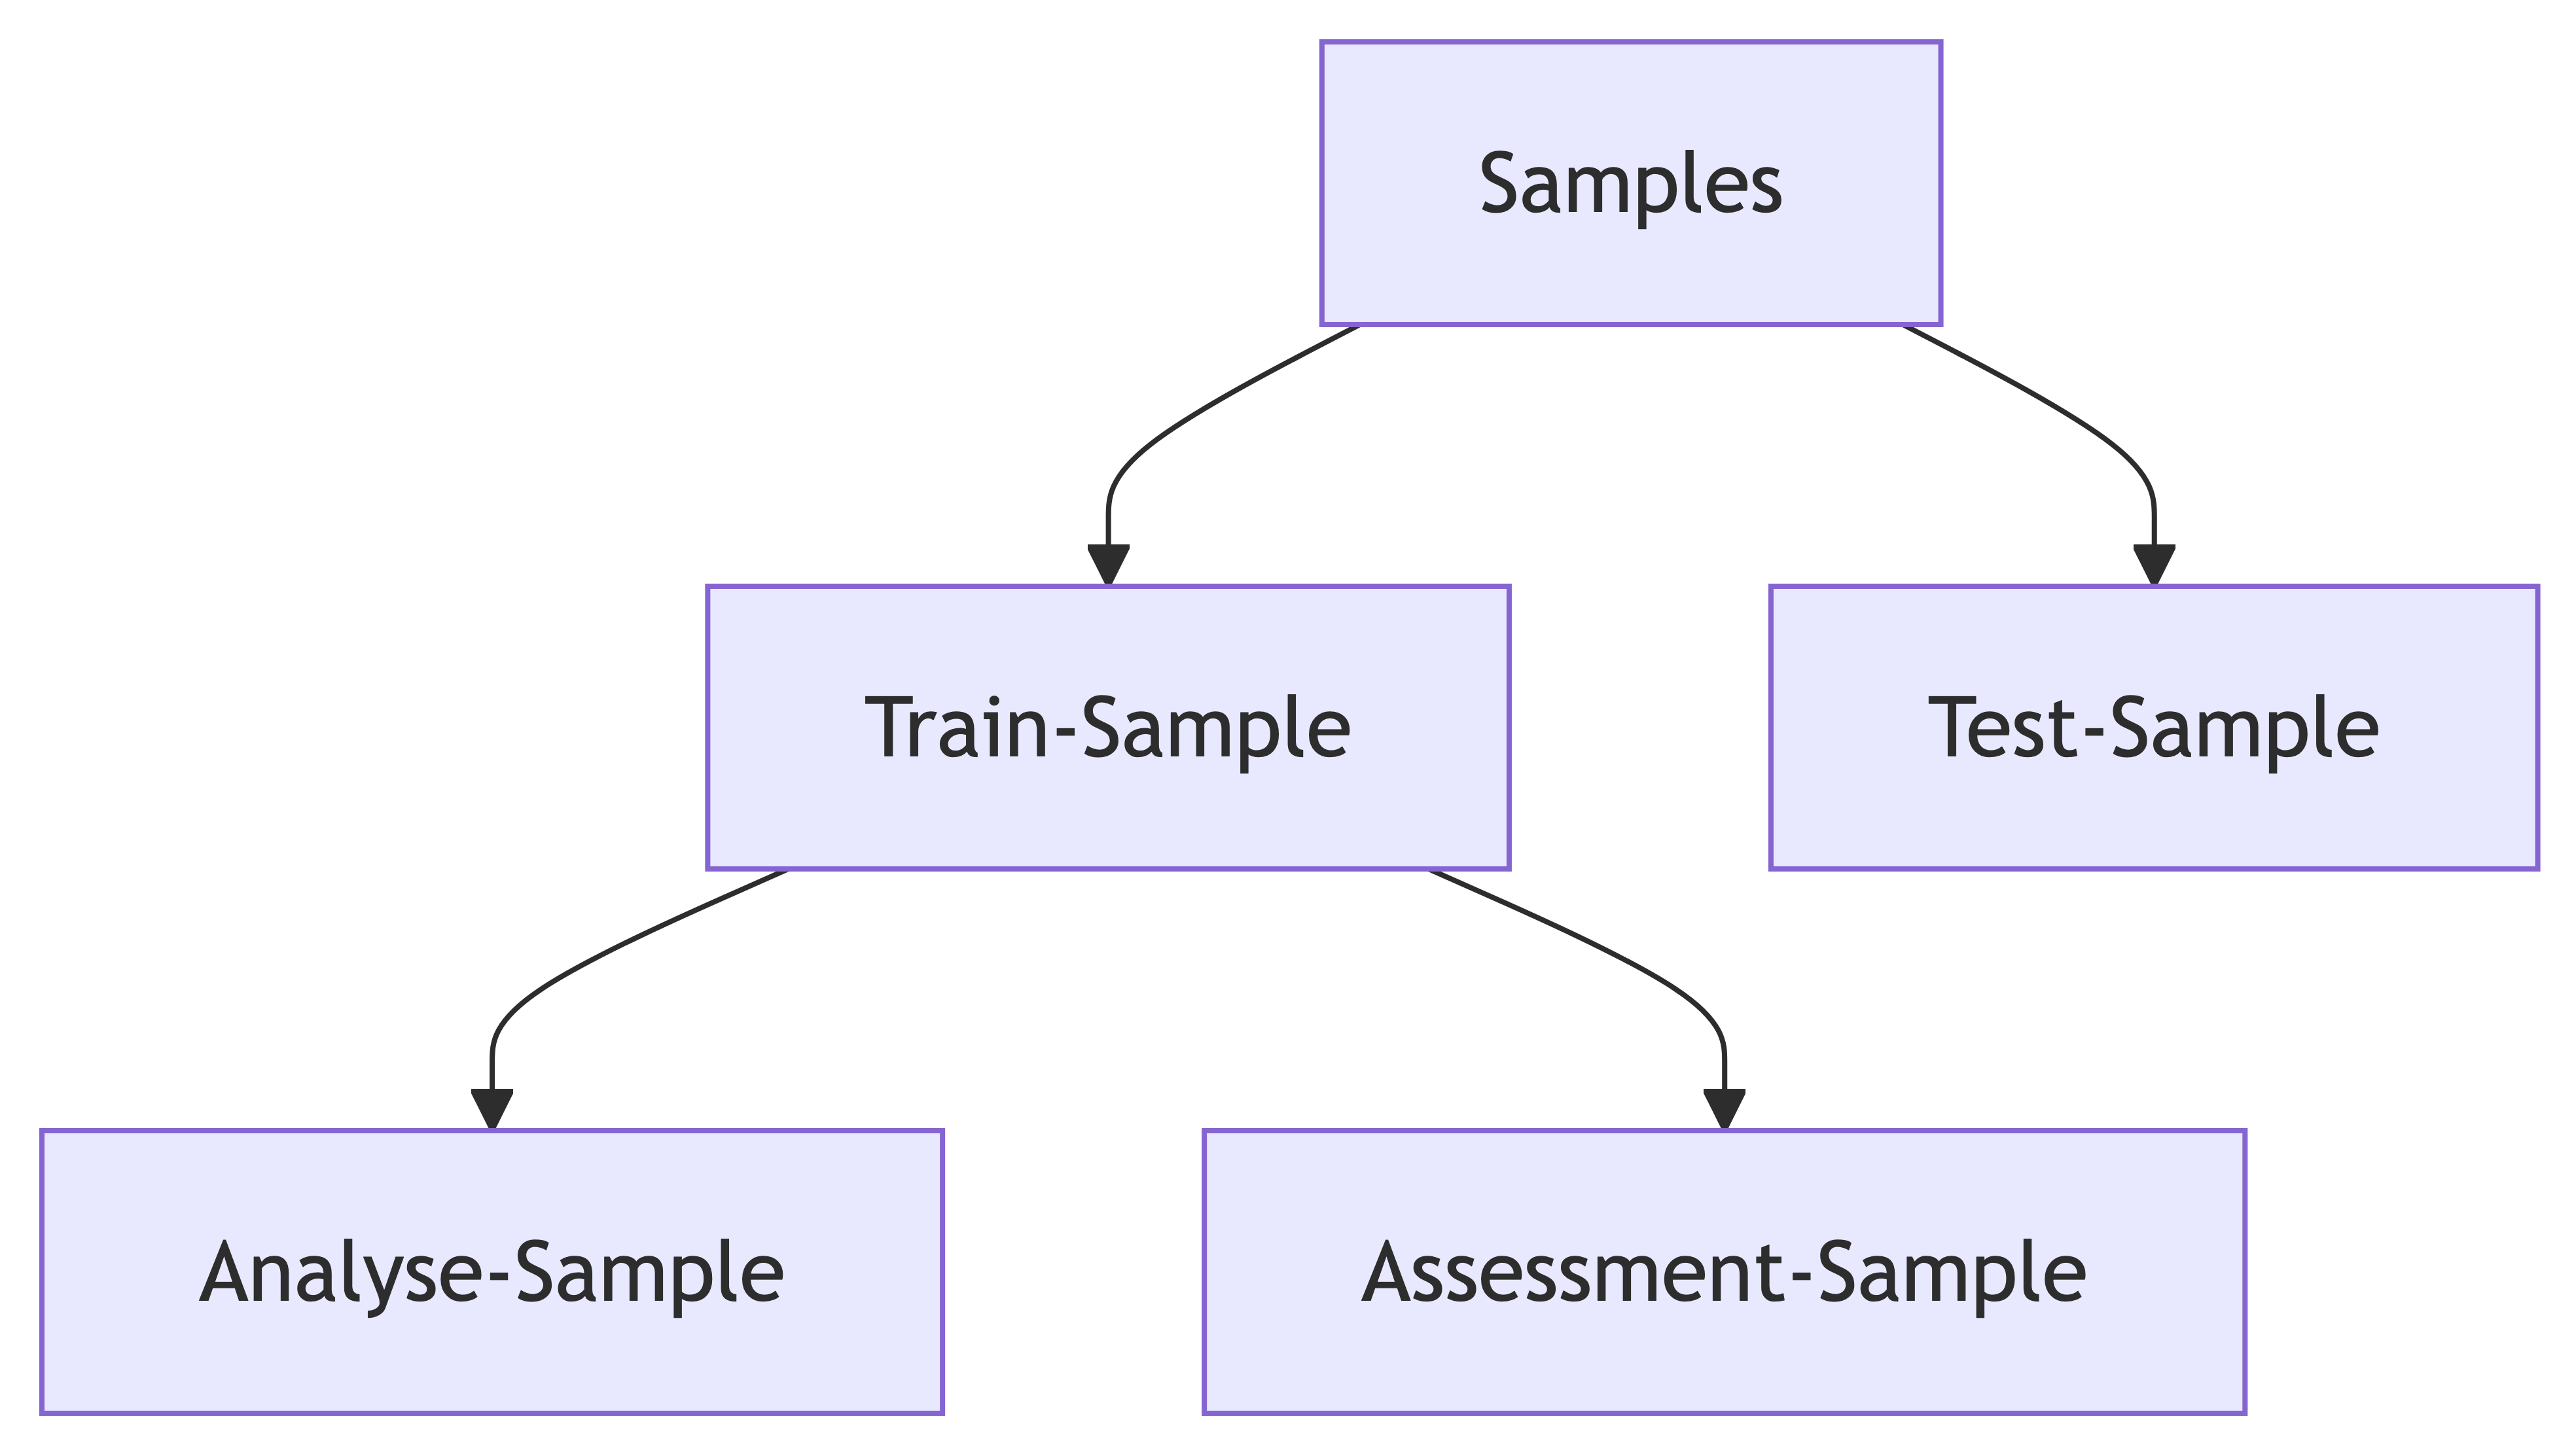
\includegraphics[width=3.96in,height=2.26in]{090-regression2_files/figure-latex/mermaid-figure-1.png}

}

\caption{\label{fig-sample-types}Verschiedene Arten von
zusammengehörigen Stichprobenarten im Rahmen einer Prognosemodellierung}

\end{figure}%

\section{Praxisbezug}\label{praxisbezug}

Ein Anwendungsbezug von moderner Datenanalyse ist es vorherzusagen,
welche Kunden ``abwanderungsgefährdet'' sind, also vielleicht in Zukunft
bald nicht mehr unsere Kunden sind (``customer churn''). Es gibt eine
ganze Reihe von Untersuchungen dazu, z.B. die von
(\textbf{lalwani\_customer\_2022?}). Die Forschis versuchen anhand von
Daten und u.a. auch der linearen Regression vorherzusagen, welche Kunden
abgewandert sein werden. Die Autoren berichten von einer Genauigkeit von
über 80\% in Ihrem (besten) Vorhersagemodell.

\section{Wie man mit Statistik
lügt}\label{wie-man-mit-statistik-luxfcgt}

\subsection{Pinguine drehen durch}\label{pinguine-drehen-durch}

Ein Forscher-Team untersucht Pinguine von der
\href{https://pallter.marine.rutgers.edu/}{Palmer Station, Antarktis}.
Das Team ist am Zusammenhang von Schnabellänge (\emph{bill length}) und
Schnabeltiefe (\emph{bill depth}) interessiert, s.
Abbildung~\ref{fig-peng-bill}.

\begin{figure}

\centering{

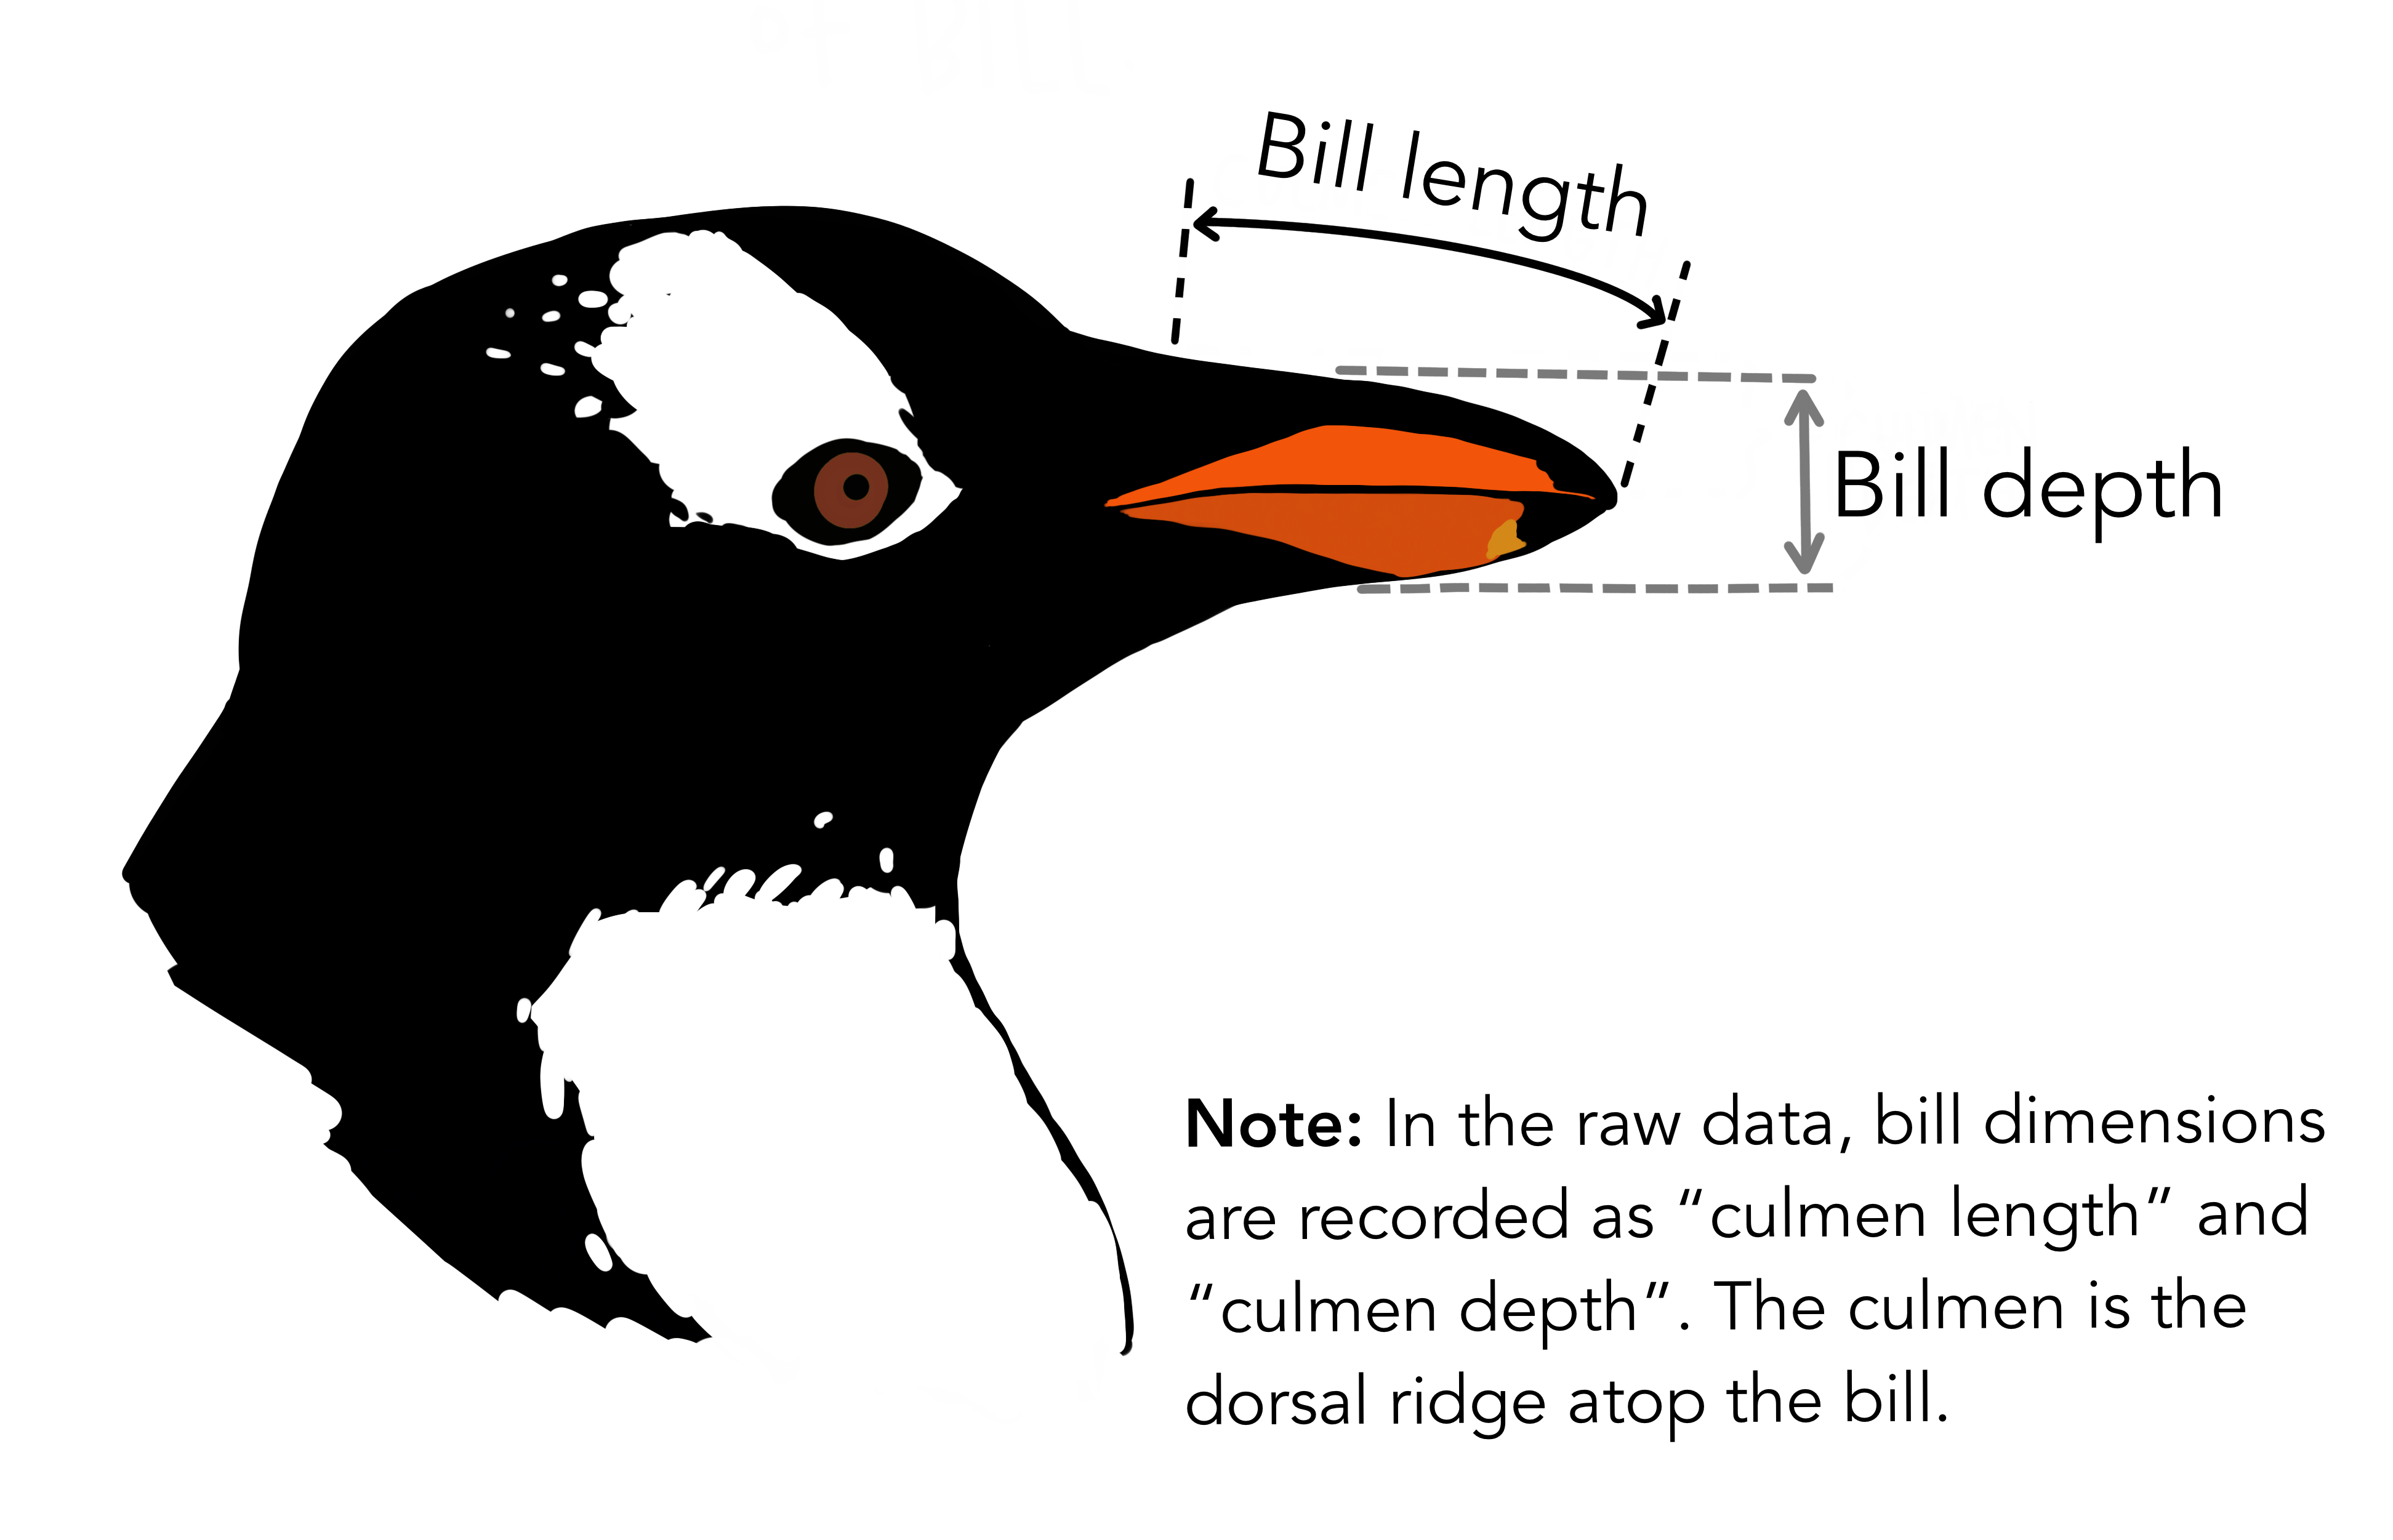
\includegraphics[width=0.5\textwidth,height=\textheight]{index_files/mediabag/culmen_depth.png}

}

\caption{\label{fig-peng-bill}Schnabellänge und Schnabeltiefe}

\end{figure}%

Das Team hat in \st{schweißtreibender} eiszapfentreibender Arbeit
\(n=344\) Tiere vermessen bei antarktischen Temperaturen. Hier sind die
Daten:

\begin{Shaded}
\begin{Highlighting}[]
\NormalTok{penguins\_path }\OtherTok{\textless{}{-}} \FunctionTok{paste0}\NormalTok{(}
  \StringTok{"https://vincentarelbundock.github.io/"}\NormalTok{,}
  \StringTok{"Rdatasets/csv/palmerpenguins/penguins.csv"}\NormalTok{)}

\NormalTok{penguins }\OtherTok{\textless{}{-}} \FunctionTok{read.csv}\NormalTok{(penguins\_path)}
\end{Highlighting}
\end{Shaded}

\subsection{Analyse 1: Gesamtdaten}\label{analyse-1-gesamtdaten}

Man untersucht, rechnet und überlegt. Ah! Jetzt haben wir es! Klarer
Fall: Ein \emph{negativer} Zusammenhang von Schnabellänge und
Schnabeltiefe. Das könnte einen Nobelpreis wert sein. Schnell
publizieren!

\begin{Shaded}
\begin{Highlighting}[]
\FunctionTok{ggscatter}\NormalTok{(penguins, }\AttributeTok{x =} \StringTok{"bill\_length\_mm"}\NormalTok{, }\AttributeTok{y =} \StringTok{"bill\_depth\_mm"}\NormalTok{, }
          \AttributeTok{add =} \StringTok{"reg.line"}\NormalTok{)  }\CommentTok{\# aus \textasciigrave{}ggpubr\textasciigrave{}}
\end{Highlighting}
\end{Shaded}

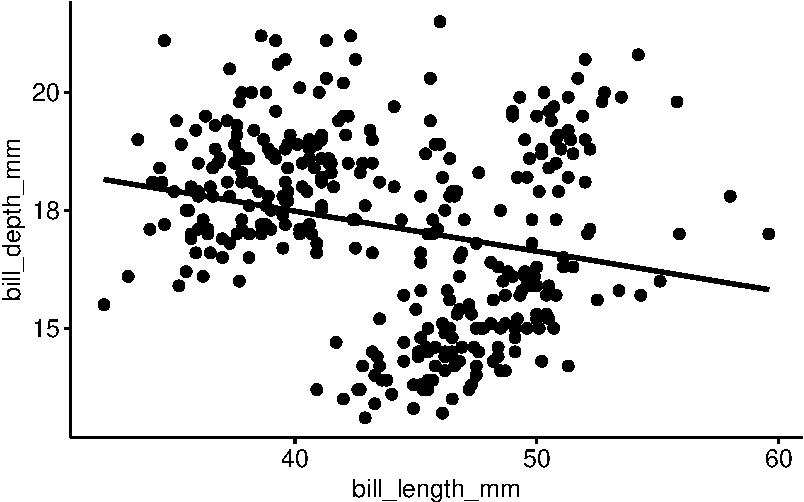
\includegraphics{090-regression2_files/figure-pdf/unnamed-chunk-62-1.pdf}

Hier sind die statistischen Details, s. Tabelle~\ref{tbl-peng-simpson1}.

\begin{Shaded}
\begin{Highlighting}[]
\NormalTok{lm1 }\OtherTok{\textless{}{-}} \FunctionTok{lm}\NormalTok{(bill\_depth\_mm }\SpecialCharTok{\textasciitilde{}}\NormalTok{ bill\_length\_mm, }\AttributeTok{data =}\NormalTok{ penguins)}
\end{Highlighting}
\end{Shaded}

\begin{longtable}[]{@{}
  >{\raggedright\arraybackslash}p{(\columnwidth - 10\tabcolsep) * \real{0.2273}}
  >{\centering\arraybackslash}p{(\columnwidth - 10\tabcolsep) * \real{0.1970}}
  >{\centering\arraybackslash}p{(\columnwidth - 10\tabcolsep) * \real{0.0909}}
  >{\centering\arraybackslash}p{(\columnwidth - 10\tabcolsep) * \real{0.2424}}
  >{\centering\arraybackslash}p{(\columnwidth - 10\tabcolsep) * \real{0.1212}}
  >{\centering\arraybackslash}p{(\columnwidth - 10\tabcolsep) * \real{0.1212}}@{}}

\caption{\label{tbl-peng-simpson1}Koeffizienten des Modells 1: Negativer
Effekt von bill\_length\_mm}

\tabularnewline

\toprule\noalign{}
\begin{minipage}[b]{\linewidth}\raggedright
Parameter
\end{minipage} & \begin{minipage}[b]{\linewidth}\centering
Coefficient
\end{minipage} & \begin{minipage}[b]{\linewidth}\centering
SE
\end{minipage} & \begin{minipage}[b]{\linewidth}\centering
95\% CI
\end{minipage} & \begin{minipage}[b]{\linewidth}\centering
t(340)
\end{minipage} & \begin{minipage}[b]{\linewidth}\centering
p
\end{minipage} \\
\midrule\noalign{}
\endhead
\bottomrule\noalign{}
\endlastfoot
(Intercept) & 20.89 & 0.84 & (19.23, 22.55) & 24.75 & \textless{}
.001 \\
bill length mm & -0.09 & 0.02 & (-0.12, -0.05) & -4.46 & \textless{}
.001 \\

\end{longtable}

\subsection{Analyse 2: Aufteilung in Arten
(Gruppen)}\label{analyse-2-aufteilung-in-arten-gruppen}

Kurz darauf veröffentlicht eine verfeindete Forscherin auch einen
Aufsatz zum gleichen Thema. Gleiche Daten. Aber mit \emph{gegenteiligem}
Ergebnis: Bei \emph{jeder Rasse} von (untersuchten) Pinguinen gilt: Es
gibt einen \emph{positiven} Zusammenhang von Schnabelllänge und
Schnabeltiefe.

\begin{Shaded}
\begin{Highlighting}[]
\FunctionTok{ggscatter}\NormalTok{(penguins, }\AttributeTok{x =} \StringTok{"bill\_length\_mm"}\NormalTok{, }\AttributeTok{y =} \StringTok{"bill\_depth\_mm"}\NormalTok{, }
          \AttributeTok{add =} \StringTok{"reg.line"}\NormalTok{, }\AttributeTok{color =} \StringTok{"species"}\NormalTok{)}
\end{Highlighting}
\end{Shaded}

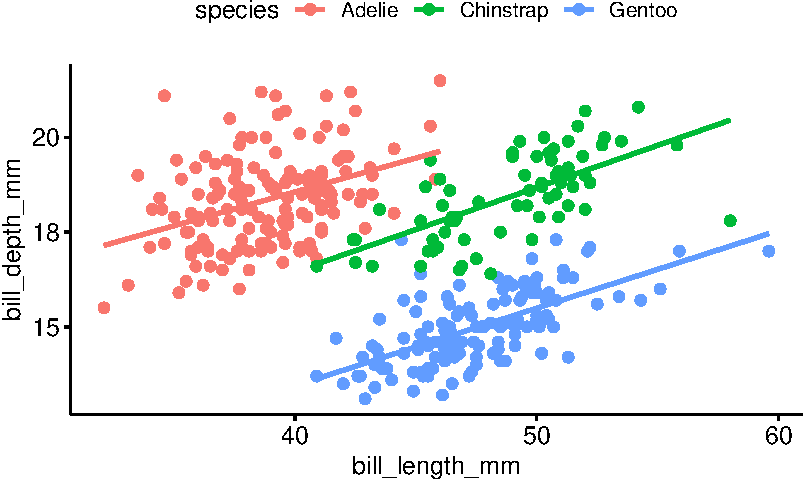
\includegraphics{090-regression2_files/figure-pdf/unnamed-chunk-65-1.pdf}

Oh nein! Was ist hier nur los? Daten lügen nicht, oder doch?

Hier sind die statistischen Details der zweiten Analyse, s.
Tabelle~\ref{tbl-peng-simpson2}. Im zweiten Modell kam \texttt{species}
als zweiter Prädiktor neu ins Modell (zusätlzich zur Schnabellänge).

\begin{Shaded}
\begin{Highlighting}[]
\NormalTok{lm2 }\OtherTok{\textless{}{-}} \FunctionTok{lm}\NormalTok{(bill\_depth\_mm }\SpecialCharTok{\textasciitilde{}}\NormalTok{ bill\_length\_mm }\SpecialCharTok{+}\NormalTok{ species, }\AttributeTok{data =}\NormalTok{ penguins)}
\end{Highlighting}
\end{Shaded}

\begin{longtable}[]{@{}
  >{\raggedright\arraybackslash}p{(\columnwidth - 10\tabcolsep) * \real{0.2817}}
  >{\centering\arraybackslash}p{(\columnwidth - 10\tabcolsep) * \real{0.1831}}
  >{\centering\arraybackslash}p{(\columnwidth - 10\tabcolsep) * \real{0.0845}}
  >{\centering\arraybackslash}p{(\columnwidth - 10\tabcolsep) * \real{0.2254}}
  >{\centering\arraybackslash}p{(\columnwidth - 10\tabcolsep) * \real{0.1127}}
  >{\centering\arraybackslash}p{(\columnwidth - 10\tabcolsep) * \real{0.1127}}@{}}

\caption{\label{tbl-peng-simpson2}Koeffizienten des Modells 2: Positiver
Effekt von bill\_length\_mm}

\tabularnewline

\toprule\noalign{}
\begin{minipage}[b]{\linewidth}\raggedright
Parameter
\end{minipage} & \begin{minipage}[b]{\linewidth}\centering
Coefficient
\end{minipage} & \begin{minipage}[b]{\linewidth}\centering
SE
\end{minipage} & \begin{minipage}[b]{\linewidth}\centering
95\% CI
\end{minipage} & \begin{minipage}[b]{\linewidth}\centering
t(338)
\end{minipage} & \begin{minipage}[b]{\linewidth}\centering
p
\end{minipage} \\
\midrule\noalign{}
\endhead
\bottomrule\noalign{}
\endlastfoot
(Intercept) & 10.59 & 0.68 & (9.25, 11.94) & 15.51 & \textless{} .001 \\
bill length mm & 0.20 & 0.02 & (0.17, 0.23) & 11.43 & \textless{}
.001 \\
species (Chinstrap) & -1.93 & 0.22 & (-2.37, -1.49) & -8.62 &
\textless{} .001 \\
species (Gentoo) & -5.11 & 0.19 & (-5.48, -4.73) & -26.67 & \textless{}
.001 \\

\end{longtable}

\begin{tcolorbox}[enhanced jigsaw, bottomtitle=1mm, title=\textcolor{quarto-callout-caution-color}{\faFire}\hspace{0.5em}{Daten alleine reichen nicht}, toptitle=1mm, arc=.35mm, bottomrule=.15mm, breakable, colbacktitle=quarto-callout-caution-color!10!white, left=2mm, colframe=quarto-callout-caution-color-frame, colback=white, opacityback=0, titlerule=0mm, rightrule=.15mm, opacitybacktitle=0.6, leftrule=.75mm, toprule=.15mm, coltitle=black]

Ohne Hintergrundwissen oder ohne weitere Analysen kann \emph{nicht}
entschieden werden, welche Analyse - Gesamtdaten oder Subgruppen - die
richtige ist. Nicht-exprimentelle Studien können zu grundverschiedenen
Ergebnissen führen, jenachdem ob Prädiktoren dem Modell hinzugefügt oder
weggenommen werden. \(\square\)

\end{tcolorbox}

\subsection{Vorsicht bei der Interpretation von
Regressionskoeffizienten}\label{vorsicht-bei-der-interpretation-von-regressionskoeffizienten}

\begin{tcolorbox}[enhanced jigsaw, bottomtitle=1mm, title=\textcolor{quarto-callout-important-color}{\faExclamation}\hspace{0.5em}{Wichtig}, toptitle=1mm, arc=.35mm, bottomrule=.15mm, breakable, colbacktitle=quarto-callout-important-color!10!white, left=2mm, colframe=quarto-callout-important-color-frame, colback=white, opacityback=0, titlerule=0mm, rightrule=.15mm, opacitybacktitle=0.6, leftrule=.75mm, toprule=.15mm, coltitle=black]

Interpretiere nie Modellkoeffizienten kausal ohne ein
Kausalmodell.\(\square\)

\end{tcolorbox}

Nur wenn man die Ursache-Wirkungs-Beziehungen in einem System kennt,
macht es Sinn, die Modellkoeffizienten kausal zu interpretieren.
Andernfalls lässt man besser die Finger von der Interpretation der
Modellkoeffizienten und begnügt sich mit der Beschreibung der Modellgüte
und mit Vorhersage\footnote{synonym: Prognose}. Wer das nicht glaubt,
der betrachte Abbildung~\ref{fig-confounder}, links.\footnote{\href{https://data-se.netlify.app/2021/12/01/simulation-on-controlling-confounders/}{Quelle}}
Ei Forschi stellt das Modell \texttt{m1:\ y\ \textasciitilde{}\ x} auf
und interpretiert dann \texttt{b1}: ``Ist ja klar, X hat einen starken
positiven Effekt auf Y!''.

In der nächsten Studie nimmt dis Forschi dann eine zweite Variable,
\texttt{group} (z.B. Geschlecht) in das Modell auf:
\texttt{m2:\ y\ \textasciitilde{}\ x\ +\ g}. Oh Schreck! Jetzt ist
\texttt{b1} auf einmal nicht mehr stark positiv, sondern praktisch Null,
und zwar in jeder Gruppe, s. Abbildung~\ref{fig-confounder}, rechts!

Dieses Umschwenken der Regressionskoeffizienten kann \emph{nicht}
passieren, wenn der Effekt ``echt'', also kausal, ist. Handelt es sich
aber um ``nicht echte'', also nicht-kausale Zusammenhänge, um
Scheinzusammenhänge also, so können sich die Modellkoeffizienten
dramatisch verändern (sogar das Vorzeichen kann wechseln\footnote{das
  nennt man dann \emph{Simpsons Paradox}}), wenn man das Modell
verändert, also Variablen hinzufügt oder aus dem Modell entfernt.

Wenn man die kausalen Abhängigkeiten nicht kennt, weiß man also nicht,
ob die Zusammenhänge kausal oder nicht-kausal sind. Man weiß also nicht,
ob die Modellkoeffizienten belastbar, robust, stichhaltig sind oder
nicht.

\begin{figure}

\begin{minipage}{0.50\linewidth}

\centering{

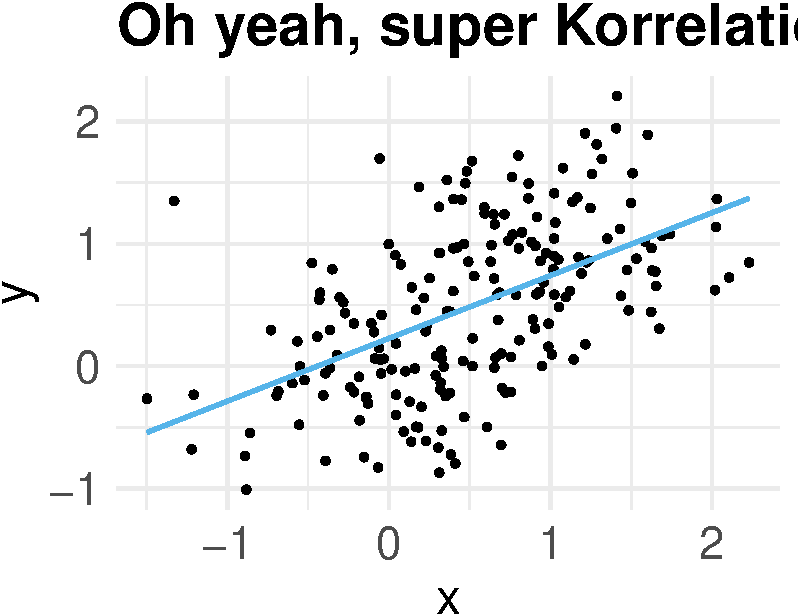
\includegraphics{090-regression2_files/figure-pdf/fig-confounder-1.pdf}

}

\subcaption{\label{fig-confounder-1}Modell:
\texttt{y\ \textasciitilde{}\ x}, starker Zusammenhang; b1 ist stark
positiv}

\end{minipage}%
%
\begin{minipage}{0.50\linewidth}

\centering{

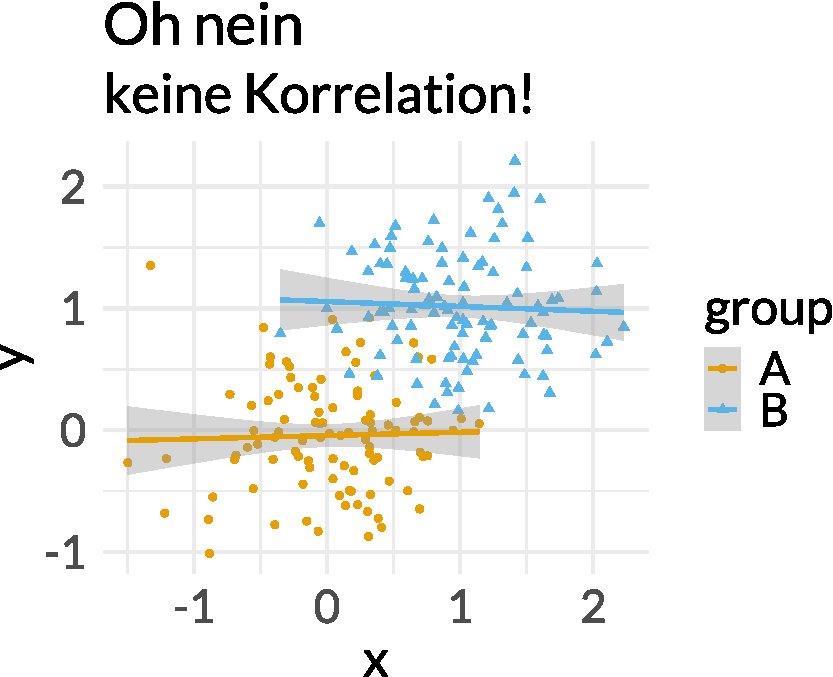
\includegraphics{090-regression2_files/figure-pdf/fig-confounder-2.pdf}

}

\subcaption{\label{fig-confounder-2}Modell:
\texttt{y\ \textasciitilde{}\ x\ +\ g}, in jeder der beiden Gruppen ist
der Zusammenhang praktisch Null, b1 = 0}

\end{minipage}%

\caption{\label{fig-confounder}Fügt man in ein Modell eine Variable
hinzu, können sich die Koeffizienten massiv ändern. In beiden Diagrammen
wurden die gleichen Daten verwendet.}

\end{figure}%

Man könnte höchstens sagen, dass man (wenn man die Kausalstruktur nicht
kennt) die Modellkoeffizienten nur \emph{deskriptiv} interpretiert, z.B.
``Dort wo es viele Störche gibt, gibt es auch viele Babies''.\footnote{Das
  Störche-Babies-Beispiel passt auch zu Abbildung~\ref{fig-confounder}.}
Leider ist unser Gehirn auf kausale Zusammenhänge geprägt: Es fällt uns
schwer, Zusammenhänge nicht kausal zu interpretieren. Daher werden
deskriptive Befunde immer wieder unzulässig kausal interpretiert -- von
Laien und Wissenschaftlern auch.

\section{Fazit}\label{fazit}

In diesem Kapitel haben Sie lineare Modelle gelernt, die über einfache
Modelle der Art \texttt{y\ \textasciitilde{}\ x} hinausgehen. Dazu
gehören multiple Modelle, das sind Modelle mit mehr als einer UV
(Prädiktor) und auch Interaktionsmodelle. Außerdem haben Sie sich mit
einem Datensatz von gesamtgesellschaftlichen Nutzen beschäftigt - sehr
schön. Das Fallbeispiel zum Schluss war vielleicht erhellend insofern,
als dass ein gutes Modell im Train-Sample nicht (notwendig) zu guten
Vorhersagen im Test-Sample führt.

\begin{tcolorbox}[enhanced jigsaw, bottomtitle=1mm, title=\textcolor{quarto-callout-important-color}{\faExclamation}\hspace{0.5em}{Wichtig}, toptitle=1mm, arc=.35mm, bottomrule=.15mm, breakable, colbacktitle=quarto-callout-important-color!10!white, left=2mm, colframe=quarto-callout-important-color-frame, colback=white, opacityback=0, titlerule=0mm, rightrule=.15mm, opacitybacktitle=0.6, leftrule=.75mm, toprule=.15mm, coltitle=black]

Wenn Sie dran bleiben an der Statistik, wird der Erfolg sich einstellen,
s. Abbildung~\ref{fig-dranbleiben}. \(\square\)

\end{tcolorbox}

\begin{figure}

\begin{minipage}{0.50\linewidth}

\centering{


\includegraphics{img/meme-stat1.jpg}

}

\subcaption{\label{fig-gestern}So ging es Ihnen gestern}

\end{minipage}%
%
\begin{minipage}{0.50\linewidth}

\centering{


\includegraphics{img/meme-stat2.jpg}

}

\subcaption{\label{fig-morgen}So wird es Ihnen morgen ergehen, wenn Sie
dran bleiben}

\end{minipage}%

\caption[\label{fig-dranbleiben}Statistik, Sie und Party: Gestern und
(vielleicht) morgen.]{\label{fig-dranbleiben}Statistik, Sie und Party: Gestern und
(vielleicht) morgen.\footnotemark{}}

\end{figure}%
\footnotetext{Quelle: imgflip,
  \url{https://imgflip.com/memegenerator/Distracted-Boyfriend}}

\section{Fallstudien}\label{fallstudien}

Die folgenden Fallstudien zeigen auf recht anspruchsvollem Niveau
(bezogen auf diesen Kurs) beispielhalft zwei ausführlichere
Entwicklungen eines Prognosemodells.

Nutzen Sie diese Fallstudien, um sich intensiver mit der Entwicklung
eines Prognosemodells auseinander zu setzen.

\subsection{New Yorker Flugverspätungen
2023}\label{new-yorker-flugverspuxe4tungen-2023}

\href{https://datenwerk.netlify.app/posts/flights-delay-simplified//}{Vorhersage
von Flugverspätungen}

\subsection{Filmerlöse}\label{filmerluxf6se}

\href{https://data-se.netlify.app/2020/11/13/fallstudie-zur-regressionsanalyse-ggplot2movies/}{Vorhersagen
von Filmerlösen}

\section{Vertiefung}\label{vertiefung}

\href{https://allisonhorst.com/linear-regression-dragons}{Allison Horst}
erklärt die lineare Regression mit Hilfe von Drachen. Sehenswert.

\section{Aufgaben}\label{aufgaben}

Die Webseite
\href{https://datenwerk.netlify.app}{datenwerk.netlify.app}\footnote{\url{https://datenwerk.netlify.app}}
stellt eine Reihe von einschlägigen Übungsaufgaben bereit. Sie können
die Suchfunktion der Webseite nutzen, um die Aufgaben mit den folgenden
Namen zu suchen:

\begin{itemize}
\tightlist
\item
  \href{https://datenwerk.netlify.app/posts/interpret-koeff-lm/interpret-koeff-lm.html}{interpret-koeff-lm}
\item
  \href{https://datenwerk.netlify.app/posts/aussagen-einfache-regr/aussagen-einfache-regr}{Aussagen-einfache-Regr}
\item
  \href{https://datenwerk.netlify.app/posts/interpret-koeff/interpret-koeff.html}{interpret-koeff}
\item
  \href{https://datenwerk.netlify.app/posts/regression1b/regression1b.html}{regression1b}
\item
  \href{https://datenwerk.netlify.app/posts/mtcars-regr01/mtcars-regr01.html}{mtcars-regr01}
\item
  \href{https://datenwerk.netlify.app/posts/regression1a/regression1a.html}{regression1a}
\item
  \href{https://datenwerk.netlify.app/posts/lm1/lm1.html}{lm1}
\item
  \href{https://datenwerk.netlify.app/posts/regression5/regression5}{Regression5}
\item
  \href{https://datenwerk.netlify.app/posts/regression6/regression6}{Regression6}
\item
  \href{https://datenwerk.netlify.app/posts/lm-mario1/lm-mario1.html}{lm-mario1}
\item
  \href{https://datenwerk.netlify.app/posts/lm-mario2/lm-mario2.html}{lm-mario2}
\item
  \href{https://datenwerk.netlify.app/posts/lm-mario3/lm-mario3.html}{lm-mario3}
\item
  \href{https://datenwerk.netlify.app/posts/ausreisser1/ausreisser1.html}{ausreisser1}
\item
  \href{https://datenwerk.netlify.app/posts/mario-compare-models/}{mario-compare-models}
\end{itemize}

\section{Literaturhinweise}\label{literaturhinweise}

Wenn es ein Standardwerk für Regressionsanalyse geben könnte, dann
vielleicht das neueste Buch von Andrew Gelman, ein bekannter Statistiker
(Gelman, Hill, und Vehtari 2021). Sein Buch ist für
Sozialwissenschaftler geschrieben, also nicht für typische Nerds, hat
aber deutlich mehr Anspruch als dieses Kapitel.

\section*{Literatur}\label{literatur}
\addcontentsline{toc}{section}{Literatur}

\phantomsection\label{refs}
\begin{CSLReferences}{1}{0}
\bibitem[\citeproctext]{ref-world_economic_forum_future_2020}
Forum, World Economic. 2020. {„The {Future} of {Jobs Report} 2020``}.
CH-1223 Cologny/Geneva Switzerland: World Economic Forum.
\url{https://www3.weforum.org/docs/WEF_Future_of_Jobs_2020.pdf}.

\bibitem[\citeproctext]{ref-gelman_regression_2021}
Gelman, Andrew, Jennifer Hill, und Aki Vehtari. 2021. \emph{Regression
and Other Stories}. Analytical Methods for Social Research. Cambridge:
Cambridge University Press.

\bibitem[\citeproctext]{ref-okabeito}
Okabe, Masataka, und Kei Ito. 2023. {„Color {Universal Design} ({CUD}) /
{Colorblind Barrier Free}``}. 2023.
\url{https://jfly.uni-koeln.de/color/}.

\end{CSLReferences}




\end{document}
